% -*- latex -*-
%
% The SAND document class is maintained at:
%
%    http://www.cs.sandia.gov/SANDreport
%
% This page also has instructions and documentation on commands.
%
\documentclass[12pt,report]{SANDreport}

\SANDnum{SAND20XX-XXXX}
\SANDprintDate{January 20XX}

\title{VTK-m Users' Guide \\
  \relsize{-2}Version 0.0
}
\author{Kenneth~Moreland \\
  \relsize{-2} Scalable Analysis and Visualization \\[-1ex]
  \relsize{-2} Sandia National Laboratories \\[-1ex]
  \relsize{-2} P.O. Box 5800 MS 1323 \\[-1ex]
  \relsize{-2} Albuquerque, NM 87185-1323 \\[-1ex]
  \relsize{-2} kmorel@sandia.gov
}
\SANDauthor{Kenneth~Moreland}
\date{} % Leave empty


\usepackage{amsfonts}
\usepackage{amssymb}
\usepackage{amsmath}
\usepackage{booktabs}
\usepackage{graphicx}
\usepackage{isomath}
\usepackage{varioref}
\usepackage{fancyvrb}
\usepackage{ifthen}
\usepackage{longtable}
\usepackage{cite}
\usepackage{relsize}
\usepackage{subfig}
\usepackage{xspace}

% This wonderful package allows hyphenation in tt fonts and hyphenation of
% words with underscores in them.
\usepackage[htt]{hyphenat}

% This package defines a tt font that supports boldface (albeit not very
% distinctly). The default package has no boldface for tt fonts.
\usepackage{lmodern}

\usepackage{makeidx}
\makeindex

\usepackage[pdfborder={0 0 0}]{hyperref}
\usepackage{verbatim}

\usepackage{color}
\definecolor{yellow}{rgb}{1,1,0}
\definecolor{black}{rgb}{0,0,0}
\definecolor{ltcyan}{rgb}{.75,1,1}
\definecolor{red}{rgb}{1,0,0}
\definecolor{gray}{rgb}{.6,.6,.6}
\definecolor{darkred}{rgb}{0.5,0,0}
\definecolor{darkgreen}{rgb}{0,0.5,0}

\definecolor{vtkmidentifier}{rgb}{0,0,1}
\definecolor{vtkmnamespace}{rgb}{0.5,0,0}
\definecolor{vtkmmacro}{rgb}{0.5,0,0}
\definecolor{vtkmsignature}{rgb}{0,0.5,0}

\usepackage{listings}
\lstloadlanguages{C,C++}
\lstset{fontadjust=false,basicstyle=\scriptsize\ttfamily}
%% \lstset{numbers=left, numberstyle=\tiny, stepnumber=1, numbersep=2pt}
\lstdefinelanguage{VTKm}{
  morekeywords={struct,class,public,typedef,void,template,return,operator,const,for,int},
  morekeywords={[2]Id,Id2,Id3,IdComponent,Vec,
                   Int8,Int16,Int32,Int64,UInt8,UInt16,UInt32,UInt64,
                   Float32,Float64
                   make_Id3,make_Vec,
                   dot,NUM_COMPONENTS,
                   Extent,Extent3,Pair,
                   ExtentPointDimensions,ExtentCellDimensions,
                   ExtentNumberOfPoints,ExtentNumberOfCells,
                   ExtentPointFlatIndexToTopologyIndex,
                   ExtentCellFlatIndexToTopologyIndex,
                   ExtentPointTopologyIndexToFlatIndex,
                   ExtentCellTopologyIndexToFlatIndex,
                   ExtentFirstPointOnCell,
                   ListTagEmpty,
                   ListTagBase,
                   ListTagJoin,
                   ListForEach,
                   TypeListTagId,TypeListTagId2,TypeListTagId3,
                   TypeListTagIndex,
                   TypeListTagFieldScalar,TypeListTagScalarAll,
                   TypeListTagFieldVec2,
                   TypeListTagFieldVec3,
                   TypeListTagFieldVec4,
                   TypeListTagField,
                   TypeListTagVecCommon,TypeListTagVecAll,
                   TypeListTagAll,TypeListTagCommon,
                   WorkletMapField, WorkletMapCell,
                   WorkletGenerateTopology, WorkletInterpolatedCell,
                   WorkletGenerateKeysValues, WorkletReduceKeysValues,
                   ExecutionObjectBase,
                   TypeTraits,NumericTag,DimensionalityTag,
                   TypeTraitsRealTag,TypeTraitsIntegerTag,
                   TypeTraitsScalarTag,TypeTraitsVectorTag,
                   VecTraits,ComponentType,HasMultipleComponents,
                   VecTraitsTagMultipleComponents,
                   VecTraitsTagSingleComponent,
                   Error, ErrorExecution, ErrorControl,
                   ErrorControlAssert, ErrorControlBadValue,
                   ErrorControlInternal, ErrorControlOutOfMemory,
                   DeviceAdapterTagSerial,
                   DeviceAdapterTagCuda,
                   DeviceAdapterTagOpenMP,
                   DeviceAdapterTagTBB,
                   CellAverage,
                   CellDataToPointDataGenerateKeys,CellDataToPointDataReduceKeys,
                   CellGradient,
                   Cosine,Sine,Magnitude,Square,
                   Elevation,
                   MarchingCubesClassify,MarchingCubesGenerate,
                   PointDataToCellData,
                   SliceClassify,SliceGenerate,
                   Tetrahedralize,
                   ThresholdClassify,ThresholdTopology,
                   ArrayHandle,make_ArrayHandle,
                   ArrayHandleConstant,make_ArrayHandleConstant,
                   ArrayHandleCounting,make_ArrayHandleCounting,
                   ArrayPortalToIterators,
                   ArrayPortalToIteratorBegin,ArrayPortalToIteratorEnd,
                   ArrayContainerControl,
                   ArrayContainerControlTagBasic,
                   ArrayContainerControlTagImplicit,
                   ArrayTransfer,
                   ArrayManagerExecution,
                   ArrayManagerExecutionShareWithControl,
                   DynamicArrayHandle,
                   DynamicPointCoordinates,
                   PointCoordinatesArray,PointCoordinatesUniform,
                   PointCoordinatesBase,
                   PointCoordinatesListTagCommon,
                   DeviceAdapterAlgorithm, DeviceAdapterAlgorithmGeneral,
                   IteratorFromArrayPortal,
                   UniformGrid,UnstructuredGrid,
                   DispatcherMapField, DispatcherMapCell,
                   DispatcherGenerateTopology, DispatcherInterpolatedCell,
                   DispatcherGenerateKeysValues,
                   DispatcherReduceKeysValues,
                   TypeCheck,TypeCheckTagArray,TypeCheckTagExecObject,
                   Transport,
                   TransportTagArrayIn,TransportTagArrayOut,
                   TransportTagExecObject,
                   Fetch,
                   FetchTagArrayDirectIn,FetchTagArrayDirectOut,
                   FetchTagExecObject,
                   AspectTagDefault,
                   Invocation,
                   FunctionInterface,make_FunctionInterface,
                   FunctionInterfaceReturnContainer,
                   DynamicTransform,
                   CellField, CellVertices,
                   InterpolatedCellPoints,
                   CellTraits,NUM_VERTICES,
                   CellTagHexahedron, CellTagLine, CellTagQuadrilateral,
                   CellTagTetrahedron, CellTagTriangle, CellTagVectex,
                   CellTagVoxel, CellTagWedge,
                   CellTraits,
                   CellTopologicalDimensionsTag,
                   GridTagUniform, GridTagUnstructured,
                   NUM_VERTICES, TOPOLOGICAL_DIMENSIONS,
                   ParametricCoordinates, CellDerivative,
                   SortLess, SortGreater,
                   Max, Min,
                   Cbrt, Exp, Exp10, Exp2, ExpM1, Log, Log10, Log1P, Log2,
                   Pow, RCbrt, RSqrt, Sqrt,
                   Matrix, Matrix2x2, Matrix3x3, Matrix4x4,
                   MatrixColumn, MatrixDeterminant, MatrixIdentity,
                   MatrixInverse, MatrixMultiply, MatrixRow,
                   MatrixSetColumn, MatrixSetRow, MatrixTranspose,
                   SolveLinearSystem,
                   NewtonsMethod,
                   Ceil, Epsilon, Floor, FMod, Infinity, IsFinite, IsInf,
                   IsNan, ModF, Nan, NegativeInfinity, Remainder,
                   RemainderQuotient, Round,
                   Abs, CopySign, IsNegative, SignBit,
                   ACos, ACosH, ASin, ASinH, ATan, ATan2, ATanH, Cos, CosH,
                   Pi, Sin, SinH, Tan, TanH,
                   Cross, Magnitude, MagnitudeSquared, Lerp, Normal,
                   Normalize, RMagnitude, TriangleNormal,
                   ParametricCoordinatesToWorldCoordinates,
                   WorldCoordinatesToParametricCoordinates,
                   ParametricCoordinates,
                   TransferToOpenGL
                   },
  morekeywords={[3]VTKM_CONT_EXPORT,VTKM_EXEC_EXPORT,VTKM_EXEC_CONT_EXPORT,
                   VTKM_EXEC_CONSTANT_EXPORT,
                   VTKM_DEVICE_ADAPTER,
                   VTKM_DEVICE_ADAPTER_SERIAL,
                   VTKM_DEVICE_ADAPTER_CUDA,
                   VTKM_DEVICE_ADAPTER_OPENMP,
                   VTKM_DEVICE_ADAPTER_TBB,
                   VTKM_DEVICE_ADAPTER_ERROR,
                   VTKM_DEFAULT_DEVICE_ADAPTER_TAG,
                   VTKM_ARRAY_CONTAINER_CONTROL,
                   VTKM_ARRAY_CONTAINER_CONTROL_BASIC,
                   VTKM_ARRAY_CONTAINER_CONTROL_ERROR,
                   VTKM_DEFAULT_ARRAY_CONTAINER_CONTROL_TAG,
                   VTKM_ASSERT_CONT,
                   VTKM_DEFAULT_TYPE_LIST_TAG,
                   VTKM_DEFAULT_CONTAINER_LIST_TAG,
                   VTKM_DEFAULT_POINT_COORDINATES_LIST_TAG
                   },
  morekeywords={[4]vtkm,exec,cont,worklet,math,arg,internal,detail,
                   cuda,openmp,tbb},
  morekeywords={[5]ControlSignature,ExecutionSignature,InputDomain,
                   FieldIn,FieldOut,
                   FieldPointIn,FieldCellIn,FieldCellOut,
                   TopologyIn,
                   ExecObject,
                   WorkIndex,VisitIndex,
                   IdType,Id2Type,Id3Type,Index,
                   Scalar,ScalarAll,
                   Vec2,Vec3,Vec4,VecAll,
                   FieldCommon,VecCommon,
                   CommonTypes,AllTypes,
                   _1,_2,_3,_4,_5,_6,_7,_8,_9
                   }
}
\lstset{language=VTKm}
\lstset{
  keywordstyle=\bfseries,
  keywordstyle=[2]\color{vtkmidentifier},
  keywordstyle=[3]\color{vtkmmacro},
  keywordstyle=[4]\color{vtkmnamespace},
  keywordstyle=[5]\color{vtkmsignature}
}

\renewcommand{\lstlistlistingname}{List of Examples}
\renewcommand{\lstlistingname}{Example}

\newcommand*{\textcode}[1]{\texttt{#1}}
\newcommand*{\textnamespace}[1]{\textcode{\color{vtkmnamespace}{#1}}}
\newcommand*{\textmacro}[1]{\textcode{\color{vtkmmacro}{#1}}}
\newcommand*{\textidentifier}[1]{\textcode{\color{vtkmidentifier}{#1}}}
\newcommand*{\textsignature}[1]{\textcode{\color{vtkmsignature}{#1}}}

\newcommand*{\vtkmmacro}[1]{\textmacro{#1}\index{#1}}

\newcommand{\vtkmcontexport}{\vtkmmacro{VTKM\_CONT\_EXPORT}\index{export!control}\index{function~export}\index{method~export}\xspace}
\newcommand{\vtkmexecexport}{\vtkmmacro{VTKM\_EXEC\_EXPORT}\index{export!execution}\index{function~export}\index{method~export}\xspace}
\newcommand{\vtkmexeccontexport}{\vtkmmacro{VTKM\_EXEC\_CONT\_EXPORT}\index{export!control}\index{export!execution}\index{function~export}\index{method~export}\xspace}

\newcommand{\controlsignature}{\textsignature{ControlSignature}\index{control~signature}\index{signature!control}\xspace}
\newcommand{\executionsignature}{\textsignature{ExecutionSignature}\index{execution~signature}\index{signature!execution}\xspace}
\newcommand{\inputdomain}{\textsignature{InputDomain}\index{input~domain}\xspace}

\newcommand*{\sigtag}[1]{\textsignature{#1}\index{#1}\index{signature tags!#1}}
\newcommand*{\sigtagnum}[1]{\sigtag{\_#1}}
\newcommand*{\sigtagmod}[2]{\sigtag{#1}\textcode{<}\sigtag{#2}\textcode{>}}
\newcommand*{\sigtagmodnum}[2]{\sigtag{#1}\textcode{<}\sigtagnum{#2}\textcode{>}}

\newcommand*{\writenamespaceone}[1]{%
  \textnamespace{#1}}
\newcommand*{\writenamespacetwo}[2]{%
  \writenamespaceone{#1}\textcode{:\colonhyp}\textnamespace{#2}}
\newcommand*{\writenamespacethree}[3]{%
  \writenamespacetwo{#1}{#2}\textcode{:\colonhyp}\textnamespace{#3}}
\newcommand*{\writenamespacefour}[4]{%
  \writenamespacethree{#1}{#2}{#3}\textcode{:\colonhyp}\textnamespace{#4}}

\newcommand*{\indexnamespaceone}[1]{%
  \index{#1 namespace}\index{namespace!#1}}
\newcommand*{\indexnamespacetwo}[2]{%
  \index{#2 namespace}\index{#1::#2}\index{namespace!#1::#2}}
\newcommand*{\indexnamespacethree}[3]{%
  \index{#3 namespace}\index{#1::#2::#3}\index{namespace!#1::#2::#3}}
\newcommand*{\indexnamespacefour}[4]{%
  \index{#4 namespace}\index{#1::#2::#3::#4}\index{namespace!#1::#2::#3::#4}}

\newcommand*{\writeindexidentifierone}[2]{%
  \writenamespaceone{#1}\textcode{:\colonhyp}\textidentifier{#2}%
  \index{#2}}
\newcommand*{\writeindexidentifiertwo}[3]{%
  \writenamespacetwo{#1}{#2}\textcode{:\colonhyp}\textidentifier{#3}%
  \index{#3}}
\newcommand*{\writeindexidentifierthree}[4]{%
  \writenamespacethree{#1}{#2}{#3}\textcode{:\colonhyp}\textidentifier{#4}%
  \index{#4}}
\newcommand*{\writeindexidentifierfour}[5]{%
  \writenamespacefour{#1}{#2}{#3}{#4}\textcode{:\colonhyp}\textidentifier{#5}%
  \index{#5}}

\newcommand*{\vtkm}[1]{%
  \ifthenelse{\equal{#1}{}}%
             {\writenamespaceone{vtkm}\indexnamespaceone{vtkm}}%
             {\writeindexidentifierone{vtkm}{#1}}}
\newcommand*{\vtkminternal}[1]{%
  \ifthenelse{\equal{#1}{}}%
             {\writenamespacetwo{vtkm}{internal}\indexnamespacetwo{vtkm}{internal}}%
             {\writeindexidentifiertwo{vtkm}{internal}{#1}}}
\newcommand*{\vtkmcont}[1]{%
  \ifthenelse{\equal{#1}{}}%
             {\writenamespacetwo{vtkm}{cont}\indexnamespacetwo{vtkm}{cont}}%
             {\writeindexidentifiertwo{vtkm}{cont}{#1}}}
\newcommand*{\vtkmcontinternal}[1]{%
  \ifthenelse{\equal{#1}{}}%
             {\writenamespacethree{vtkm}{cont}{internal}\indexnamespacethree{vtkm}{cont}{internal}}%
             {\writeindexidentifierthree{vtkm}{cont}{internal}{#1}}}
\newcommand*{\vtkmcontarg}[1]{%
  \ifthenelse{\equal{#1}{}}%
             {\writenamespacethree{vtkm}{cont}{arg}\indexnamespacethree{vtkm}{cont}{arg}}%
             {\writeindexidentifierthree{vtkm}{cont}{arg}{#1}}}
\newcommand*{\vtkmexec}[1]{%
  \ifthenelse{\equal{#1}{}}%
             {\writenamespacetwo{vtkm}{exec}\indexnamespacetwo{vtkm}{exec}}%
             {\writeindexidentifiertwo{vtkm}{exec}{#1}}}
\newcommand*{\vtkmexecarg}[1]{%
  \ifthenelse{\equal{#1}{}}%
             {\writenamespacethree{vtkm}{exec}{arg}\indexnamespacethree{vtkm}{exec}{arg}}%
             {\writeindexidentifierthree{vtkm}{exec}{arg}{#1}}}
\newcommand*{\vtkmexecinternal}[1]{%
  \ifthenelse{\equal{#1}{}}%
             {\writenamespacethree{vtkm}{exec}{internal}\indexnamespacethree{vtkm}{exec}{internal}}%
             {\writeindexidentifierthree{vtkm}{exec}{internal}{#1}}}
\newcommand*{\vtkmworklet}[1]{%
  \ifthenelse{\equal{#1}{}}%
             {\writenamespacetwo{vtkm}{worklet}\indexnamespacetwo{vtkm}{worklet}}%
             {\writeindexidentifiertwo{vtkm}{worklet}{#1}}}
\newcommand*{\vtkmmath}[1]{%
  \ifthenelse{\equal{#1}{}}%
             {\writenamespacetwo{vtkm}{math}\indexnamespacetwo{vtkm}{math}}%
             {\writeindexidentifiertwo{vtkm}{math}{#1}}}

\newcommand*{\vtkmcuda}[1]{%
  \ifthenelse{\equal{#1}{}}%
             {\writenamespacetwo{vtkm}{cuda}\indexnamespacetwo{vtkm}{cuda}}%
             {\writeindexidentifiertwo{vtkm}{cuda}{#1}}}
\newcommand*{\vtkmcudacont}[1]{%
  \ifthenelse{\equal{#1}{}}%
             {\writenamespacethree{vtkm}{cuda}{cont}\indexnamespacethree{vtkm}{cuda}{cont}}%
             {\writeindexidentifierthree{vtkm}{cuda}{cont}{#1}}}
\newcommand*{\vtkmopenmp}[1]{%
  \ifthenelse{\equal{#1}{}}%
             {\writenamespacetwo{vtkm}{openmp}\indexnamespacetwo{vtkm}{openmp}}%
             {\writeindexidentifiertwo{vtkm}{openmp}{#1}}}
\newcommand*{\vtkmopenmpcont}[1]{%
  \ifthenelse{\equal{#1}{}}%
             {\writenamespacethree{vtkm}{openmp}{cont}\indexnamespacethree{vtkm}{openmp}{cont}}%
             {\writeindexidentifierthree{vtkm}{openmp}{cont}{#1}}}
\newcommand*{\vtkmtbb}[1]{%
  \ifthenelse{\equal{#1}{}}%
             {\writenamespacetwo{vtkm}{tbb}\indexnamespacetwo{vtkm}{tbb}}%
             {\writeindexidentifiertwo{vtkm}{tbb}{#1}}}
\newcommand*{\vtkmtbbcont}[1]{%
  \ifthenelse{\equal{#1}{}}%
             {\writenamespacethree{vtkm}{tbb}{cont}\indexnamespacethree{vtkm}{tbb}{cont}}%
             {\writeindexidentifierthree{vtkm}{tbb}{cont}{#1}}}

\newcommand*{\vtkmopengl}[1]{%
  \ifthenelse{\equal{#1}{}}%
             {\writenamespacetwo{vtkm}{opengl}\indexnamespacetwo{vtkm}{opengl}}%
             {\writeindexidentifiertwo{vtkm}{opengl}{#1}}}

\newcommand*{\tparams}[1]{\textcode{<#1>}}

\newcommand*{\textfilename}[1]{\textsf{#1}}
\newcommand*{\vtkmheader}[2]{%
  \textfilename{#1\fshyp{}#2}\index{#1\fshyp#2}\index{#2}}

\newcommand*{\cmakevar}[1]{%
  \textsf{#1}%
  \index{#1}%
  \index{CMake configuration!#1}}

\lstnewenvironment{vtkmexample}[2][-*-]{
  \lstset{caption={#2}}
  \ifthenelse{\equal{#1}{-*-}}{}{\lstset{label=#1}}
}{
}

\newcommand*{\vtkmlisting}[3][]{
  \lstinputlisting[language=VTKm, label=#1, caption={#2}]{examples/listing_#3}
}

% Cite commands I use to abstract away the different ways to reference an
% entry in the bibliography (superscripts, numbers, dates, or author
% abbreviations).  \scite is a short cite that is used immediately after
% when the authors are mentioned.  \lcite is a full citation that is used
% anywhere.  Both should be used right next to the text being cited without
% any spacing.
\newcommand*{\lcite}[1]{~\cite{#1}}
\newcommand*{\scite}[1]{~\cite{#1}}

\newcommand{\etal}{et al.}

\newcommand*{\keyterm}[1]{\emph{#1}}

\newcommand{\fix}[1]{{\color{red}\textsc{[#1]}}}
%\newcommand{\fix}[1]{}

% Avoid putting figures on their own page.
\renewcommand{\textfraction}{0.05}
\renewcommand{\topfraction}{0.95}
\renewcommand{\bottomfraction}{0.95}

% Make sure this is big enough so that only big figures end up on their own
% page but small enough so that if a figure does have to be on its own
% page, it won't push everything to the bottom because it's not big enough
% to have its own page.
\renewcommand{\floatpagefraction}{.75}

% Environments for tightly packed lists.
\newenvironment{enumeratetight}{
  \begin{enumerate}
    \setlength{\topsep}{0pt}
    \setlength{\itemsep}{0pt}
    \setlength{\parskip}{0pt}
    \setlength{\parsep}{0pt}
    \setlength{\partopsep}{0pt}
}{
  \end{enumerate}
}

\newenvironment{itemizetight}{
  \begin{itemize}
    \setlength{\topsep}{0pt}
    \setlength{\itemsep}{0pt}
    \setlength{\parskip}{0pt}
    \setlength{\parsep}{0pt}
    \setlength{\partopsep}{0pt}
}{
  \end{itemize}
}

\newenvironment{descriptiontight}{
  \begin{description}
    \setlength{\topsep}{0pt}
    \setlength{\itemsep}{0pt}
    \setlength{\parskip}{0pt}
    \setlength{\parsep}{0pt}
    \setlength{\partopsep}{0pt}
}{
  \end{description}
}

\begin{document}

\sloppy

\maketitle

\begin{abstract}
  \fix{Write this.}
\end{abstract}

\clearpage

\chapter*{Acknowledgement}

\fix{Write this. Can steal from Dax document.}


\cleardoublepage % TOC should start on an odd page
\tableofcontents
\listoffigures
%\listoftables
\lstlistoflistings

\clearpage

\SANDmain

% -*- latex -*-

\chapter{Introduction}
\label{chap:Introduction}

High-performance computing relies on ever finer threading. Advances in
processor technology include ever greater numbers of cores, hyperthreading,
accelerators with integrated blocks of cores, and special vectorized
instructions, all of which require more software parallelism to achieve
peak performance. Traditional visualization solutions cannot support this
extreme level of concurrency. Extreme scale systems require a new
programming model and a fundamental change in how we design algorithms. To
address these issues we created VTK-m: the visualization toolkit for
multi-/many-core architectures.

VTK-m supports a number of algorithms and the ability to design further
algorithms through a top-down design with an emphasis on extreme
parallelism. VTK-m also provides support for finding and building links
across topologies, making it possible to perform operations that determine
manifold surfaces, interpolate generated values, and find adjacencies.
Although Dax provides a simplified high-level interface for programming,
its template-based code removes the overhead of abstraction.

\begin{figure}[htb]
  \centering
  \begin{tabular}{ccc}
    CUDA SDK & PISTON & VTK-m \\
    {\small 431 LOC} & {\small 369 LOC} & {\small 265 LOC} \\
    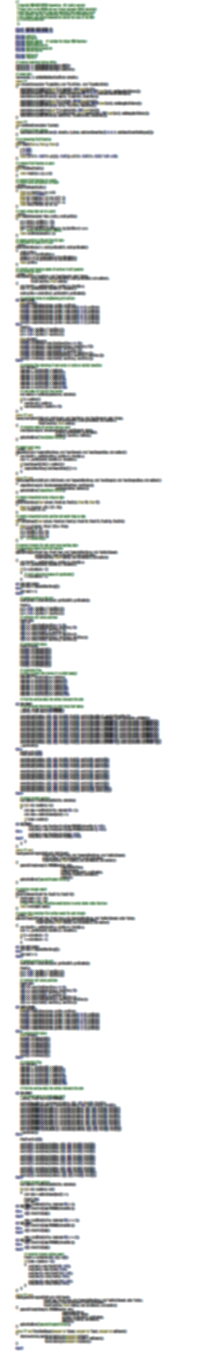
\includegraphics[width=.75in]{images/MCCompareCuda} &
    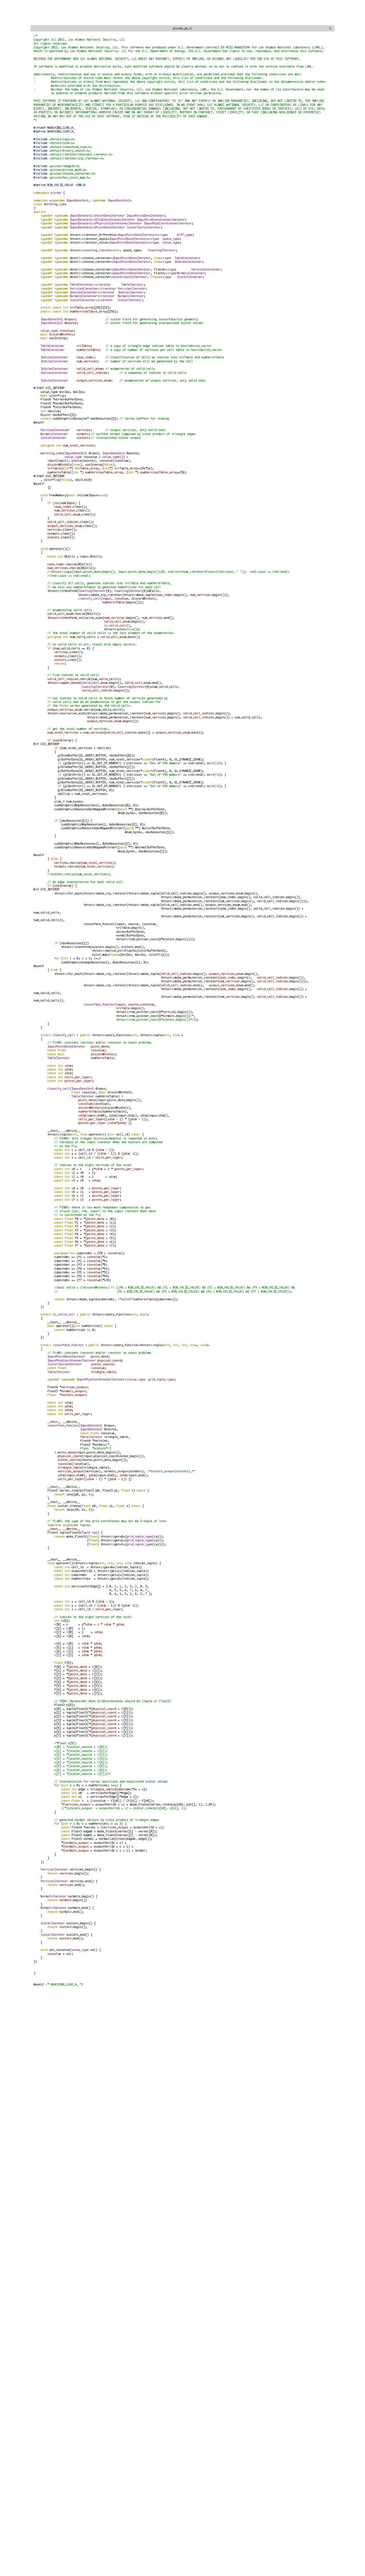
\includegraphics[width=.75in]{images/MCComparePiston} &
    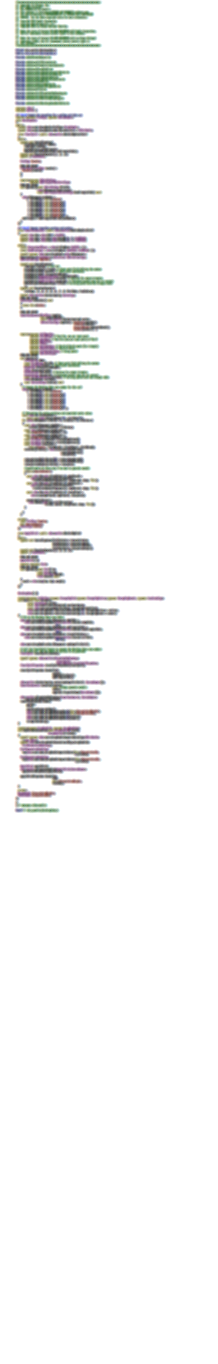
\includegraphics[width=.75in]{images/MCCompareVTKm}
  \end{tabular}
  \caption[Comparison of Marching Cubes implementations.]{Comparison of the
    Marching Cubes algorithm in VTK-m and two other implementations.
    Implementations in VTK-m are simpler, shorter, more general, and easier
    to maintain. (Lines of code (LOC) measurements come from cloc.}
  \label{fig:MCCompare}
\end{figure}

VTK-m simplifies the development of parallel scientific visualization
algorithms by providing a framework of supporting functionality that allows
developers to focus on visualization operations. Consider the listings in
Figure~\ref{fig:MCCompare} that compares the size of the implementations
for the Marching Cubes algorithm in VTK-m with the equivalent algorithms
implemented in the CUDA software development kit reference implementation
and the PISTON visualization library. Because VTK-m internally manages the
parallel distribution of work and data, the VTK-m implementation is shorter
and easier to maintain. Additionally, VTK-m provides data abstractions not
provided by the other libraries that make code written in VTK-m more
versatile.

\begin{didyouknow}
  VTK-m is written in C++ and makes extensive use of templates. The toolkit
  is implemented as a header library, meaning that all the code is
  implemented in header files (with extension \textfilename{.h}) and
  completely included in any code that uses it. This allows the compiler to
  inline and specialize code for better performance.
\end{didyouknow}

\section{How to Use This Guide}

This user's guide is organized into three parts to help guide novice to
advanced users and to provide a convenient reference.
Part~\ref{part:GettingStarted}, Getting Started, provides everything needed
to get up and running with VTK-m. In this part we learn the basics of
reading and writing data files, using filters to process data, and perform
basic rendering to view the results.

Part~\ref{part:Developing}, Developing with VTK-m, dives deeper into the
VTK-m library and provides all the information needed to customize VTK-m's
data structures and support multiple devices. Part~\ref{part:Developing}
also documents how to use VTK-m's framework to develop new or custom
visualization algorithms.

Part~\ref{part:Advanced}, Advanced Customization, exposes the inner
workings of VTK-m and allows you to design new algorithmic structures not
already available. \fix{This might be removed in the first version of the
  book.}

\section{Conventions Used in This Guide}

When documenting the VTK-m API, the following conventions are used.
\begin{itemize}
\item Filenames are printed in a \textfilename{sans serif font}.
\item C++ code is printed in a \textcode{monospace font}.
\item Macros and namespaces from VTK-m are printed in \textnamespace{red}.
\item Identifiers from VTK-m are printed in \textidentifier{blue}.
\item Signatures, described in Chapter~\ref{chap:Worklets}, and the
  tags used in them are printed in \textsignature{green}.
\end{itemize}

This guide provides actual code samples throughout its discussions to
demonstrate their use. These examples are all valid code that can be
compiled and used although it is often the case that code snippets are
provided. In such cases, the code must be placed in a larger context.

\begin{didyouknow}
  In this guide we periodically use these \textbf{Did you know?} boxes to
  provide additional information related to the topic at hand.
\end{didyouknow}

\begin{commonerrors}
  \textbf{Common Errors} blocks are used to highlight some of the common
  problems or complications you might encounter when dealing with the topic
  of discussion.
\end{commonerrors}


% -*- latex -*-

\chapter{Basic Provisions}
\label{chap:BasicProvisions}

This section describes the core facilities provided by VTK-m. These include
macros, types, and classes that define the environment in which code is
run, the core types of data stored, and template introspection. We also
start with a description of package structure used by VTK-m.


\section{General Approach}
\label{sec:GeneralApproach}

VTK-m is designed to provide a \keyterm{pervasive parallelism}
\index{pervasive parallelism} throughout all its visualization algorithms,
meaning that the algorithm is designed to operate with independent
concurrency at the finest possible level throughout. VTK-m provides this
pervasive parallelism by providing a programming construct called a
\keyterm{worklet}, \index{worklet} which operates on a very fine
granularity of data. The worklets are designed as serial components, and
VTK-m handles whatever layers of concurrency are necessary, thereby
removing the onus from the visualization algorithm developer. Worklet
operation is then wrapped into \keyterm{filters}, \index{filter} which
provide a simplified interface to end users.

A worklet is essentially a small functor \index{functor} or kernel
\index{kernel} designed to operate on a small element of data. (The name
``worklet'' means a small amount of work. We mean small in this sense to be
the amount of data, not necessarily the amount of instructions performed.)
The worklet is constrained to contain a serial and stateless function.
These constraints form three critical purposes. First, the constraints on
the worklets allow VTK-m to schedule worklet invocations on a great many
independent concurrent threads and thereby making the algorithm pervasively
parallel. Second, the constraints allow VTK-m to provide thread safety. By
controlling the memory access the toolkit can insure that no worklet will
have any memory collisions, false sharing, or other parallel programming
pitfalls. Third, the constraints encourage good programming practices. The
worklet model provides a natural approach to visualization algorithm design
that also has good general performance characteristics.

VTK-m allows developers to design algorithms that are run on massive
amounts of threads. However, VTK-m also allows developers to interface to
applications, define data, and invoke algorithms that they have written or
are provided otherwise. These two modes represent significantly different
operations on the data. The operating code of an algorithm in a worklet is
constrained to access only a small portion of data that is provided by the
framework. Conversely, code that is building the data structures needs to
manage the data in its entirety, but has little reason to perform
computations on any particular element.

Consequently, VTK-m is divided into two \keyterm{environments}
\index{environment} that handle each of these use cases. Each environment
has its own API, and direct interaction between the environments is
disallowed. The environments are as follows.

\begin{description}
\item[Execution Environment] \index{execution environment}
  \index{environment!execution} This is the environment in which the
  computational portion of algorithms are executed. The API for this
  environment provides work for one element with convenient access to
  information such as connectivity and neighborhood as needed by typical
  visualization algorithms. Code for the execution environment is designed
  to always execute on a very large number of threads.
\item[Control Environment] \index{control environment}
  \index{environment!control} This is the environment that is used to
  interface with applications, interface with I/O devices, and schedule
  parallel execution of the algorithms. The associated API is designed for
  users that want to use VTK-m to analyze their data using provided or
  supplied filters. Code for the control environment is designed to run on
  a single thread (or one single thread per process in an MPI job).
\end{description}

These dual programming environments are partially a convenience to isolate
the application from the execution of the worklets and are partially a
necessity to support GPU languages with host and device environments. The
control and execution environments are logically equivalent to the host and
device environments, respectively, in CUDA and other associated GPU
languages.

\begin{figure}[htb]
  \centering
  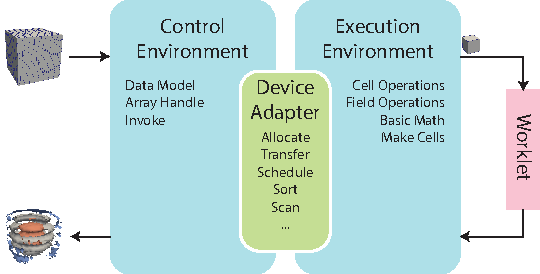
\includegraphics[width=4in]{images/VTKmEnvironments}
  \caption{Diagram of the VTK-m framework.}
  \label{fig:VTKmDiagram}
\end{figure}

Figure~\ref{fig:VTKmDiagram} displays the relationship between the control
and execution environment. The typical workflow when using VTK-m is that
first the control thread establishes a data set in the control environment
and then invokes a parallel operation on the data using a filter. From
there the data is logically divided into its constituent elements, which
are sent to independent invocations of a worklet. The worklet
invocations, being independent, are run on as many concurrent threads as
are supported by the device. On completion the results of the worklet
invocations are collected to a single data structure and a handle is
returned back to the control environment.

\begin{didyouknow}
  Are you only planning to use filters in VTK-m that already exist? If so,
  then everything you work with will be in the control environment. The
  execution environment is only used when implementing algorithms for
  filters.
\end{didyouknow}


\section{Package Structure}
\label{sec:PackageStructure}

\index{packages|(}

VTK-m is organized in a hierarchy of nested packages. VTK-m places
definitions in \keyterm{namespaces} \index{namespace} that correspond to
the package (with the exception that one package may specialize a template
defined in a different namespace).

The base package is named \vtkm{}. All classes within VTK-m are placed
either directly in the \vtkm{} package or in a package beneath it. This
helps prevent name collisions between VTK-m and any other library.

As described in Section~\ref{sec:GeneralApproach}, the VTK-m API is divided
into two distinct environments: \index{environment} the control environment
\index{control environment} \index{environment!control} and the execution
environment. \index{execution environment} \index{environment!execution}
The API for these two environments are located in the \vtkmcont{} and
\vtkmexec{} packages, respectively. Items located in the base \vtkm{}
namespace are available in both environments.

Although it is conventional to spell out names in identifiers (see the
coding conventions in Chapter~\ref{chap:CodingConventions}), there is an
exception to abbreviate control and execution to \textnamespace{cont}
and \textnamespace{exec}, respectively. This is because it is also part of
the coding convention to declare the entire namespace when using an
identifier that is part of the corresponding package. The shorter names
make the identifiers easier to read, faster to type, and more feasible to
pack lines in 80 column displays. These abbreviations are also used instead
of more common abbreviations (e.g. ctrl for control) because, as part of
actual English words, they are easier to type.

Further functionality in VTK-m is built on top of the base \vtkm{},
\vtkmcont{}, and \vtkmexec{} packages. Support classes for building
worklets, described in Chapter~\ref{chap:Worklets}, are contained in the
\vtkmworklet{} package. Other facilities in VTK-m are provided in their own
packages such as \vtkmio{}, \vtkmfilter{}, and \vtkmrendering{}. These
packages are described in Part~\ref{part:GettingStarted}.

VTK-m contains code that uses specialized compiler features, such as those
with CUDA, or libraries, such as Intel Threading Building Blocks, that will
not be available on all machines. Code for these features are encapsulated
in their own packages under the \vtkmcont{} namespace: \vtkmcontcuda{} and
\vtkmconttbb{}.

VTK-m contains OpenGL interoperability \index{OpenGL}
\index{interoperability} that allows data generated with VTK-m to be
efficiently transferred to OpenGL objects. This feature is encapsulated in
the \vtkmopengl{} package.

Figure~\ref{fig:Packages} provides a diagram of the VTK-m package hierarchy.

\begin{figure}[htb]
  \centering
  %% \begin{itemize}
  %% \item \vtkm{}
  %% \item \vtkmexec{}
  %% \item \vtkmcont{}
  %% \item \vtkmcontcuda{}
  %% \item \vtkmconttbb{}
  %% \item \vtkmio{}
  %% \item \vtkmioreader{}
  %% \item \vtkmiowriter{}
  %% \item \vtkmfilter{}
  %% \item \vtkmrendering{}
  %% \item \vtkmopengl{}
  %% \item \vtkmworklet{}
  %% %% \item \textnamespace{vtkm}
  %% %%   \begin{itemize}
  %% %%   \item \textnamespace{cont}
  %% %%   \item \textnamespace{exec}
  %% %%   \item \textnamespace{worklet}
  %% %%   \item \textnamespace{math}
  %% %%   \item \textnamespace{cuda}
  %% %%     \begin{itemize}
  %% %%     \item \textnamespace{cont}
  %% %%     \end{itemize}
  %% %%   \item \textnamespace{openmp}
  %% %%     \begin{itemize}
  %% %%     \item \textnamespace{cont}
  %% %%     \end{itemize}
  %% %%   \item \textnamespace{tbb}
  %% %%     \begin{itemize}
  %% %%     \item \textnamespace{cont}
  %% %%     \end{itemize}
  %% %%   \item \textnamespace{opengl}
  %% %%   \end{itemize}
  %% \end{itemize}
  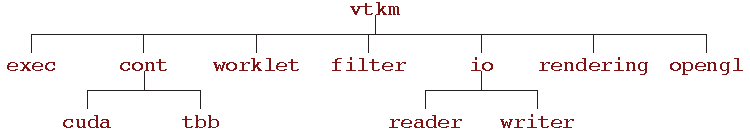
\includegraphics{images/PackageHierarchy}
  \caption{VTK-m package hierarchy.}
  \label{fig:Packages}
\end{figure}

By convention all classes will be defined in a file with the same name as
the class name (with a \textfilename{.h} extension) located in a directory
corresponding to the package name. For example, the \vtkmcont{ArrayHandle}
class is found in the \vtkmheader{vtkm/cont}{ArrayHandle.h} header. There
are, however, exceptions to this rule. Some smaller classes and types are
grouped together for convenience. These exceptions will be noted as
necessary.

Within each namespace there may also
be \textnamespace{internal}\indexnamespaceone{internal}
and \textnamespace{detail}\indexnamespaceone{detail}
sub-namespaces. The \textnamespace{internal} namespaces contain features
that are used internally and may change without
notice. The \textnamespace{detail} namespaces contain features that are
used by a particular class but must be declared outside of that
class. Users should generally ignore classes in these namespaces.

\index{packages|)}


\section{Function and Method Environment Modifiers}
\label{sec:FunctionAndMethodEnvironmentModifiers}

Any function or method defined by VTK-m must come with a modifier that determines in which environments the function may be run.
These modifiers are C macros that VTK-m uses to instruct the compiler for which architectures to compile each method.
Most user code outside of VTK-m need not use these macros with the important exception of any classes passed to VTK-m.
This occurs when defining new worklets, array storage, and device adapters.

VTK-m provides three modifier macros, \vtkmcontmodifier, \vtkmexecmodifier, and
\vtkmexeccontmodifier, which are used to declare functions and methods that
can run in the control environment, execution environment, and both
environments, respectively. These macros get defined by including just
about any VTK-m header file, but including \vtkmheader{vtkm}{Types.h} will
ensure they are defined. 

The modifier macro is placed after the template declaration, if there is one,
and before the return type for the function. Here is a simple example of a
function that will square a value. Since most types you would use this
function on have operators in both the control and execution environments,
the function is declared for both places.

\vtkmlisting{Usage of an environment modifier macro on a function.}{EnvironmentModifierMacro.cxx}

The primary function of the modifier macros is to inject compiler-specific
keywords that specify what architecture to compile code for. For example,
when compiling with CUDA\index{CUDA}, the control modifiers have
\textcode{\_\_host\_\_}\index{\_\_host\_\_} in them and execution modifiers
have \textcode{\_\_device\_\_}\index{\_\_device\_\_} in them.

There is one additional modifier macro that is not used for functions but
rather used when declaring a constant data object that is used in the
execution environment. This macro is named
\vtkmmacro{VTKM\_EXEC\_CONSTANT}\index{modifier!constant}\index{constant modifier}
and is used to declare a constant lookup table used when executing a
worklet. Its primary reason for existing is to add a
\textcode{\_\_constant\_\_} keyword when compiling with CUDA. This modifier
currently has no effect on any other compiler.

Finally, it is sometimes the case that a function declared as
\vtkmexeccontmodifier has to call a method declared as \vtkmexecmodifier or
\vtkmcontmodifier. Generally functions should not call other functions with
incompatible control/execution modifiers, but sometimes a generic
\vtkmexeccontmodifier function calls another function determined by the
template parameters, and the valid environments of this subfunction may be
inconsistent. For cases like this, you can use the
\vtkmmacro{VTKM\_SUPPRESS\_EXEC\_WARNINGS} to tell the compiler to ignore the
inconsistency when resolving the template. When applied to a templated
function or method, \vtkmmacro{VTKM\_SUPPRESS\_EXEC\_WARNINGS} is placed
before the \textcode{template} keyword. When applied to a non-templated
method in a templated class, \vtkmmacro{VTKM\_SUPPRESS\_EXEC\_WARNINGS} is
placed before the environment modifier macro.

\vtkmlisting{Suppressing warnings about functions from mixed environments.}{SuppressExecWarnings.cxx}


\section{Core Data Types}
\label{sec:CoreDataTypes}

Except in rare circumstances where precision is not a concern, VTK-m does
not directly use the core C types like \textcode{int}, \textcode{float},
and \textcode{double}. Instead, VTK-m provides its own core types, which
are declared in \vtkmheader{vtkm}{Types.h}.

\subsection{Single Number Types}

To ensure portability across different compilers and architectures, VTK-m
provides \textcode{typedef}s for the following basic types with explicit
precision: \vtkm{Float32}, \vtkm{Float64}, \vtkm{Int8}, \vtkm{Int16},
\vtkm{Int32}, \vtkm{Int64}, \vtkm{UInt8}, \vtkm{UInt16}, \vtkm{UInt32}, and
\vtkm{UInt64}. Under most circumstances when using VTK-m (and performing
visualization in general) the type of data is determined by the source of the
data or resolved through templates. In the case where a specific type of
data is required, these VTK-m--defined types should be preferred over basic
C types like \textcode{int} or \textcode{float}.

Many of the structures in VTK-m require indices to identify elements like
points and cells. All indices for arrays and other lists use the type
\vtkm{Id}. By default this type is a 32-bit wide integer but can be easily
changed by compile options. The CMake configuration option
\cmakevar{VTKM\_USE\_64BIT\_IDS} can be used to change \vtkm{Id} to be 64
bits wide. This configuration can be overridden by defining the C macro
\vtkmmacro{VTKM\_USE\_64BIT\_IDS} or \vtkmmacro{VTKM\_NO\_64BIT\_IDS} to
force \vtkm{Id} to be either 64 or 32 bits. These macros must be defined
before any VTK-m header files are included to take effect.

There is also a secondary index type named \vtkm{IdComponent} that is used
to index components of short vectors (discussed in
Section~\ref{sec:VectorTypes}). This type is an integer that might be a
shorter width than \vtkm{Id}.

There is also the rare circumstance in which an algorithm in VTK-m computes
data values for which there is no indication what the precision should
be. For these circumstances, the type \vtkm{FloatDefault} is provided. By
default this type is a 32-bit wide floating point number but can be easily
changed by compile options. The CMake configuration option
\cmakevar{VTKM\_USE\_DOUBLE\_PRECISION} can be used to change
\vtkm{FloatDefault} to be 64 bits wide. This configuration can be
overridden by defining the C macro \vtkmmacro{VTKM\_USE\_DOUBLE\_PRECISION}
or \vtkmmacro{VTKM\_NO\_DOUBLE\_PRECISION} to force \vtkm{FloatDefault} to
be either 64 or 32 bits. These macros must be defined before any VTK-m
header files are included to take
effect.

For convenience, you can include either
\vtkmheader{vtkm/internal}{ConfigureFor32.h} or
\vtkmheader{vtkm/internal}{ConfigureFor64.h} to force both \vtkm{Id} and
\vtkm{FloatDefault} to be 32 or 64 bits.

\subsection{Vector Types}
\label{sec:VectorTypes}

Visualization algorithms also often require operations on short vectors.
Arrays indexed in up to three dimensions are common. Data are often defined
in 2-space and 3-space, and transformations are typically done in
homogeneous coordinates of length 4. To simplify these types of operations,
VTK-m provides the \vtkm{Vec}\tparams{T,Size} templated type, which is
essentially a fixed length array of a given type.

The default constructor of \vtkm{Vec} objects leaves the values
uninitialized. All vectors have a constructor with one argument that is
used to initialize all components. All \vtkm{Vec} objects with a size of 4
or less is specialized to also have a constructor that allows you to set
the individual components. Likewise, there is a \vtkm{make\_Vec} function
that builds initialized vector types of up to 4 components. Once created,
you can use the bracket operator to get and set component values with the
same syntax as an array.

\vtkmlisting{Creating vector types.}{CreatingVectorTypes.cxx}

The types \vtkm{Id2} and \vtkm{Id3} are \textcode{typedef}s of
\vtkm{Vec}\tparams{\vtkm{Id},2} and \vtkm{Vec}\tparams{\vtkm{Id},2}. These
are used to index arrays of 2 and 3 dimensions, which is common.

Vectors longer than 4 are also supported, but independent component values must be set after construction.
The \vtkm{Vec} class contains a constant named \textidentifier{NUM\_COMPONENTS}\index{NUM\_COMPONENTS} to specify how many components are in the vector.
The class also has a \textcode{GetNumberOfComponents} method that also returns the number of components that are in the vector.

\vtkmlisting{A Longer Vector.}{LongerVector.cxx}

\vtkm{Vec} supports component-wise arithmetic using the operators
for plus (\textcode{+}), minus (\textcode{-}), multiply (\textcode{*}), and
divide (\textcode{/}). It also supports scalar to vector multiplication
with the multiply operator. The comparison operators equal (\textcode{==})
is true if every pair of corresponding components are true and not equal
(\textcode{!=}) is true otherwise. A special \vtkm{dot} function is
overloaded to provide a dot product for every type of vector.

\vtkmlisting{Vector operations.}{VectorOperations.cxx}

These operators, of course, only work if they are also defined for the
component type of the \vtkm{Vec}. For example, the multiply operator will
work fine on objects of type \vtkm{Vec}\tparams{char,3}, but the multiply
operator will not work on objects of type \vtkm{Vec}\tparams{std::string,3}
because you cannot multiply objects of type \textcode{std::string}.

In addition to generalizing vector operations and making arbitrarily long
vectors, \vtkm{Vec} can be repurposed for creating any sequence of
homogeneous objects. Here is a simple example of using \vtkm{Vec} to hold
the state of a polygon.

\vtkmlisting{Repurposing a \protect\vtkm{Vec}.}{EquilateralTriangle.cxx}

\index{Vec-like|(}

The \vtkm{Vec} class provides a convenient structure for holding and passing small vectors of data.
However, there are times when using \textidentifier{Vec} is inconvenient or inappropriate.
For example, the size of \vtkm{Vec} must be known at compile time, but there may be need for a vector whose size is unknown until compile time.
Also, the data populating a \vtkm{Vec} might come from a source that makes it inconvenient or less efficient to construct a \vtkm{Vec}.
For this reason, \VTKm also provides several \keyterm{\Veclike} objects that behave much like \vtkm{Vec} but are a different class.
These \Veclike objects have the same interface as \vtkm{Vec} except that the \textidentifier{NUM\_COMPONENTS} constant is not available on those that are sized at run time.
\Veclike objects also come with a \textcode{CopyInto} method that will take their contents and copy them into a standard \textidentifier{Vec} class.
(The standard \textidentifier{Vec} class also has a \textcode{CopyInto} method for consistency.)

The first \Veclike object is \vtkm{VecC}, which exposes a C-type array as a \textidentifier{Vec}.
The constructor for \vtkm{VecC} takes a C array and a size of that array.
There is also a constant version of \textidentifier{VecC} named \vtkm{VecCConst}, which takes a constant array and cannot be mutated.
The \vtkmheader{vtkm}{Types.h} header defines both \textidentifier{VecC} and \textidentifier{VecCConst} as well as multiple versions of \vtkm{make\_VecC} to easily convert a C array to either a \textidentifier{VecC} or \textidentifier{VecCConst}.

The following example demonstrates converting values from a constant table into a \vtkm{VecCConst} for further consumption.
The table and associated methods define how 8 points come together to form a hexahedron.

\vtkmlisting[ex:VecCConst]{Using \protect\vtkm{VecCConst} with a constant array.}{VecCExample.cxx}

\begin{commonerrors}
  The \vtkm{VecC} and \vtkm{VecCConst} classes only hold a pointer to a buffer that contains the data.
  They do not manage the memory holding the data.
  Thus, if the pointer given to \vtkm{VecC} or \vtkm{VecCConst} becomes invalid, then using the object becomes invalid.
  Make sure that the scope of the \vtkm{VecC} or \vtkm{VecCConst} does not outlive the scope of the data it points to.
\end{commonerrors}

The next \Veclike object is \vtkm{VecVariable}, which provides a \Veclike object that can be resized at run time to a maximum value.
Unlike \textidentifier{VecC}, \textidentifier{VecVariable} holds its own memory, which makes it a bit safer to use.
But also unlike \textidentifier{VecC}, you must define the maximum size of \textidentifier{VecVariable} at compile time.
Thus, \textidentifier{VecVariable} is really only appropriate to use when there is a predetermined limit to the vector size that is fairly small.

The following example uses a \vtkm{VecVariable} to store the trace of edges within a hexahedron.
This example uses the methods defined in Example~\ref{ex:VecCConst}.

\vtkmlisting{Using \protect\vtkm{VecVariable}.}{VecVariableExample.cxx}

\VTKm provides further examples of \Veclike objects as well.
For example, the \vtkm{VecFromPortal} and \vtkm{VecFromPortalPermute} objects allow you to treat a subsection of an arbitrarily large array as a \textidentifier{Vec}.
These objects work by attaching to array portals, which are described in Section~\ref{sec:ArrayPortals}.
Another example of a \Veclike object is \vtkm{VecRectilinearPointCoordinates}, which efficiently represents the point coordinates in an axis-aligned hexahedron.
Such shapes are common in structured grids.
These and other data sets are described in Chapter~\ref{chap:DataSets}.

\index{Vec-like|)}


\subsection{Pair}
\label{sec:Pair}

VTK-m defines a \vtkm{Pair}\tparams{T1,T2} templated object that
behaves just like \textcode{std:\colonhyp{}pair} from the standard template
library. The difference is that \vtkm{Pair} will work in both the execution
and control environment, whereas the STL \textcode{std::pair} does not
always work in the execution environment.

The VTK-m version of \vtkm{Pair} supports the same types, fields, and
operations as the STL version. VTK-m also provides a \vtkm{make\_Pair}
function for convenience.

\subsection{Range}
\label{sec:Range}

VTK-m provides a convenience structure named \vtkm{Range} to help manage a
range of values. The \textidentifier{Range} \textcode{struct} contains two
data members, \textcode{Min} and \textcode{Max}, which represent the ends
of the range of numbers. \textcode{Min} and \textcode{Max} are both of type
\vtkm{Float64}. \textcode{Min} and \textcode{Max} can be directly accessed,
but \textidentifier{Range} also comes with the following helper functions
to make it easier to build and use ranges. Note that all of these functions
treat the minimum and maximum value as inclusive to the range.

\begin{description}
\item[\textcode{IsNonEmpty}] Returns true if the range covers at least one
  value.
\item[\textcode{Contains}] Takes a single number and returns true if that
  number is contained within the range.
\item[\textcode{Length}] Returns the distance between \textcode{Min} and
  \textcode{Max}. Empty ranges return a length of 0. Note that if the range
  is non-empty and the length is 0, then \textcode{Min} and \text{Max} must
  be equal, and the range contains exactly one number.
\item[\textcode{Center}] Returns the number equidistant to \textcode{Min}
  and \textcode{Max}. If the range is empty, NaN is returned.
\item[\textcode{Include}] Takes either a single number or another range and
  modifies this range to include the given number or range. If necessary,
  the range is grown just enough to encompass the given argument. If the
  argument is already in the range, nothing changes.
\item[\textcode{Union}] A nondestructive version of \textcode{Include},
  which builds a new \textidentifier{Range} that is the union of this range
  and the argument. The \textcode{+} operator is also overloaded to compute
  the union.
\end{description}

The following example demonstrates the operation of \vtkm{Range}.

\vtkmlisting{Using \protect\vtkm{Range}.}{UsingRange.cxx}

\subsection{Bounds}
\label{sec:Bounds}

VTK-m provides a convenience structure named \vtkm{Bounds} to help manage
an axis-aligned region in 3D space. Among other things, this structure is
often useful for representing a bounding box for geometry. The
\textidentifier{Bounds} \textcode{struct} contains three data members,
\textcode{X}, \textcode{Y}, and \textcode{Z}, which represent the range of
the bounds along each respective axis. All three of these members are of
type \vtkm{Range}, which is discussed previously in
Section~\ref{sec:Range}. \textcode{X}, \textcode{Y}, and \textcode{Z} can
be directly accessed, but \textidentifier{Bounds} also comes with the
following helper functions to make it easier to build and use ranges.

\begin{description}
\item[\textcode{IsNonEmpty}] Returns true if the bounds cover at least one
  value.
\item[\textcode{Contains}] Takes a \vtkm{Vec} of size 3 and returns true if
  those point coordinates are contained within the range.
\item[\textcode{Center}] Returns the point at the center of the range as a
  \vtkm{Vec}\textcode{<}\vtkm{Float64}\textcode{,3>}.
\item[\textcode{Include}] Takes either a \vtkm{Vec} of size 3 or another
  bounds and modifies this bounds to include the given point or bounds. If
  necessary, the bounds are grown just enough to encompass the given
  argument. If the argument is already in the bounds, nothing changes.
\item[\textcode{Union}] A nondestructive version of \textcode{Include},
  which builds a new \textidentifier{Bounds} that is the union of this
  bounds and the argument. The \textcode{+} operator is also overloaded to
  compute the union.
\end{description}

The following example demonstrates the operation of \vtkm{Bounds}.

\vtkmlisting{Using \protect\vtkm{Bounds}.}{UsingBounds.cxx}


\section{Traits}
\label{sec:Traits}

\index{traits|(}

When using templated types, it is often necessary to get information about
the type or specialize code based on general properties of the type. VTK-m
uses traits classes to publish and retrieve information about types. A
traits class is simply a templated structure that provides typedefs for
tag\index{tag} structures, empty types used for identification. The traits
classes might also contain constant numbers and helpful static
functions. See {\it Effective C++ Third Edition} by Scott Mayers for a
description of traits classes and their uses.

\subsection{Type Traits}

\index{traits!type|(}
\index{type traits|(}

The \vtkm{TypeTraits}\tparams{T} templated class provides basic information
about a core type. These type traits are available for all the basic C++
types as well as the core VTK-m types described in
Section~\ref{sec:CoreDataTypes}. \vtkm{TypeTraits} contains the following
elements.

\index{tag!type traits|(}

\begin{description}
\item[\textidentifier{NumericTag}] \index{NumericTag} \index{tag!numeric}
  This type is set to either \vtkm{TypeTraitsRealTag} or
  \vtkm{TypeTraitsIntegerTag} to signal that the type represents either
  floating point numbers or integers.
\item[\textidentifier{DimensionalityTag}] \index{DimensionalityTag}
  \index{tag!dimensionality} This type is set to either
  \vtkm{TypeTraitsScalarTag} or \vtkm{TypeTraitsVectorTag} to signal that
  the type represents either a single scalar value or a tuple of values.
\item[\textidentifier{ZeroInitialization}] \index{ZeroInitialization}
  A static member function that takes no arguments and returns 0 (or the closest equivalent to it) cast to the type.
\end{description}

The definition of \vtkm{TypeTraits} for \vtkm{Float32} could like something
like this.
\vtkmlisting{Definition of \protect \vtkm{TypeTraits}\tparams{\protect \vtkm{Float32}}.}{TypeTraitsImpl.cxx}

Here is a simple example of using \vtkm{TypeTraits} to implement a generic
function that behaves like the remainder operator (\textcode{\%}) for all
types including floating points and vectors.

\vtkmlisting[ex:TypeTraits]{Using \textidentifier{TypeTraits} for a generic remainder.}{TypeTraits.cxx}

\index{tag!type traits|)}

\index{type traits|)}
\index{traits!type|)}


\subsection{Vector Traits}
\label{sec:VectorTraits}

\index{traits!vector|(}
\index{vector traits|(}

The templated \vtkm{Vec} class contains several items for introspection (such as the component type and its size).
However, there are other types behave similarly to \textidentifier{Vec} objects but have different ways to perform this introspection.
\index{Vec-like} For example, \VTKm contains \Veclike objects that essentially behave the same but might have different features such as a variable number of components.
Also, there may be reason to interchangeably use basic scalar values, like an integer or floating point number, with vectors.

To provide a consistent interface to access these multiple types that represents vectors, the \vtkm{VecTraits}\tparams{T} templated class provides information and accessors to vector types.
It contains the following elements.

\index{tag!vector traits|(}

\begin{description}
\item[\textidentifier{ComponentType}]
  \index{ComponentType}
  This type is set to the type for each component in the vector.
  For example, a \vtkm{Id3} has \textidentifier{ComponentType} defined as \vtkm{Id}.
\item[\textidentifier{IsSizeStatic}]
  \index{IsSizeStatic} \index{tag!static vector size} \index{tag!variable vector size}
  This type is set to either \vtkm{VecTraitsTagSizeStatic} if the vector has a static number of components that can be determined at compile time or set to \vtkm{VecTraitsTagSizeVariable} if the size of the vector is determined at run time.
  If \textidentifier{IsSizeStatic} is set to \textidentifier{VecTraitsTagSizeVariable}, then \textidentifier{VecTraits} will be missing some information that cannot be determined at compile time.
\item[\textidentifier{HasMultipleComponents}]
  \index{HasMultipleComponents} \index{tag!single component} \index{tag!multiple components}
  This type is set to either \vtkm{VecTraitsTagSingleComponent} if the vector length is size 1 or \vtkm{VecTraitsTagMultipleComponents} otherwise.
  This tag can be useful for creating specialized functions when a vector is really just a scalar.
  If the vector type is of variable size (that is, \textidentifier{IsSizeStatic} is \textidentifier{VecTraitsTagSizeVariable}), then \textidentifier{HasMultipleComponents} might be \textidentifier{VecTraitsTagMultipleComponents} even when at run time there is only one component.
\item[\textidentifier{NUM\_COMPONENTS}] \index{NUM\_COMPONENTS}
  An integer specifying how many components are contained in the vector.
  \textidentifier{NUM\_COMPONENTS} is not available for vector types of variable size (that is, \textidentifier{IsSizeStatic} is \textidentifier{VecTraitsTagSizeVariable}).
\item[\textcode{GetNumberOfComponents}] \index{GetNumberOfComponents}
  A static method that takes an instance of a vector and returns the number of components the vector contains.
  The result of \textcode{GetNumberOfComponents} is the same value of \textidentifier{NUM\_COMPONENTS} for vector types that have a static size (that is, \textidentifier{IsSizeStatic} is \textidentifier{VecTraitsTagSizeStatic}).
  But unlike \textidentifier{NUM\_COMPONENTS}, \textcode{GetNumberOfComponents} works for vectors of any type.
\item[\textcode{GetComponent}] \index{GetComponent}
  A static method that takes a vector and returns a particular component.
\item[\textcode{SetComponent}] \index{SetComponent}
  A static method that takes a vector and sets a particular component to a given value.
\item[\textcode{CopyInto}] \index{CopyInto}
  A static method that copies the components of a vector to a \vtkm{Vec}.
\end{description}

The definition of \vtkm{VecTraits} for \vtkm{Id3} could look something like
this.
\vtkmlisting{Definition of \protect \vtkm{VecTraits}\tparams{\protect \vtkm{Id3}}.}{VecTraitsImpl.cxx}

\index{tag!vector traits|)}

The real power of vector traits is that they simplify creating generic
operations on any type that can look like a vector. This includes
operations on scalar values as if they were vectors of size one. The
following code uses vector traits to simplify the implementation of less
functors\index{less} that define an ordering that can be used for sorting
and other operations.

\vtkmlisting{Using \textidentifier{VecTraits} for less functors.}{VecTraits.cxx}

\index{vector traits|)}
\index{traits!vector|)}

\index{traits|)}


\section{List Tags}
\label{sec:ListTags}

\index{tag!lists|(}
\index{lists|(}

\index{template metaprogramming}
\index{metaprogramming}
VTK-m internally uses template metaprogramming, which utilizes C++
templates to run source-generating programs, to customize code to various
data and compute platforms. One basic structure often uses with template
metaprogramming is a list of class names (also sometimes called a tuple or
vector, although both of those names have different meanings in VTK-m).

Many VTK-m users only need predefined lists, such as the type lists
specified in Section~\ref{sec:TypeLists}. Those users can skip most of the
details of this section. However, it is sometimes useful to modify lists,
create new lists, or operate on lists, and these usages are documented
here.

VTK-m uses a tag-based mechanism for defining lists, which differs
significantly from lists in many other template metaprogramming libraries
such as with \textcode{boost:\colonhyp{}mpl:\colonhyp{}vector} or
\textcode{boost:\colonhyp{}vector}. Rather than enumerating all list
entries as template arguments, the list is referenced by a single tag class
with a descriptive name. The intention is to make fully resolved types
shorter and more readable. (Anyone experienced with template programming
knows how insanely long and unreadable types can get in compiler errors and
warnings.)

\subsection{Building List Tags}
\label{sec:BuildingListTags}

List tags are constructed in VTK-m by defining a \textcode{struct} that
publicly inherits from another list tags. The base list tags are defined in
the \vtkmheader{vtkm}{ListTag.h} header.

The most basic list is defined with \vtkm{ListTagEmpty}. This tag
represents an empty list.

\vtkm{ListTagBase}\tparams{T, ...} represents a list of the types given as
template parameters. \vtkm{ListTagBase} supports a variable number of
parameters with the maximum specified by \vtkmmacro{VTKM\_MAX\_BASE\_LIST}.

Finally, lists can be combined together with
\vtkm{ListTagJoin}\tparams{ListTag1,ListTag2}, which concatinates two lists
together.

The following example demonstrates how to build list tags using these base
lists classes. Note first that all the list tags are defined as
\textcode{struct} rather than \textcode{class}. Although these are roughly
synonymous in C++, \textcode{struct} inheritance is by default public, and
public inheritance is important for the list tags to work. Note second that
these tags are created by inheritance rather than using
\textcode{typedef}. Although \textcode{typedef} will work, it will lead to
much uglier type names defined by the compiler.

\vtkmlisting{Creating list tags.}{BaseListTags.cxx}

\subsection{Type Lists}
\label{sec:TypeLists}

\index{type lists|(}
\index{lists!types|(}
\index{tag!type lists|(}

One of the major use cases for template metaprogramming lists in VTK-m is
to identify a set of potential data types for arrays. The
\vtkmheader{vtkm}{TypeListTag.h} header contains predefined lists for known
VTK-m types. Although technically all these lists are of C++ types, the
types we refer to here are those data types stored in data arrays. The
following lists are provided.

\begin{description}
\item[\vtkm{TypeListTagId}] Contains the single item \vtkm{Id}.
\item[\vtkm{TypeListTagId2}] Contains the single item \vtkm{Id2}.
\item[\vtkm{TypeListTagId3}] Contains the single item \vtkm{Id3}.
\item[\vtkm{TypeListTagIndex}] A list of all types used to index
  arrays. Contains \vtkm{Id}, \vtkm{Id2}, and \vtkm{Id3}.
\item[\vtkm{TypeListTagFieldScalar}] A list containing types used for
  scalar fields. Specifically, it contains floating point numbers of
  different widths (i.e. \vtkm{Float32} and \vtkm{Float64}).
\item[\vtkm{TypeListTagFieldVec2}] A list containing types for values of
  fields with 2 dimensional vectors. All these vectors use floating point
  numbers.
\item[\vtkm{TypeListTagFieldVec3}] A list containing types for values of
  fields with 3 dimensional vectors. All these vectors use floating point
  numbers.
\item[\vtkm{TypeListTagFieldVec3}] A list containing types for values of
  fields with 3 dimensional vectors. All these vectors use floating point
  numbers.
\item[\vtkm{TypeListTagField}] A list containing all the types generally
  used for fields. It is the combination of \vtkm{TypeListTagFieldScalar},
  \vtkm{TypeListTagFieldVec2}, \vtkm{TypeListTagFieldVec3}, and
  \vtkm{TypeListTagFieldVec4}.
\item[\vtkm{TypeListTagScalarAll}] A list of all scalar types. It contains
  signed and unsigned integers of widths from 8 to 64 bits. It also
  contains floats of 32 and 64 bit widths.
\item[\vtkm{TypeListTagVecCommon}] A list of the most common vector
  types. It contains all \vtkm{Vec} class of size 2 through 4 containing
  components of unsigned bytes, signed 32-bit integers, signed 64-bit
  integers, 32-bit floats, or 64-bit floats.
\item[\vtkm{TypeListTagVecAll}] A list of all \vtkm{Vec} classes with
  standard integers or floating points as components and lengths between 2
  and 4.
\item[\vtkm{TypeListTagAll}] A list of all types included in
  \vtkmheader{vtkm}{Types.h} with \vtkm{Vec}s with up to 4 components.
\item[\vtkm{TypeListTagCommon}] A list containing only the most used types
  in visualization. This includes signed integers and floats that are 32 or
  64 bit. It also includes 3 dimensional vectors of floats. This is the
  default list used when resolving the type in dynamic arrays (described in
  Chapter~\ref{chap:DynamicArrayHandle}).
\end{description}

If these lists are not sufficient, it is possible to build new type lists
using the existing type lists and the list bases from
Section~\ref{sec:BuildingListTags} as demonstrated in the following
example.

\vtkmlisting[ex:CustomTypeLists]{Defining new type lists.}{CustomTypeLists.cxx}

The \vtkmheader{vtkm}{TypeListTag.h} header also defines a macro named
\vtkmmacro{VTKM\_DEFAULT\_TYPE\_LIST\_TAG} that defines a default list of
types to use in classes like \vtkmcont{DynamicArrayHandle}
(Chapter~\ref{chap:DynamicArrayHandle}). This list can be overridden by
defining the \vtkmmacro{VTKM\_DEFAULT\_TYPE\_LIST\_TAG} macro \emph{before}
any VTK-m headers are included. If included after a VTK-m header, the list
is not likely to take effect. Do not ignore compiler warnings about the
macro being redefined, which you will not get if defined
correctly. Example~\ref{ex:CustomTypeLists} also contains an example of
overriding the \vtkmmacro{VTKM\_DEFAULT\_TYPE\_LIST\_TAG} macro.

\index{tag!type lists|)}
\index{lists!types|)}
\index{type lists|)}

\subsection{Operating on Lists}
\label{sec:OperatingOnLists}

VTK-m template metaprogramming lists are typically just passed to VTK-m
methods that internally operate on the lists. Although not typically used
outside of the VTK-m library, these operations are also available.

The \vtkmheader{vtkm}{ListTag.h} header comes with a \vtkm{ListForEach}
function that takes a functor object and a list tag. It then calls the
functor object with the default object of each type in the list. This is
most typically used with C++ run-time type information to convert a
run-time polymorphic object to a statically typed (and possibly inlined)
call.

The following example shows a rudimentary version of coverting a
dynamically-typed array to a statically-typed array similar to what is done
in VTK-m classes like \vtkmcont{DynamicArrayHandle} (which is documented in
Chapter~\ref{chap:DynamicArrayHandle}).

\vtkmlisting{Converting dynamic types to static types with \textidentifier{ListForEach}.}{ListForEach.cxx}

\index{lists|)}
\index{tag!lists|)}


\section{Error Handling}
\label{sec:ErrorHandlingControl}

\index{errors|(}

\index{errors!control environment|(}

VTK-m uses exceptions to report errors. All exceptions thrown by VTK-m will
be a subclass of \vtkmcont{Error}. For simple error reporting, it is
possible to simply catch a \vtkmcont{Error} and report the error message
string reported by the \textcode{GetMessage} method.

\vtkmlisting{Simple error reporting.}{CatchingErrors.cxx}

There are several subclasses to \vtkmcont{Error}. The specific subclass
gives an indication of the type of error that occured when the exception
was thrown. Catching one of these subclasses may help a program better
recover from errors.
\begin{description}
\item[\vtkmcont{ErrorBadAllocation}] Thrown when there is a problem
  accessing or manipulating memory. Often this is thrown when an allocation
  fails because there is insufficient memory, but other memory access
  errors can cause this to be thrown as well.
\item[\vtkmcont{ErrorBadType}] Thrown when VTK-m attempts to perform
  an operation on an object that is of an incompatible type.
\item[\vtkmcont{ErrorBadValue}] Thrown when a VTK-m function or
  method encounters an invalid value that inhibits progress.
\item[\vtkmcont{ErrorExecution}] \index{errors!execution environment} Throw
  when an error is signaled in the execution environment for example when a
  worklet is being executed.
\item[\vtkmcont{ErrorInternal}] Thrown when VTK-m detects an
  internal state that should never be reached. This error usually indicates
  a bug in VTK-m or, at best, VTK-m failed to detect an invalid input it
  should have.
\item[\vtkmio{ErrorIO}] Thrown by a reader or writer when a file error is
  encountered.
\end{description}

\index{errors!control environment|)}

\index{assert|(}
\index{errors!assert|(}

In addition to the aforementioned error signaling, the
\vtkmheader{vtkm}{Assert.h} header file defines a macro named
\vtkmmacro{VTKM\_ASSERT}. This macro behaves the same as the POSIX
\textmacro{assert} macro. It takes a single argument that is a condition
that is expected to be true. If it is not true, the program is halted and a
message is printed. Asserts are useful debugging tools to ensure that
software is behaving and being used as expected.

\vtkmlisting{Using \protect\vtkmmacro{VTKM\_ASSERT}.}{Assert.cxx}

\begin{didyouknow}
  Like the POSIX \textmacro{assert}, if the \vtkmmacro{NDEBUG} macro is
  defined, then \vtkmmacro{VTKM\_ASSERT} will become an empty expression.
  Typically \vtkmmacro{NDEBUG} is defined with a compiler flag (like
  \textcode{-DNDEBUG}) for release builds to better optimize the code.
  CMake will automatically add this flag for release builds.
\end{didyouknow}

\begin{commonerrors}
  A helpful warning provided by many compilers alerts you of unused
  variables. (This warning is commonly enabled on VTK-m regression test
  nightly builds.) If a function argument is used only in a
  \vtkmmacro{VTKM\_ASSERT}, then it will be required for debug builds and
  be unused in release builds. To get around this problem, add a statement
  to the function of the form \textcode{(void)\textit{variableName};}. This
  statement will have no effect on the code generated but will suppress the
  warning for release builds.
\end{commonerrors}

\index{assert!static|(}
\index{static assert|(}

Because \VTKm makes heavy use of C++ templates, it is possible that these templates could be used with inappropriate types in the arguments.
Using an unexpected type in a template can lead to very confusing errors, so it is better to catch such problems as early as possible.
The \vtkmmacro{VTKM\_STATIC\_ASSERT} macro, defined in \vtkmheader{vtkm}{StaticAssert.h} makes this possible.
This macro takes a constant expression that can be evaluated at compile time and verifies that the result is true.

In the following example, \vtkmmacro{VTKM\_STATIC\_ASSERT} and its sister macro \vtkmmacro{VTKM\_STATIC\_ASSERT\_MSG}, which allows you to give a descriptive message for the failure, are used to implement checks on a templated function that is designed to work on any scalar type that is represented by 32 or more bits.

\vtkmlisting[ex:StaticAssert]{Using \protect\vtkmmacro{VTKM\_STATIC\_ASSERT}.}{StaticAssert.cxx}

\begin{didyouknow}
  \index{is\_same}
  In addition to the several trait template classes provided by \VTKm to introspect C++ types, the C++ standard \textfilename{type\_traits} header file contains several helpful templates for general queries on types.
  Example~\ref{ex:StaticAssert} demonstrates the use of one such template: \textcode{std::is\_same}.
\end{didyouknow}

\begin{commonerrors}
  \index{true\_type} \index{false\_type} \index{type\_traits}
  Many templates used to introspect types resolve to the tags \textcode{std::true\_type} and \textcode{std::false\_type} rather than the constant values \textcode{true} and \textcode{false} that \vtkmmacro{VTKM\_STATIC\_ASSERT} expects.
  The \textcode{std::true\_type} and \textcode{std::false\_type} tags can be converted to the Boolean literal by adding \textcode{::value} to the end of them.
  Failing to do so will cause \vtkmmacro{VTKM\_STATIC\_ASSERT} to behave incorrectly.
  Example~\ref{ex:StaticAssert} demonstrates getting the Boolean literal from the result of \textcode{std::is\_same}.
\end{commonerrors}

\index{static assert|)}
\index{assert!static|)}

\index{errors!assert|)}
\index{assert|)}

\index{errors|)}


\section{\VTKm Version}
\label{sec:Version}

\index{version|(}

As the \VTKm code evolves, changes to the interface and behavior will inevitably happen.
Consequently, code that links into \VTKm might need a specific version of \VTKm or changes its behavior based on what version of \VTKm it is using.
To facilitate this, \VTKm software is managed with a versioning system and advertises its version in multiple ways.
As with many software products, \VTKm has three version numbers: major, minor, and patch.
The major version represents significant changes in the \VTKm implementation and interface.
Changes in the major version include backward incompatible changes.
The minor version represents added functionality.
Generally, changes in the minor version to not introduce changes to the API (although the early 1.X versions of \VTKm violate this).
The patch version represents fixes provided after a release occurs.
Patch versions represent minimal change and do not add features.

\index{version!CMake|(}
\index{CMake|(}
\index{CMake!version|(}
\index{CMake!VTK-m package!version|(}
\index{VTK-m CMake package!version|(}

If you are writing a software package that is managed by CMake and load \VTKm with the \textcode{find\_package} command as described in Section~\ref{sec:LinkingToVTKm}, then you can query the \VTKm version directly in the CMake configuration.
When you load \VTKm with \textcode{find\_package}, CMake sets the variables \cmakevar{VTKm\_VERSION\_MAJOR}, \cmakevar{VTKm\_VERSION\_MINOR}, and \cmakevar{VTKm\_VERSION\_PATCH} to the major, minor, and patch versions, respectively.
Additionally, \cmakevar{VTKm\_VERSION} is set to the ``major.minor'' version number and \cmakevar{VTKm\_VERSION\_FULL} is set to the ``major.minor.patch'' version number.
If the current version of \VTKm is actually a development version that is in between releases of \VTKm, then and abbreviated SHA of the git commit is also included as part of \cmakevar{VTKm\_VERSION\_FULL}.

\begin{didyouknow}
  If you have a specific version of \VTKm required for your software, you can also use the version option to the \textcode{find\_package} CMake command.
  The \textcode{find\_package} command takes an optional version argument that causes the command to fail if the wrong version of the package is found.
\end{didyouknow}

\index{VTK-m CMake package!version|)}
\index{CMake!VTK-m package!version|)}
\index{CMake!version|)}
\index{CMake|)}
\index{version!CMake|)}

\index{version!macro|(}

It is also possible to query the \VTKm version directly in your code through preprocessor macros.
The \vtkmheader{vtkm}{Version.h} header file defines the following preprocessor macros to identify the \VTKm version.
\vtkmmacro{VTKM\_VERSION\_MAJOR}, \vtkmmacro{VTKM\_VERSION\_MINOR}, and \vtkmmacro{VTKM\_VERSION\_PATCH} are set to integer numbers representing the major, minor, and patch versions, respectively.
Additionally, \vtkmmacro{VTKM\_VERSION} is set to the ``major.minor'' version number as a string and \vtkmmacro{VTKM\_VERSION\_FULL} is set to the ``major.minor.patch'' version number (also as a string).
If the current version of \VTKm is actually a development version that is in between releases of \VTKm, then and abbreviated SHA of the git commit is also included as part of \vtkmmacro{VTKM\_VERSION\_FULL}.

\begin{commonerrors}
  Note that the CMake variables all begin with \textcode{VTKm\_} (lowercase ``m'') whereas the preprocessor macros begin with \textcode{VTKM\_} (all uppercase).
  This follows the respective conventions of CMake variables and preprocessor macros.
\end{commonerrors}

Note that \vtkmheader{vtkm}{Version.h} does not include any other \VTKm header files.
This gives your code a chance to load, query, and react to the \VTKm version before loading any \VTKm code proper.

\index{version!macro|)}

\index{version|)}


\chapter{Provided Filters}
\label{chap:ProvidedFilters}

\fix{Write this once some filters are provided. Should also make a
  reference to using worklets (Chapter \ref{chap:Worklets}).}

% -*- latex -*-

\chapter{Control Environment}
\label{chap:ControlEnvironment}

\index{control~environment|(}
\index{environment!control|(}

The control environment is where code interfaces with applications and I/O
devices. The associated API is designed for users that want to use VTK-m to
analyze their data using provided or supplied worklets. Code for the
control environment is designed to run on a single thread (or one single
thread per process in an MPI job).

Most users of VTK-m will have some interaction with the control
environment, for you cannot define data structures or execute any
algorithms without it.

\section{Array Handle}
\label{sec:ArrayHandle}

\index{array~handle|(}

\subsection{Basic Storage}

\index{array~handle!storage|(}
\index{storage|(}

As previously discussed, \vtkmcont{ArrayHandle} takes two template arguments.
\begin{vtkmexample}{Declaration of the \protect\vtkmcont{ArrayHandle} templated class (again).}
template<
    typename T,
    typename StorageTag = VTKM_DEFAULT_STORAGE_TAG>
class ArrayHandle;
\end{vtkmexample}
The first argument is the only one required and has been demonstrated
multiple times before. The second (optional) argument specifies something
called a storage, which provides the interface between the generic
\vtkmcont{ArrayHandle} class and a specific storage mechanism in the
control environment.

In this and the following sections we describe this storage mechanism.  A
default storage is specified in much the same way as a default device
adapter is defined. It is done by setting the \vtkmmacro{VTKM\_STORAGE}
macro. This macro must be set before including any VTK-m header
files. Currently the only practical storage provided by VTK-m is the basic
storage, which simply allocates a continuous section of memory of the given
base type. This storage can be explicitly specified by setting
\vtkmmacro{VTKM\_STORAGE} to \vtkmmacro{VTKM\_STORAGE\_BASIC} although the
basic storage will also be used as the default if no other storage is
specified (which is typical).

The default storage can always be overridden by specifying an array
storage tag. The tag for the basic storage is located in the
\vtkmheader{vtkm/cont}{StorageBasic.h} header file and is named
\vtkmcont{StorageTagBasic}. Here is an example of specifying
the storage type when declaring an array handle.

\vtkmlisting{Specifying the storage type for an \textidentifier{ArrayHandle.}}{ArrayHandleStorageParameter.cxx}

VTK-m also defines a macro named \vtkmmacro{VTKM\_DEFAULT\_STORAGE\_TAG}
that can be used in place of an explicit storage tag to use the
default tag. This macro is used to create new templates that have template
parameters for storage that can use the default.

\subsection{Adapting Data Structures}
\label{sec:ArrayHandle:Adapting}

\index{array~handle!adapting|(}
\index{storage!adapting|(}

The intention of the storage parameter for \vtkmcont{ArrayHandle} is to
implement the strategy design pattern to enable VTK-m to interface directly
with the data of any third party code source. VTK-m is designed to work
with data originating in other libraries or applications. By creating a new
type of storage, VTK-m can be entirely adapted to new kinds of data
structures.

In this section we demonstrate the steps required to adapt the array handle
to a data structure provided by a third party. For the purposes of the
example, let us say that some fictitious library named ``foo'' has a simple
structure named \textcode{FooFields} that holds the field values for a
particular part of a mesh, and then maintain the field values for all
locations in a mesh in a \textcode{std::deque} object.

\vtkmlisting{Fictitious field storage used in custom array storage examples.}{FictitiousFieldStorage.cxx}

VTK-m expects separate arrays for each of the fields rather than a single
array containing a structure holding all of the fields. However, rather
than copy each field to its own array, we can create a storage for each
field that points directly to the data in a \textcode{FooFieldsDeque}
object.

The first step in creating an adapter storage is to create a control
environment array portal to the data. This is described in more detail in
Section~\ref{sec:ArrayPortals} and is generally straightforward for simple
containers like this. Here is an example implementation for our
\textcode{FooFieldsDeque} container.

\vtkmlisting[ex:ArrayPortalAdapter]{Array portal to adapt a third-party container to VTK-m.}{ArrayPortalAdapter.cxx}

The next step in creating an adapter storage is to define a tag for the
adapter. We shall call ours
\textcode{StorageTagFooPressure}. Then, we need to create a
specialization of the templated \vtkmcontinternal{Storage}
class. The \textidentifier{ArrayHandle} will instantiate an object using
the array container tag we give it, and we define our own specialization so
that it runs our interface into the code.

\vtkmcontinternal{Storage} has two template arguments: the
base type of the array and the storage tag.

\vtkmlisting{Prototype for \protect\vtkmcontinternal{Storage}.}{StoragePrototype.cxx}

The \vtkmcontinternal{Storage} must define the following items.
\begin{description}
\item[\textcode{ValueType}] A \textcode{typedef} of the type for each item
  in the array. This is the same type as the first template argument.
\item[\textcode{PortalType}] The type of an array portal that can be used
  to access the underlying data. This array portal needs to work only in
  the control environment.
\item[\textcode{PortalConstType}] A read-only (const) version of
  \textcode{PortalType}.
\item[\textcode{GetPortal}] A method that returns an array portal of type
  \textcode{PortalType} that can be used to access the data manged in this
  storage.
\item[\textcode{GetPortalConst}] Same as \textcode{GetPortal} except it
  returns a read-only (const) array portal.
\item[\textcode{GetNumberOfValues}] A method that returns the number of
  values the storage is currently allocated for.
\item[\textcode{Allocate}] A method that allocates the array to a given
  size. An values stored in the previous allocation may be destroyed.
\item[\textcode{Shrink}] A method like \textcode{Allocate} with two
  differences. First, the size of the allocation must be smaller than the
  existing allocation when the method is called. Second, any values
  currently stored in the array will be valid after the array is
  resized. This constrained form of allocation allows the array to be
  resized and values valid without ever having to copy data.
\item[\textcode{ReleaseResources}] A method that instructs the storage to
  free all of its memory.
\end{description}

The following provides an example implementation of our adapter to a
\textcode{FooFieldsDeque}. It relies on the
\textcode{ArrayPortalFooPressure} provided in
Example~\ref{ex:ArrayPortalAdapter}.

\vtkmlisting{Storage to adapt a third-party container to VTK-m.}{StorageAdapter.cxx}

\index{array~handle!subclassing}

The final step to make a storage adapter is to make a mechanism to
construct an \textidentifier{ArrayHandle} that points to a particular
storage. This can be done by creating a trivial subclass of
\vtkmcont{ArrayHandle} that simply constructs the array handle to the state
of an existing container.

\vtkmlisting[ex:ArrayHandleAdapter]{Array handle to adapt a third-party container to VTK-m.}{ArrayHandleAdapter.cxx}

\label{sec:VTKM_ARRAY_HANDLE_SUBCLASS_NT}

Subclasses of \textidentifier{ArrayHandle} provide constructors that
establish the state of the array handle. All array handle subclasses must
also use either the \vtkmmacro{VTKM\_ARRAY\_HANDLE\_SUBCLASS} macro or the
\vtkmmacro{VTKM\_ARRAY\_HANDLE\_SUBCLASS\_NT} macro. Both of these macros
define the typedefs \textcode{Superclass}, \textcode{ValueType}, and
\textcode{StorageTag} as well as a set of constructors and operators
expected of all \textidentifier{ArrayHandle} classes. The difference
between these two macros is that \vtkmmacro{VTKM\_ARRAY\_HANDLE\_SUBCLASS}
is used in templated classes whereas
\vtkmmacro{VTKM\_ARRAY\_HANDLE\_SUBCLASS\_NT} is used in non-templated
classes.

The \textidentifier{ArrayHandle} subclass in
Example~\ref{ex:ArrayHandleAdapter} is not templated, so it uses
the \vtkmmacro{VTKM\_ARRAY\_HANDLE\_SUBCLASS\_NT} macro. (The other macro
is described in Section~\ref{sec:VTKM_ARRAY_HANDLE_SUBCLASS} on
page~\pageref{sec:VTKM_ARRAY_HANDLE_SUBCLASS}). This macro takes two
parameters. The first parameter is the name of the subclass where the macro
is defined and the second parameter is the immediate superclass including
the full template specification. The second parameter of the macro must be
enclosed in parentheses so that the C pre-processor correctly handles
commas in the template specification.

With this new version of \textidentifier{ArrayHandle}, VTK-m can now read
to and write from the \textcode{FooFieldsDeque} structure directly. Note,
however, that when writing to an array handle, it is necessary to call
\textcode{GetPortalControl} or \textcode{GetPortalConstControl} to flush
data from the execution environment to the control environment. \fix{Should
  probably make this easier.}

\fix{Although this example was originally written with executing worklets
  in mind, at this level of the user's guide it would probably be better to
  have an example that uses a filter. Once the filters are settled, that
  is.}

\vtkmlisting{Using an \textidentifier{ArrayHandle} with custom container.}{UsingArrayHandleAdapter.cxx}

\index{storage!adapting|)}
\index{array~handle!adapting|)}

\index{array~handle!fancy|(}
\index{fancy~array~handle|(}

\subsection{Implicit Array Handles}

\index{array~handle!implicit|(}
\index{storage!implicit|(}
\index{implicit~storage|(}
\index{implicit~array~handle|(}
\index{functional~array|(}

The generic array handle and storage templating in VTK-m allows for
any type of operations to retrieve a particular value. Typically this is
used to convert an index to some location or locations in memory. However,
it is also possible to compute a value directly from an index rather than
look up some value in memory. Such an array is completely functional and
requires no storage in memory at all. Such a functional array is called an
\keyterm{implicit array handle}. Implicit arrays are an example of
\keyterm{fancy array handles}, which are array handles that behave like
regular arrays but do special processing under the covers to provide
values.

Specifying a functional or implicit array in VTK-m is straightforward.
VTK-m has a special class named \vtkmcont{ArrayHandleImplicit} that makes
an implicit array containing values generated by a user-specified
\keyterm{functor}. \index{functor} A functor is simply a C++ class or
struct that contains an overloaded parenthesis operator so that it can be
used syntactically like a function.

To demonstrate the use of \textidentifier{ArrayHandleImplicit}, let us say
we want an array of even numbers. The array has the values
$[0,2,4,6,\ldots]$ (double the index) up to some given size. Although we
could easily create this array in memory, we can save space and possibly
time by computing these values on demand.

The first step to using \textidentifier{ArrayHandleImplicit} is to declare
a functor. The functor's parenthesis operator should accept a single
argument of type \vtkm{Id} and return a value appropriate for that index.
The parenthesis operator should also be declared \textcode{const} because
it is not allowed to change the class' state.

\vtkmlisting{Functor that doubles an index.}{ImplicitArrayFunctor.cxx}

Once the functor is defined, an implicit array can be declared using the
templated \vtkmcont{ArrayHandleImplicit} class. The first template argument
is the type of the array's values (which should match the return value for
the functor), and the second template argument is the functor type.

\vtkmlisting{Declaring a \textidentifier{ArrayHandleImplicit}.}{DeclareImplicitArray.cxx}

For convenience, \vtkmheader{vtkm/cont}{ArrayHandleImplicit.h} also
declares the \vtkmcont{make\_ArrayHandleImplicit} function. This function
takes a functor and the size of the array and returns the implicit array.
When using this function, you also have to declare the first template
argument, which is the array's value type, since this type does not appear
in any of the arguments.

\vtkmlisting{Using \textidentifier{make\_ArrayHandleImplicit}.}{MakeArrayHandleImplicit.cxx}

\index{array~handle!subclassing}

If the implicit array you are creating tends to be generally useful and is
something you use multiple times, it might be worthwhile to make a
convenience subclass of \vtkmcont{ArrayHandleImplicit} for your array.

\vtkmlisting[ex:ImplicitArrayHandleSubclass]{Custom implicit array handle for even numbers.}{ImplicitArrayHandle2.cxx}

Subclasses of \textidentifier{ArrayHandle} provide constructors that
establish the state of the array handle. All array handle subclasses must
also use either the \vtkmmacro{VTKM\_ARRAY\_HANDLE\_SUBCLASS} macro or the
\vtkmmacro{VTKM\_ARRAY\_HANDLE\_SUBCLASS\_NT} macro. Both of these macros
define the typedefs \textcode{Superclass}, \textcode{ValueType}, and
\textcode{StorageTag} as well as a set of constructors and operators
expected of all \textidentifier{ArrayHandle} classes. The difference
between these two macros is that \vtkmmacro{VTKM\_ARRAY\_HANDLE\_SUBCLASS}
is used in templated classes whereas
\vtkmmacro{VTKM\_ARRAY\_HANDLE\_SUBCLASS\_NT} is used in non-templated
classes.

The \textidentifier{ArrayHandle} subclass in
Example~\ref{ex:ImplicitArrayHandleSubclass} is not templated, so it uses
the \vtkmmacro{VTKM\_ARRAY\_HANDLE\_SUBCLASS\_NT} macro. (The other macro
is described in Section~\ref{sec:VTKM_ARRAY_HANDLE_SUBCLASS} on
page~\pageref{sec:VTKM_ARRAY_HANDLE_SUBCLASS}). This macro takes two
parameters. The first parameter is the name of the subclass where the macro
is defined and the second parameter is the immediate superclass including
the full template specification. The second parameter of the macro must be
enclosed in parentheses so that the C pre-processor correctly handles
commas in the template specification.

VTK-m comes with some examples of implicit storage.
\vtkmcont{ArrayHandleConstant} returns the same value for every index in
the array. The constant array is useful when an algorithm that can work on
a variable field is used on a constant value. \vtkmcont{ArrayHandleIndex}
returns the index as the value. \vtkmcont{ArrayHandleCounting} is an array
that starts from a given value and then counts with a given step. The index
and counting arrays are useful for generating fields of identifiers or for
indexing operations. \vtkmcont{ArrayHandleUniformPointCoordinates}
generates the position of points in axis-aligned uniform rectilinear grids.
It is used internally by VTK-m to create point coordinates for these types
of data structures.
%% VTK-m also provides \vtkmcont{make\_ArrayHandleConstant} and
%% \vtkmcont{make\_ArrayHandleCounting} convenience functions to simplify
%% building these arrays.

\index{functional~array|)}
\index{implicit~array~handle|)}
\index{implicit~storage|)}
\index{storage!implicit|)}
\index{array~handle!implicit|)}

\subsection{Transformed Arrays}
\label{sec:TransformedArrays}

\index{array~handle!transform|(}
\index{transformed~array|(}

Another type of fancy array handle is the transformed array. A transformed
array takes another array and applies a function to all of the elements to
produce a new array. A transformed array behaves much like a map operation
except that a map operation writes its values to a new memory location
whereas the transformed array handle produces its values on demand so that
no additional storage is required.

Specifying a transformed array in VTK-m is straightforward. VTK-m has a
special class named \vtkmcont{ArrayHandleTransform} that takes an array
handle and a functor and provides an interface to a new array comprising
values of the first array applied to the functor.

To demonstrate the use of \textidentifier{ArrayHandleTransform}, let us say
that we want to scale and bias all of the values in a target array. That
is, each value in the target array is going to be multiplied by a given
scale and then offset by adding a bias value. (The scale and bias are
uniform across all entries.) We could, of course, easily create a worklet
to apply this scale and bias to each entry in the target array and save the
result in a new array, but we can save space and possibly time by computing
these values on demand.

The first step to using \textidentifier{ArrayHandleTransform} is to declare
a functor. The functor's parenthesis operator should accept a single
argument of the type of the target array and return the transformed value.
For more generally applicable transform functors, it is often useful to
make the parenthesis operator a template. The parenthesis operator should
also be declared \textcode{const} because it is not allowed to change the
class' state.

\vtkmlisting{Functor to scale and bias a value.}{TransformArrayFunctor.cxx}

Once the functor is defined, a transformed array can be declared using the
templated \vtkmcont{ArrayHandleTransform} class. The first template
argument is the type of the array's values (which should match the return
value for the functor). The second template argument is the type of array
being transformed. The third and final template argument is the type of
functor used for the transformation.

That said, it is generally easier to use the
\vtkmcont{make\_ArrayHandleTransform} convenience function. This function
takes an array and a functor and returns a transformed array. When using
this function, you also have to declare the first template argument, which
is the transformed array's value type, since this type does not appear in
any of the arguments.

\vtkmlisting{Using \textidentifier{make\_ArrayHandleTransform}.}{MakeArrayHandleTransform.cxx}

If the transformed array you are creating tends to be generally useful and
is something you use multiple times, it might be worthwhile to make a
convenience subclass of \vtkmcont{ArrayHandleTransform} or convenience
\textcode{make\_ArrayHandle*} function for your array.

\vtkmlisting[ex:TransformArrayHandleSubclass]{Custom transform array handle for scale and bias.}{TransformArrayHandle.cxx}

\label{sec:VTKM_ARRAY_HANDLE_SUBCLASS}

Subclasses of \textidentifier{ArrayHandle} provide constructors that
establish the state of the array handle. All array handle subclasses must
also use either the \vtkmmacro{VTKM\_ARRAY\_HANDLE\_SUBCLASS} macro or the
\vtkmmacro{VTKM\_ARRAY\_HANDLE\_SUBCLASS\_NT} macro. Both of these macros
define the typedefs \textcode{Superclass}, \textcode{ValueType}, and
\textcode{StorageTag} as well as a set of constructors and operators
expected of all \textidentifier{ArrayHandle} classes. The difference
between these two macros is that \vtkmmacro{VTKM\_ARRAY\_HANDLE\_SUBCLASS}
is used in templated classes whereas
\vtkmmacro{VTKM\_ARRAY\_HANDLE\_SUBCLASS\_NT} is used in non-templated
classes.

The \textidentifier{ArrayHandle} subclass in
Example~\ref{ex:TransformArrayHandleSubclass} is templated, so it uses the
\vtkmmacro{VTKM\_ARRAY\_HANDLE\_SUBCLASS} macro. (The other macro is
described in Section~\ref{sec:VTKM_ARRAY_HANDLE_SUBCLASS_NT} on
page~\pageref{sec:VTKM_ARRAY_HANDLE_SUBCLASS_NT}). This macro takes three
parameters. The first parameter is the name of the subclass where the macro
is defined, the second parameter is the type of the subclass including the
full template specification, and the third parameter is the immediate
superclass including the full template specification. The second and third
parameters of the macro must be enclosed in parentheses so that the C
pre-processor correctly handles commas in the template specification.

\index{transformed~array|)}
\index{array~handle!transform|)}

\subsection{Permuted Arrays}
\label{sec:PermutedArrays}

\index{array~handle!permutation|(}
\index{permuted~array~handle|(}

A permutation array is a fancy array handle that reorders the elements in
an array. Elements in the array can be skipped over or replicated. The
permutation array provides this reordered array without actually coping any
data. Instead, indices are adjusted as the array is accessed.

Specifying a permutation array in VTK-m is straightforward. VTK-m has a
class named \vtkmcont{ArrayHandlePermutation} that takes two arrays: an
array of values and an array of indices that maps an index in the
permutation to an index of the original values. The index array is
specified first. The following example is a simple demonstration of the
permutation array handle.

\vtkmlisting{Using \textidentifier{ArrayHandlePermutation}.}{ArrayHandlePermutation.cxx}

The \vtkmheader{vtkm/cont}{ArrayHandlePermutation.h} header also contains the
templated convenience function \vtkmcont{make\_ArrayHandlePermutation} that
takes instances of the index and value array handles and returns a
permutation array. This function can sometimes be used to avoid having to
declare the full array type.

\vtkmlisting{Using \textidentifier{make\_ArrayHandlePermutation}.}{MakeArrayHandlePermutation.cxx}

When using an \textidentifier{ArrayHandlePermutation}, take care that all
the provided indices in the index array point to valid locations in the
values array. Bad indices can cause reading from or writing to invalid
memory locations, which can be difficult to debug.

\index{permuted~array~handle|)}
\index{array~handle!permutation|)}

\subsection{Zipped Arrays}
\label{sec:ZippedArrays}

\index{array~handle!zip|(}
\index{zipped~array~handles|(}

A zip array is a fancy array handle that combines two arrays of the same
size to pair up the corresponding values. Each element in the zipped array
is a \vtkm{Pair} containing the values of the two respective arrays. These
pairs are not stored in their own memory space. Rather, the pairs are
generated as the array is used.

Specifying a zipped array in VTK-m is straightforward. VTK-m has a class
named \vtkmcont{ArrayHandleZip} that takes the two arrays providing values
for the first and second entries in the pairs. The following example is a
simple demonstration of creating a zip array handle.

\vtkmlisting{Using \textidentifier{ArrayHandleZip}.}{ArrayHandleZip.cxx}

The \vtkmheader{vtkm/cont}{ArrayHandleZip.h} header also contains the
templated convenience function \vtkmcont{make\_ArrayHandleZip} that takes
instances of the two array handles and returns a zip array. This function
can sometimes be used to avoid having to declare the full array type.

\vtkmlisting{Using \textidentifier{make\_ArrayHandleZip}.}{MakeArrayHandleZip.cxx}

\index{zipped~array~handles|)}
\index{array~handle!zip|)}

\subsection{Derived Storage}
\label{sec:DerivedStorage}

\index{array~handle!derived|(}
\index{storage!derived|(}
\index{derived~storage|(}

So far, we have discussed using the array storage mechanism to adapt to
particular memory layout and to create implicit and other special fancy
arrays. Yet another option is to create a \keyterm{derived storage}. A
derived storage allows you to declare your own type of fancy array. A
derived storage takes one or more other arrays and changes their behavior
in some way. Their implementation is similar to adapting a memory layout,
but some of the details are different.

In this section we will demonstrate the steps required to create a derived
storage. A transform, permutation, and zip arrays, documented in Sections
\ref{sec:TransformedArrays}, \ref{sec:PermutedArrays}, and
\ref{sec:ZippedArrays}, respectively, provide specific forms of a derived
storage. When applicable, it is much easier to create a derived array using
these pre-implemented fancy arrays than to create your own derived storage.
However, if these pre-existing fancy arrays do not work work, for example
if your derivation uses multiple arrays or requires general lookups, you
can do so by creating your own derived storage. For the purposes of the
example in this section, let us say we want 2 array handles to behave as
one array with the contents concatenated together. We could of course
actually copy the data, but we can also do it in place.

The first step to creating a derived storage is to build an array portal
that will take portals from arrays being derived. The portal must work in
both the control and execution environment (or have a separate version for
control and execution).

\vtkmlisting[ex:DerivedArrayPortal]{Derived array portal for concatenated arrays.}{DerivedArrayPortal.cxx}

Like in an adapter storage, the next step in creating a derived storage
is to define a tag for the adapter. We shall call ours
\textcode{StorageTagConcatenate} and it will be templated on
the two array handle types that we are deriving. Then, we need to create a
specialization of the templated \vtkmcontinternal{Storage}
class. The implementation for a \textidentifier{Storage} for
a derived storage is usually trivial compared to an adapter storage
because the majority of the work is deferred to the derived arrays.

\vtkmlisting[ex:DerivedArrayStorage]{\textidentifier{Storage} for derived container of concatenated arrays.}{DerivedArrayStorage.cxx}

One of the responsibilities of an array handle is to copy data between the
control and execution environments. The default behavior is to request the
device adapter to copy data items from one environment to another. This
might involve transferring data between a host and device. For an array of
data resting in memory, this is necessary. However, implicit storage
(described in the previous section) overrides this behavior to pass nothing
but the functional array portal. Likewise, it is undesirable to do a raw
transfer of data with derived storage. The underlying arrays being
derived may be used in other contexts, and it would be good to share the
data wherever possible. It is also sometimes more efficient to copy data
independently from the arrays being derived than from the derived storage
itself.

\index{array~transfer|(}

The mechanism that controls how a particular storage gets
transferred to and from the execution environment is encapsulated in the
templated \vtkmcontinternal{ArrayTransfer} class. By creating a
specialization of \vtkmcontinternal{ArrayTransfer}, we can modify the
transfer behavior to instead transfer the arrays being derived and use the
respective copies in the control and execution environments.

\vtkmcontinternal{ArrayTransfer} has three template arguments: the base type
of the array, the storage tag, and the device adapter tag.

\vtkmlisting[ex:ArrayTransferPrototype]{Prototype for \protect\vtkmcontinternal{ArrayTransfer}.}{ArrayTransferPrototype.cxx}

All \vtkmcontinternal{ArrayTransfer} implementations must have a
constructor method that accepts a pointer to a \vtkmcontinternal{Storage}
object templated to the same base type and storage tag as the
\textidentifier{ArrayTransfer} object. Assuming that an
\textidentifier{ArrayHandle} is templated using the parameters in
Example~\ref{ex:ArrayTransferPrototype}, the prototype for the constructor
must be equivalent to the following.
\begin{vtkmexample}{Prototype for \textidentifier{ArrayTransfer} constructor.}
ArrayTransfer(vtkm::cont::internal::Storage<T, StorageTag> *storage);
\end{vtkmexample}
Typically the constructor either saves the \textidentifier{Storage} pointer
or other relevant objects from the \textidentifier{Storage} for later use in
the methods.

In addition to this non-default constructor, the
\vtkmcontinternal{ArrayTransfer} specialization must define the following
items.
\begin{description}
\item[\textcode{ValueType}] A \textcode{typedef} of the type for each item
  in the array. This is the same type as the first template argument.
\item[\textcode{PortalControl}] The type of an array portal that is used to
  access the underlying data in the control environment.
\item[\textcode{PortalConstControl}] A read-only (const) version of
  \textcode{PortalControl}.
\item[\textcode{PortalExecution}] The type of an array portal that is used
  to access the underlying data in the execution environment.
\item[\textcode{PortalConstExecution}] A read-only (const) version of
  \textcode{PortalExecution}.
\item[\textcode{GetNumberOfValues}] A method that returns the number of
  values currently allocated in the execution environment. The results may
  be undefined if none of the load or allocate methods have yet been
  called.
\item[\textcode{PrepareForInput}] A method responsible for transferring
  data from the control to the execution for input.
  \textcode{PrepareForInput} has one Boolean argument that controls whether
  this transfer should actually take place. When true, data from the
  \textidentifier{Storage} object given in the constructor should be
  transferred to the execution environment; otherwise the data should not
  be copied. An \textidentifier{ArrayTransfer} for a derived array
  typically ignores this parameter since the arrays being derived manages
  this transfer already. Regardless of the Boolean flag, a
  \textcode{PortalConstExecution} is returned.
\item[\textcode{PrepareForInPlace}] A method that behaves just like
  \textcode{PrepareForInput} except that the data in the execution
  environment is used for both reading and writing so the method returns a
  \textidentifier{PortalExecution}. If the array is considered read-only,
  which is common for derived arrays, then this method should throw a
  \vtkmcont{ErrorControlBadValue}.
\item[\textcode{PrepareForOutput}] A method that takes a size (in a
  \vtkm{Id}) and allocates an array in the execution environment of the
  specified size. The initial memory can be uninitialized. The method
  returns a \textcode{PortalExecution} for the allocated data. If the array
  is considered read-only, which is common for derived arrays, then this
  method should throw a \vtkmcont{ErrorControlBadValue}.
\item[\textcode{RetrieveOutputData}] This method takes an array storage
  pointer (which is the same as that passed to the constructor, but
  provided for convenience), allocates memory in the control environment,
  and copies data from the execution environment into it. If the derived
  array is considered read-only and both \textcode{PrepareForInPlace} and
  \textcode{PrepareForOutput} throw exceptions, then this method should
  never be called. If it is, then that is probably a bug in
  \textidentifier{ArrayHandle}, and it is OK to throw
  \vtkmcont{ErrorControlInternal}.
\item[\textcode{Shrink}] A method that adjusts the size of the array in the
  execution environment to something that is a smaller size. All the data
  up to the new length must remain valid. Typically, no memory is actually
  reallocated. Instead, a different end is marked. If the derived array is
  considered read-only, then this method should throw a
  \vtkmcont{ErrorControlBadValue}.
\item[\textcode{ReleaseResources}] A method that frees any resources
  (typically memory) in the execution environment.
\end{description}

Continuing our example derived storage that concatenates two arrays
started in Examples \ref{ex:DerivedArrayPortal} and
\ref{ex:DerivedArrayStorage}, the following provides an
\textidentifier{ArrayTransfer} appropriate for the derived storage.

\vtkmlisting[ex:DerivedArrayTransfer]{\textidentifier{ArrayTransfer} for derived storage of concatenated arrays.}{DerivedArrayTransfer.cxx}

\index{array~transfer|)}

\index{array~handle!subclassing}

The final step to make a derived storage is to create a mechanism to
construct an \textidentifier{ArrayHandle} with a storage derived from the
desired arrays. This can be done by creating a trivial subclass of
\vtkmcont{ArrayHandle} that simply constructs the array handle to the state
of an existing storage. It uses a protected constructor of
\vtkmcont{ArrayHandle} that accepts a constructed storage.

\vtkmlisting[ex:DerivedArrayHandle]{\textidentifier{ArrayHandle} for derived storage of concatenated arrays.}{DerivedArrayHandle.cxx}

Subclasses of \textidentifier{ArrayHandle} provide constructors that
establish the state of the array handle. All array handle subclasses must
also use either the \vtkmmacro{VTKM\_ARRAY\_HANDLE\_SUBCLASS} macro or the
\vtkmmacro{VTKM\_ARRAY\_HANDLE\_SUBCLASS\_NT} macro. Both of these macros
define the typedefs \textcode{Superclass}, \textcode{ValueType}, and
\textcode{StorageTag} as well as a set of constructors and operators
expected of all \textidentifier{ArrayHandle} classes. The difference
between these two macros is that \vtkmmacro{VTKM\_ARRAY\_HANDLE\_SUBCLASS}
is used in templated classes whereas
\vtkmmacro{VTKM\_ARRAY\_HANDLE\_SUBCLASS\_NT} is used in non-templated
classes.

The \textidentifier{ArrayHandle} subclass in
Example~\ref{ex:DerivedArrayHandle} is templated, so it uses the
\vtkmmacro{VTKM\_ARRAY\_HANDLE\_SUBCLASS} macro. (The other macro is
described in Section~\ref{sec:VTKM_ARRAY_HANDLE_SUBCLASS_NT} on
page~\pageref{sec:VTKM_ARRAY_HANDLE_SUBCLASS_NT}). This macro takes three
parameters. The first parameter is the name of the subclass where the macro
is defined, the second parameter is the type of the subclass including the
full template specification, and the third parameter is the immediate
superclass including the full template specification. The second and third
parameters of the macro must be enclosed in parentheses so that the C
pre-processor correctly handles commas in the template specification.

\vtkmcont{ArrayHandleCompositeVector} is an example of a derived array
handle provided by VTK-m. It references some fixed number of other arrays,
pulls a specified component out of each, and produces a new component that
is a tuple of these retrieved components.

\index{derived~storage|)}
\index{storage!derived|)}
\index{array~handle!derived|)}

\index{array~handle!fancy|)}
\index{fancy~array~handle|)}

\index{storage|)}
\index{array~handle!storage|)}

\index{array~handle|)}

\section{Dynamic Array Handle}
\label{sec:DynamicArrayHandle}

\index{dynamic~array~handle|(}
\index{array~handle!dynamic|(}

The \textidentifier{ArrayHandle} class uses templating to make very
efficient and type-safe access to data. However, it is sometimes
inconvenient or impossible to specify the element type and storage at
run-time. The \textidentifier{DynamicArrayHandle} class provides a mechanism
to manage arrays of data with unspecified types.

\vtkmcont{DynamicArrayHandle} holds a reference to an array. Unlike
\textidentifier{ArrayHandle}, \textidentifier{DynamicArrayHandle} is
\emph{not} templated. Instead, it uses C++ run-type type information to
store the array without type and cast it when appropriate.

\index{dynamic~array~handle!construct}
A \textidentifier{DynamicArrayHandle} can be established by constructing it
with or assigning it to an \textidentifier{ArrayHandle}. The following
example demonstrates how a \textidentifier{DynamicArrayHandle} might be
used to load an array whose type is not known until run-time.

\vtkmlisting{Creating a \textidentifier{DynamicArrayHandle}.}{CreateDynamicArrayHandle.cxx}

\subsection{Querying and Casting}
\label{sec:DynamicArrayHandleQueryingAndCasting}

\index{dynamic~array~handle!query}
Data pointed to by a \textidentifier{DynamicArrayHandle} is not directly
accessible. However, there are a few generic queries you can make without
directly knowing the data type. The \textcode{GetNumberOfValues} method
returns the length of the array with respect to its base data type. It is
also common in VTK-m to use data types, such as \vtkm{Vec}, with multiple
components per value. The \textcode{GetNumberOfComponents} method returns
the number of components in a vector-like type (or 1 for scalars).

\vtkmlisting{Non type-specific queries on \textidentifier{DynamicArrayHandle}.}{NonTypeQueriesDynamicArrayHandle.cxx}

\index{dynamic~array~handle!new~instance}
It is also often desirable to create a new array based on the underlying
type of a \textidentifier{DynamicArrayHandle}. For example, when executing
a worklet \fix{or filter?} on one or more fields, it is common to generate
an output field, and it is furthermore usually desirable for the output
type to match the input type. To satisfy this use case,
\textidentifier{DynamicArrayHandle} has a method named
\textcode{NewInstance} that creates a new empty array with the same
underlying type as the original array.

\vtkmlisting{Using \textidentifier{DynamicArrayHandle}\textcode{::NewInstance()}.}{DynamicArrayHandleNewInstance.cxx}

Before the data with a \textidentifier{DynamicArrayHandle} can be accessed,
the type and storage of the array must be established. This is usually done
internally within VTK-m when a worklet \fix{or filter?} is invoked.
However, it is also possible to query the types and cast to a concrete
\textidentifier{ArrayHandle}.

\index{dynamic~array~handle!query}
You can query the component type and storage type using the
\textcode{IsArrayHandleType}, \textcode{IsSameType}, and
\textcode{IsTypeAndStorage} methods. \textcode{IsArrayHandleType} takes an
example array handle type and returns whether the underlying array matches
the given static array type. \textcode{IsSameType} behaves the same as
\textcode{IsArrayHandleType} but accepts an instances of an
\textidentifier{ArrayHandle} object to automatically resolve the template
parameters. \textcode{IsTypeAndStorage} takes an example
component type and an example storage type as arguments and returns whether
the underlying array matches both types.

\vtkmlisting{Querying the component and storage types of a \textidentifier{DynamicArrayHandle}.}{QueryDynamicArrayHandle.cxx}

\index{dynamic~array~handle!cast}
Once the type of the \textidentifier{DynamicArrayHandle} is known, it can
be cast to a concrete \textidentifier{ArrayHandle}, which has access to the
data as described in Section~\ref{sec:ArrayHandle}. The easiest way to do
this is to use the \textcode{CopyTo} method. This templated method takes a
reference to an \textidentifier{ArrayHandle} as an argument and sets that
array handle to point to the array in \textidentifier{DynamicArrayHandle}.
If the given types are incorrect, then \textcode{CastToArrayHandle} throws
a \vtkmcont{ErrorControlBadValue} exception.

\vtkmlisting{Casting a \textidentifier{DynamicArrayHandle} to a concrete \textidentifier{ArrayHandle}.}{CastDynamicArrayHandle.cxx}

\subsection{Casting to Unknown Types}

\index{dynamic~array~handle!cast|(}

Using \textcode{CastToArrayHandle} is fine as long as the correct types are
known, but often times they are not. For this use case
\textidentifier{DynamicArrayHandle} has a method named
\textcode{CastAndCall} that attempts to cast the array to some set of
types.

The \textcode{CastAndCall} method accepts a functor to run on the
appropriately cast array. The functor must have an overloaded const
parentheses operator that accepts an \textidentifier{ArrayHandle} of the
appropriate type.

\vtkmlisting[ex:UsingCastAndCall]{Operating on \textidentifier{DynamicArrayHandle} with \textcode{CastAndCall}.}{UsingCastAndCall.cxx}

\subsection{Specifying Cast Lists}
\label{sec:DynamicArrayHandleSpecifyingCastLists}

The \textcode{CastAndCall} method can only check a finite number of types.
The default form of \textcode{CastAndCall} uses a default set of common
types. These default lists can be overridden using the VTK-m list tags
facility, which is discussed at length in Section~\ref{sec:ListTags}. There
are separate lists for component types and for storage types.

Common type lists for components are defined in
\vtkmheader{vtkm}{TypeListTag.h} and are documented in
Section~\ref{sec:TypeLists}. This header also defines
\vtkmmacro{VTKM\_DEFAULT\_TYPE\_LIST\_TAG}, which defines the default list
of component types tried in \textcode{CastAndCall}.

\index{tag!storage lists|(}
\index{lists!storage|(}
\index{storage lists|(}

Common storage lists are defined in
\vtkmheader{vtkm/cont}{StorageListTag.h}. There is only one common storage
distributed with VTK-m: \textidentifier{StorageBasic}. A list tag
containing this type is defined as \vtkmcont{StorageListTagBasic}.

As with other lists, it is possible to create new storage type lists
using the existing type lists and the list bases from
Section~\ref{sec:BuildingListTags}.

The \vtkmheader{vtkm/cont}{StorageListTag.h} header also defines a macro
named \vtkmmacro{VTKM\_DEFAULT\_STORAGE\_LIST\_TAG} that defines a
default list of types to use in classes like
\textidentifier{DynamicArrayHandle}. This list can be overridden by
defining the \vtkmmacro{VTKM\_DEFAULT\_STORAGE\_LIST\_TAG} macro
\emph{before} any VTK-m headers are included. If included after a VTK-m
header, the list is not likely to take effect. Do not ignore compiler
warnings about the macro being redefined, which you will not get if defined
correctly.

\index{storage lists|)}
\index{lists!storage|)}
\index{tag!storage lists|)}

There is a form of \textcode{CastAndCall} that accepts tags for the list of
component types and storage types. This can be used when the specific
lists are known at the time of the call. However, when creating generic
operations like the \textcode{PrintArrayContents} function in
Example~\ref{ex:UsingCastAndCall}, passing these tags is inconvenient at
best.

To address this use case, \textidentifier{DynamicArrayHandle} has a pair of
methods named \textcode{ResetTypeList} and
\textcode{ResetStorageList}. These methods return a new object with that
behaves just like a \textidentifier{DynamicArrayHandle} with identical
state except that the cast and call functionality uses the specified
component type or storage type instead of the default. (Note that
\textcode{PrintArrayContents} in Example~\ref{ex:UsingCastAndCall} is
templated on the type of \textidentifier{DynamicArrayHandle}. This is to
accommodate using the objects from the \textcode{Reset*List} methods, which
have the same behavior but different type names.)

So the default component type list contains a subset of the basic VTK-m
types. If you wanted to accommodate more types, you could use
\textcode{ResetTypeList}.

\vtkmlisting{Trying all component types in a \textidentifier{DynamicArrayHandle}.}{CastAndCallAllTypes.cxx}

Likewise, if you happen to know a particular type of the dynamic array,
that can be specified to reduce the amount of object code created by
templates in the compiler.

\vtkmlisting{Specifying a single component type in a \textidentifier{DynamicArrayHandle}.}{CastAndCallSingleType.cxx}

Storage type lists can be changed similarly.

\vtkmlisting{Specifying different storage types in a \textidentifier{DynamicArrayHandle}.}{CastAndCallStorage.cxx}

Both the component type list and the storage type list can be modified by
chaining these reset calls.

\vtkmlisting{Specifying both component and storage types in a \textidentifier{DynamicArrayHandle}.}{CastAndCallTypeAndStorage.cxx}

\index{dynamic~array~handle!cast|)}

\index{array~handle!dynamic|)}
\index{dynamic~array~handle|)}

\section{Data Sets}
\label{sec:DataSets}

\index{data~set|(}

A \keyterm{data set}, implemented with the \vtkmcont{DataSet} class,
contains and manages the geometric data structures that VTK-m operates on.
A data set comprises the following 3 data structures.

\begin{description}
\item[Cell Set] \index{cell~set} A cell set describes topological
  connections. A cell set defines some number of points in space and how
  they connect to form cells, filled regions of space. A data set must have
  at least one cell set, but can have more than one cell set defined. This
  makes it possible to define groups of cells with different properties.
  For example, a simulation might model some subset of elements as boundary
  that contain properties the other elements do not. Another example is the
  representation of a molecule that requires atoms and bonds, each having
  very different properties associated with them.
\item[Field] \index{field} A field describes numerical data associated with
  the topological elements in a cell set. The field is represented as an
  array, and each entry in the field array corresponds to a topological
  element (point, edge, face, or cell). Together the cell set topology and
  discrete data values in the field provide an interpolated function
  throughout the volume of space covered by the data set. A cell set can
  have any number of fields.
\item[Coordinate System] \index{coordinate~system} A coordinate system is a
  special field that describes the physical location of the points in a
  data set. Although it is most common for a data set to contain a single
  coordinate system, VTK-m supports data sets with no coordinate system
  such as abstract data structures like graphs that might not have
  positions in a space. \textidentifier{DataSet} also supports multiple
  coordinate systems for data that have multiple representations for
  position. For example, geospatial data could simultaneously have
  coordinate systems defined by 3D position, latitude-longitude, and any
  number of 2D projections.
\end{description}

\subsection{Building Data Sets}
\label{sec:DataSets:Building}

\index{data~set!Building|(}

Before we go into detail on the cell sets, fields, and coordinate systems
that make up a data set in VTK-m, let us first discuss how to build a data
set. One simple way to build a data set is to load data from a file using
the \vtkmio{} module. Reading files is discussed in detail in
Chapter~\ref{chap:FileIO}.

This section describes building data sets of different types using a set of
classes named \textcode{DataSetBuilder*}, which provide a convenience layer
on top of \vtkmcont{DataSet} to make it easier to create data sets.

\subsubsection{Creating Uniform Grids}

\index{uniform~grid}
\index{regular~grid}
\index{image}

Uniform grids are meshes that have a regular array structure with points
uniformly spaced parallel to the axes. Uniform grids are also sometimes
called regular grids or images.

The \vtkmcont{DataSetBuilderUniform} class can be used to easily create 2-
or 3-dimensional uniform grids. \textidentifier{DataSetBuilderUniform} has
several versions of a method named \textcode{Create} that takes the number
of points in each dimension, the origin, and the spacing. The origin is the
location of the first point of the data (in the lower left corner), and the
spacing is the distance between points in the x, y, and z directions. The
\textcode{Create} methods also take an optional name for the coordinate
system and an optional name for the cell set.

The following example creates a \vtkmcont{DataSet} containing a uniform
grid of $101 \times 101 \times 26$ points.

\vtkmlisting{Creating a uniform grid.}{CreateUniformGrid.cxx}

If not specified, the origin will be at the coordinates $(0,0,0)$ and the
spacing will be $1$ in each direction. Thus, in the previous example the
width, height, and depth of the mesh in physical space will be $100$,
$100$, and $25$, respectively, and the mesh will be centered at $(50, 50,
12.5)$. Let us say we actually want a mesh of the same dimensions, but we
want the $z$ direction to be stretched out so that the mesh will be the
same size in each direction, and we want the mesh centered at the origin.

\vtkmlisting{Creating a uniform grid with custom origin and spacing.}{CreateUniformGridCustomOriginSpacing.cxx}

\subsubsection{Creating Rectilinear Grids}

\index{rectilinear~grid}

A rectilinear grid is similar to a uniform grid except that a rectilinear
grid can adjust the spacing between adjacent grid points. This allows the
rectilinear grid to have tighter sampling in some areas of space, but the
points are still constrained to be aligned with the axes and each other. The
irregular spacing of a rectilinear grid is specified by providing a
separate array each for the x, y, and z coordinates.

The \vtkmcont{DataSetBuilderRectilinear} class can be used to easily create
2- or 3-dimensional rectilinear grids.
\textidentifier{DataSetBuilderRectilinear} has several versions of a method
named \textcode{Create} that takes these coordinate arrays and builds a
\vtkmcont{DataSet} out of them. The arrays can be supplied as either
standard C arrays or as \textcode{std::vector} objects, in which case the
data in the arrays are copied into the \textidentifier{DataSet}.
\fix{Support \textidentifier{ArrayHandle} as well?}

The following example creates a \vtkmcont{DataSet} containing a rectilinear
grid with $201 \times 201 \times 101$ points with different irregular
spacing along each axis.

\vtkmlisting{Creating a rectilinear grid.}{CreateRectilinearGrid.cxx}

\subsubsection{Creating Explicit Meshes}

\index{explicit~mesh}
\index{unstructured~grid}

An explicit mesh is an arbitrary collection of cells with arbitrary
connections. It can have multiple different types of cells. Explicit meshes
are also known as unstructured grids.

The cells of an explicit mesh are defined by providing the shape, number of
indices, and the points that comprise it for each cell. These three things
are stored in separate arrays. Figure~\ref{fig:ExplicitMesh} shows an
example of an explicit mesh and the arrays that can be used to define it.

\begin{figure}
  \centering
  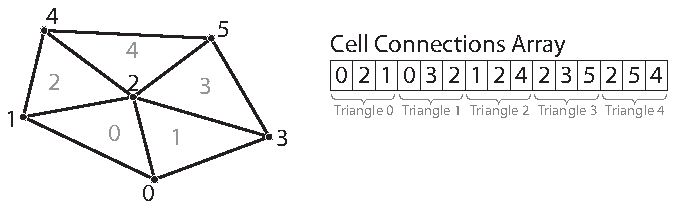
\includegraphics{images/ExplicitCellConnections}
  \caption{An example explicit mesh.}
  \label{fig:ExplicitMesh}
\end{figure}

The \vtkmcont{DataSetBuilderExplicit} class can be used to create data sets
with explicit meshes. \textidentifier{DataSetBuilderExplicit} has several
versions of a method named \textcode{Create}. Generally, these methods take
the shapes, number of indices, and connectivity arrays as well as an array
of point coordinates. These arrays can be given in \textcode{std::vector}
objects, and the data are copied into the \textidentifier{DataSet} created.

The following example creates a mesh like the one shown in
Figure~\ref{fig:ExplicitMesh}.

\vtkmlisting{Creating an explicit mesh with \textidentifier{DataSetBuilderExplicit}.}{CreateExplicitGrid.cxx}

Often it is awkward to build your own arrays and then pass them to
\textidentifier{DataSetBuilderExplicit}. There also exists an alternate
builder class named \vtkmcont{DataSetBuilderExplicitIterative} that allows
you to specify each cell and point one at a time rather than all at once.
This is done by calling one of the versions of \textcode{AddPoint} and one
of the versions of \textcode{AddCell} for each point and cell,
respectively. The next example also builds the mesh shown in
Figure~\ref{fig:ExplicitMesh} except this time using
\textidentifier{DataSetBuilderExplicitIterative}.

\vtkmlisting{Creating an explicit mesh with \textidentifier{DataSetBuilderExplicitIterative}.}{CreateExplicitGridIterative.cxx}

\subsubsection{Add Fields}

In addition to creating the geometric structure of a data set, it is
usually important to add fields to the data. Fields describe numerical data
associated with the topological elements in a cell. They often represent a
physical quantity (such as temperature, mass, or volume fraction) but can
also represent other information (such as indices or classifications).

The easiest way to define fields in a data set is to use the
\vtkmcont{DataSetFieldAdd} class. This class works on
\textidentifier{DataSet}s of any type. It has methods named
\textcode{AddPointField} and \textcode{AddCellField} that define a field
for either points or cells. Every field must have an associated field name.

Both \textcode{AddPointField} and \textcode{AddCellField} are overloaded to
accept arrays of data in different structures. Field arrays can be passed
as standard C arrays or as \textcode{std::vector}s, in which case the data
are copied. Field arrays can also be passed in a
\textidentifier{ArrayHandle}, in which case the data are not copied.

The following (somewhat contrived) example defines fields for a uniform
grid that identify which points and cells are on the boundary of the mesh.

\vtkmlisting{Adding fields to a \textidentifier{DataSet}.}{AddFieldData.cxx}

\index{data~set!Building|)}

\subsection{Cell Sets}
\label{sec:DataSets:CellSets}

\index{cell~set|(}
\index{data~set!cell~set|see{cell~set}}

A cell set determines the topological structure of the data in a data set.
Fundamentally, any cell set is a collection of cells, which typically (but
not always) represent some region in space. 3D cells are made up of points,
edges, and faces. (2D cells have only points and edges, and 1D cells have
only points.) The arrangement of these points, edges, and faces is defined
by the \index{shape}\index{cell~set!shape}\index{cell~shape}\keyterm{shape}
of the cell, which prescribes a specific ordering of each. The basic cell
shapes provided by VTK-m are discussed in detail in
Section~\ref{sec:CellShapeTagsIds} starting on
page~\pageref{sec:CellShapeTagsIds}.

There are multiple ways to express the connections of a cell set, each with
different benefits and restrictions. These different cell set types are
managed by different cell set classes in VTK-m. All VTK-m cell set classes
inherit from \vtkmcont{CellSet}. The two basic types of cell sets are
structured and explicit, and there are several variations of these types.

\subsubsection{Structured Cell Sets}

\index{cell~set!structured|(}
\index{structured~cell~set|(}

A \vtkmcont{CellSetStructured} defines a 1-, 2-, or 3-dimensional grid of
points with lines, quadrilaterals, or hexahedra, respectively, connecting
them. The topology of a \textidentifier{CellSetStructured} is specified by
simply providing the dimensions, which is the number of points in the $i$,
$j$, and $k$ directions of the grid of points. The number of points is
implicitly $i \times j \times k$ and the number of cells is implicitly
$(i-1) \times (j-1) \times (k-1)$ (for 3D grids).
Figure~\ref{fig:CellSetStructured} demonstrates this arrangement.

\begin{figure}
  \centering
  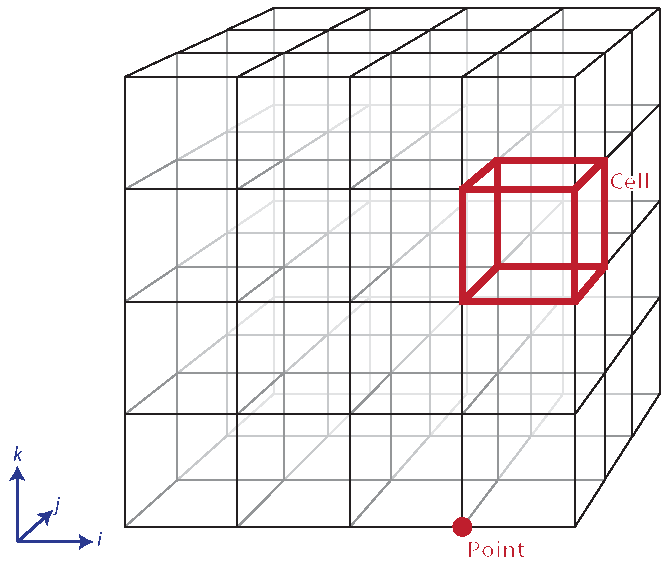
\includegraphics{images/StructuredCellSet}
  \caption{The arrangement of points and cells in a 3D structured grid.}
  \label{fig:CellSetStructured}
\end{figure}

The big advantage of using \vtkmcont{CellSetStructured} to define a cell
set is that it is very space efficient because the entire topology can be
defined by the three integers specifying the dimensions. Also algorithms
can be optimized for \textidentifier{CellSetStructured}'s regular nature.
However, \textidentifier{CellSetStructured}'s strictly regular grid
structure also limits its applicability. A structured cell set can only be
a dense grid of lines, quadrilaterals, or hexahedra. It cannot represent
irregular data well.

Many data models in other software packages, such as the one for VTK, make
a distinction between uniform, rectilinear, and curvilinear grids. VTK-m's
cell sets do not. All three of these grid types are represented by
\textidentifier{CellSetStructured}. This is because in a VTK-m data set the
cell set and the coordinate system are defined independently and used
interchangeably. A structured cell set with uniform point coordinates makes
a uniform grid. A structured cell set with point coordinates defined
irregularly along coordinate axes makes a rectilinear grid. And a
structured cell set with arbitrary point coordinates makes a curvilinear
grid. The point coordinates are defined by the data set's coordinate system,
which is discussed in Section~\ref{sec:DataSets:CoordinateSystems} starting
on page~\pageref{sec:DataSets:CoordinateSystems}.

\index{structured~cell~set|)}
\index{cell~set!structured|)}

\subsubsection{Explicit Cell Sets}

\index{explicit~cell~set|(}
\index{cell~set!explicit|(}

A \vtkmcont{CellSetExplicit} defines an irregular collection of cells. The
cells can be of different types and connected in arbitrary ways. This is
done by explicitly providing for each cell a sequence of points that
defines the cell.

An explicit cell set is defined with a minimum of three arrays. The first
array identifies the shape of each cell. (Cell shapes are discussed in
detail in Section~\ref{sec:CellShapeTagsIds} starting on
page~\pageref{sec:CellShapeTagsIds}.) The second array identifies how many
points are in each cell. The third array has a sequence of point indices
that make up each cell. Figure~\ref{fig:CellSetExplicit} shows a simple
example of an explicit cell set.

\begin{figure}
  \centering
  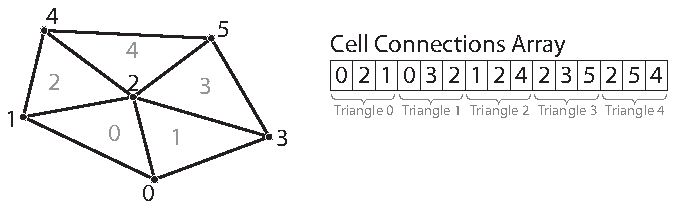
\includegraphics{images/ExplicitCellConnections}
  \caption{Example of cells in a \textidentifier{CellSetExplict} and the
    arrays that define them.}
  \label{fig:CellSetExplicit}
\end{figure}

An explicit cell set may also have other topological arrays such as an
array of offsets of each cell into the connectivity array or an array of
cells incident on each point. Although these arrays can be provided, they
are optional and can be internally derived from the shape, num indices, and
connectivity arrays.

\vtkmcont{ExplicitCellSet} is a powerful representation for a cell set
because it can represent an arbitrary collection of cells. However, because
all connections must be explicitly defined,
\textidentifier{ExplicitCellSet} requires a significant amount of memory to
represent the topology.

\index{cell~set!single~type|(}
\index{explicit~cell~set!single~type|(}
\index{single~type~cell~set|(}

An important specialization of an explicit cell set is
\vtkmcont{CellSetSingleType}. \textidentifier{CellSetSingleType} is an
explicit cell set constrained to contain cells that all have the same shape
and all have the same number of points. So for example if you are creating
a surface that you know will contain only triangles,
\textidentifier{CellSetSingleType} is a good representation for these data.

Using \textidentifier{CellSetSingleType} saves memory because the array of
cell shapes and the array of point counts no longer need to be stored.
\textidentifier{CellSetSingleType} also allows VTK-m to skip some
processing and other storage required for general explicit cell sets.

\index{single~type~cell~set|)}
\index{explicit~cell~set!single~type|)}
\index{cell~set!single~type|)}

\index{cell~set!explicit|)}
\index{explicit~cell~set|)}

\subsubsection{Cell Set Permutations}

\index{permutation~cell~set|(}
\index{cell~set!permutation|(}

A \vtkmcont{CellSetPermutation} rearranges the cells of one cell set to
create another cell set. This restructuring of cells is not done by copying
data to a new structure. Rather, \textidentifier{CellSetPermutation}
establishes a look-up from one cell structure to another. Cells are permuted
on the fly while algorithms are run.

A \textidentifier{CellSetPermutation} is established by providing a mapping
array that for every cell index provides the equivalent cell index in the
cell set being permuted. \textidentifier{CellSetPermutation} is most often
used to mask out cells in a data set so that algorithms will skip over
those cells when running. Note that although
\textidentifier{CellSetPermutation} can mask cells, it cannot mask points.
All points from the original cell set are available in the permuted cell
set regardless of whether they are used.

The following example uses \vtkmcont{CellSetPermutation} with a counting
array to expose every tenth cell. This provides a simple way to subsample a
data set.

\vtkmlisting{Subsampling a data set with \textidentifier{CellSetPermutation}.}{CreateCellSetPermutation.cxx}

\index{cell~set!permutation|)}
\index{permutation~cell~set|)}

\subsubsection{Dynamic Cell Sets}

\index{dynamic~cell~set|(}
\index{cell~set!dynamic|(}

\vtkmcont{DataSet} must hold an arbitrary collection of \vtkmcont{CellSet}
objects, which it cannot do while knowing their types at compile time. To
manage storing \textidentifier{CellSet}s without knowing their types,
\textidentifier{DataSet} actually holds references using
\vtkmcont{DynamicCellSet}.

\textidentifier{DynamicCellSet} is similar in nature to
\textidentifier{DynamicArrayHandle} except that it, of course, holds
\textidentifier{CellSet}s instead of \textidentifier{ArrayHandle}s. The
interface for the two classes is similar, and you should review the
documentation for \textidentifier{DynamicArrayHandle} (in
Section~\ref{sec:DynamicArrayHandle} starting on
page~\pageref{sec:DynamicArrayHandle}) to understand
\textidentifier{DynamicCellSet}.

\vtkmcont{DynamicCellSet} has a method named \textcode{GetCellSet} that
returns a const reference to the held cell set as the abstract
\textidentifier{CellSet} class. This can be used to easily access the
virtual methods in the \textidentifier{CellSet} interface. You can also
create a new instance of a cell set with the same type using the
\textcode{NewInstance} method.

The \textidentifier{DynamicCellSet}\textcode{::IsType()} method can be used
to determine whether the cell set held in the dynamic cell set is of a
given type. If the cell set type is known,
\textidentifier{DynamicCellSet}\textcode{::CastTo()} can be used to safely
downcast the cell set object.

When a typed version of the cell set stored in the
\textidentifier{DynamicCellSet} is needed but the type is not known, which
happens regularly in the internal workings of VTK-m, the
\textcode{CastAndCall} method can be used to make this transition.
\textcode{CastAndCall} works by taking a functor and calls it with the
appropriately cast cell set object.

The \textcode{CastAndCall} method works by attempting to cast to a known
set of types. This set of types used is defined by the macro
\vtkmmacro{VTKM\_DEFAULT\_CELL\_SET\_LIST\_TAG}, which is declared in
\vtkmheader{vtkm/cont}{CellSetListTag.h}. This list can be overridden
globally by defining the \vtkmmacro{VTKM\_DEFAULT\_CELL\_SET\_LIST\_TAG}
macro \emph{before} any VTK-m headers are included.

The set of types used in a \textcode{CastAndCall} can also be changed only
for a particular instance of a dynamic cell set by calling its
\textcode{ResetCellSetList}. This method takes a list of cell types and
returns a new dynamic array handle of a slightly different type that will
use this new list of cells for dynamic casting.

\index{cell~set!dynamic|)}
\index{dynamic~cell~set|}

\subsubsection{Blocks and Assemblies}

Rather than just one cell set, a \vtkmcont{DataSet} can hold multiple cell
sets. This can be used to construct multiblock data structures or
assemblies of parts. Multiple cell sets can also be used to represent
subsets of the data with particular properties such as all cells filled
with a material of a certain type. Or these multiple cells might represent
particular features in the data, such as the set of faces representing a
boundary in the simulation.

\subsubsection{Zero Cell Sets}

It is also possible to construct a \vtkmcont{DataSet} that contains no cell
set objects whatsoever. This can be used to manage data that does not
contain any topological structure. For example, a collection of series that
come from columns in a table could be stored as multiple fields in a data
set with no cell set.

\index{cell~set|)}

\subsection{Fields}
\label{sec:DataSets:Fields}

\index{field|(}
\index{data~set!field|see{field}}

A field on a data set provides a value on every point in space on the mesh.
Fields are often used to describe physical properties such as pressure,
temperature, mass, velocity, and much more. Fields are represented in a
VTK-m data set as an array where each value is associated with a particular
element type of a mesh (such as points or cells). This association of field
values to mesh elements and the structure of the cell set determines how
the field is interpolated throughout the space of the mesh.

Fields are manged by the \vtkmcont{Field} class. \textidentifier{Field}
holds its data with a \textidentifier{DynamicArrayHandle}, which itself is
a container for an \textidentifier{ArrayHandle}. \textidentifier{Field}
also maintains the association and, optionally, the name of a cell set for
which the field is valid.

The data array can be retrieved as a \textidentifier{DynamicArrayHandle}
using the \textcode{GetData} method of \textidentifier{Field}.
\textidentifier{Field} also has a convenience method named
\textcode{GetBounds} that finds the range of values stored in the field
array.

\index{field|}

\subsection{Coordinate Systems}
\label{sec:DataSets:CoordinateSystems}

\index{coordinate~system|(}
\index{data~set!coordinate~system|see{coordinate~system}}

A coordinate system determines the location of a mesh's elements in space.
The spatial location is described by providing a 3D vector at each point
that gives the coordinates there. The point coordinates can then be
interpolated throughout the mesh.

Coordinate systems are managed by the \vtkmcont{CoordinateSystem} class. In
actuality, a coordinate system is just a field with a special meaning, and
so the \textidentifier{CoordinateSystem} class inherits from the
\textidentifier{Field} class. \textidentifier{CoordinateSystem} constrains
the field to be associated with points and typically has 3D floating point
vectors for values.

It is typical for a \textidentifier{DataSet} to have one coordinate system
defined, but it is possible to define multiple coordinate systems. This is
helpful when there are multiple ways to express coordinates. For example,
positions in geographic may be expressed as Cartesian coordinates or as
latitude-longitude coordinates. Both are valid and useful in different
ways.

It is also valid to have a \textidentifier{DataSet} with no coordinate
system. This is useful when the structure is not rooted in physical space.
For example, if the cell set is representing a graph structure, there might
not be any physical space that has meaning for the graph.

\index{coordinate~system|)}

\index{data~set|)}

\section{Timers}
\label{sec:Timers}

\index{timer|(}

It is often the case that you need to measure the time it takes for an
operation to happen. This could be for performing measurements for
algorithm study or it could be to dynamically adjust scheduling.

Performing timing in a multi-threaded environment can be tricky because
operations happen asynchronously. In the VTK-m control environment timing
is simplified because the control environment operates on a single
thread. However, operations invoked in the execution environment may run
asynchronously to operations in the control environment.

To ensure that accurate timings can be made, VTK-m provides a
\vtkmcont{Timer} class that is templated on the device adapter to provide
an accurate measurement of operations that happen on the device. If not
template parameter is provided, the default device adapter is used.

The timing starts when the \textidentifier{Timer} is constructed. The time
elapsed can be retrieved with a call to the \textcode{GetElapsedTime}
method. This method will block until all operations in the execution
environment complete so as to return an accurate time. The timer can be
restarted with a call to the \textcode{Reset} method.

\fix{This example needs to be updated when something interesting can be
  invoked.}

\vtkmlisting{Using \protect\vtkmcont{Timer}.}{Timer.cxx}

\index{timer|)}

\section{Error Handling}
\label{sec:ErrorHandlingControl}

\index{errors|(}

VTK-m uses exceptions to report errors. All exceptions thrown by VTK-m will
be a subclass of \vtkmcont{Error}. For simple error reporting, it is
possible to simply catch a \vtkmcont{Error} and report the error message
string reported by the \textcode{GetMessage} method.

\vtkmlisting{Simple error reporting.}{CatchingErrors.cxx}

There are several subclasses to \vtkmcont{Error}. The specific subclass
gives an indication of the type of error that occured when the exception
was thrown. Catching one of these subclasses may help a program better
recover from errors.
\begin{description}
\item[\vtkmcont{ErrorControlAssert}] \index{assert} \index{errors!assert}
  Thrown when an assertion fails, meaning a VTK-m operation reached an
  unexpected state. The header file \vtkmheader{vtkm/cont}{Assert.h}
  defines a macro named \vtkmmacro{VTKM\_ASSERT\_CONT} that behaves much
  like the POSIX C assert macro except that a
  \textidentifier{ErrorControlAssert} is thrown rather than killing the
  application outright.
\item[\vtkmcont{ErrorControlBadAllocation}] Thrown when there is a problem
  accessing or manipulating memory. Often this is thrown when an allocation
  fails because there is insufficient memory, but other memory access
  errors can cause this to be thrown as well.
\item[\vtkmcont{ErrorControlBadType}] Thrown when VTK-m attempts to perform
  an operation on an object that is of an incompatible type.
\item[\vtkmcont{ErrorControlBadValue}] Thrown when a VTK-m function or
  method encounters an invalid value that inhibits progress.
\item[\vtkmcont{ErrorExecution}] \index{errors!execution~environment} Throw
  when an error is signaled in the execution environment for example when a
  worklet is being executed.
\item[\vtkmcont{ErrorControlInternal}] Thrown when VTK-m detects an
  internal state that should never be reached. This error usually indicates
  a bug in VTK-m or, at best, VTK-m failed to detect an invalid input it
  should have.
\item[\vtkmio{ErrorIO}] Thrown by a reader or writer when a file error is
  encountered.
\end{description}

\index{errors|)}

\index{environment!control|)}
\index{control~environment|)}



\chapter{Execution Environment}
\label{chap:ExecutionEnvironment}

\fix{Write this.}

% -*- latex -*-

\chapter{Worklets}
\label{chap:Worklets}

\index{worklet|(}

The simplest way to implement an algorithm in VTK-m is to create a
\keyterm{worklet}. A worklet is fundamentally a functor that operates on an
element of data. Thus, it is a \textcode{class} or \textcode{struct} that
has an overloaded parenthesis operator (which must be declared
\textcode{const} for thread safety). However, worklets are also embedded
with a significant amount of metadata on how the data should be managed and
how the execution should be structured. This chapter explains the basic
mechanics of defining and using worklets.


\section{Worklet Types}
\label{sec:WorkletTypes}

\index{worklet~types|(}

Different operations in visualization can have different data access
patterns, perform different execution flow, and require different
provisions. VTK-m manages these different accesses, execution, and
provisions by grouping visualization algorithms into common classes of
operation and supporting each class with its own worklet type.

Each worklet type has a generic superclass that worklets of that particular
type must inherit. This makes the type of the worklet easy to identify. The
following list describes each worklet type provided by VTK-m and the
superclass that supports it. Details on how to create worklets of each type
are given in Section~\ref{sec:WorkletTypeReference}. It is also possible
to create new worklet types in VTK-m. This is an advanced topic covered in
Chapter~\ref{chap:AdvancedWorklets}.

\begin{description}
\item[Field Map] \index{worklet~types!field~map} \index{field~map~worklet}
  A worklet deriving \vtkmworklet{WorkletMapField} performs a basic mapping
  operation that applies a function (the operator in the worklet) on all
  the field values at a single point or cell and creates a new field value
  at that same location. Although the intention is to operate on some
  variable over a mesh, a \textidentifier{WorkletMapField} may actually be
  applied to any array. Thus, a field map can be used as a basic
  \index{map}map operation.

\item[Topology Map] \index{worklet~types!topology~map}
  \index{topology~map~worklet} A worklet deriving
  \vtkmworklet{WorkletMapTopology} or one of its sibling classes performs a
  mapping operation that applies a function (the operator in the worklet)
  on all elements of a particular type (such as points or cells) and
  creates a new field for those elements. The basic operation is similar to
  a field map except that in addition to access fields being mapped on, the
  worklet operation also has access to incident fields.

  There are multiple convenience classes available for the most common
  types of topology mapping. \index{worklet~types!point~to~cell}
  \index{point~to~cell~worklet} \vtkmworklet{WorkletMapPointToCell} calls
  the worklet operation for each cell and makes every incident point
  available. This type of map also has access to cell structures and can
  interpolate point fields.
  %% \index{worklet~types!cell~to~point}
  %% \index{cell~to~point~worklet} \vtkmworklet{WorkletMapCellToPoint} calls
  %% the worklet operation for each point and makes every incident cell
  %% available.
\end{description}

\index{worklet~types|)}


\section{Dispatchers}
\label{sec:Dispatchers}

\index{dispatcher|(}

Worklets, both those provided by VTK-m as listed in
Section~\ref{sec:ProvidedWorklets} and ones created by a user as described
in Section~\ref{sec:CreatingWorklets}, are instantiated in the control
environment and run in the execution environment. This means that the
control environment must have a means to \index{invoke}\keyterm{invoke}
worklets that start running in the execution environment.

This invocation is done through a set of
\index{dispatcher}\keyterm{dispatcher} objects. A dispatcher object is an
object in the control environment that has an instance of a worklet and can
invoke that worklet with a set of arguments. There are multiple types of
dispatcher objects, each corresponding to a type of worklet object. All
dispatcher objects have at least two template parameters: the worklet class
being invoked, which is always the first argument, and the device adapter
tag, which is always the last argument and will be set to the default
device adapter if not specified.

All dispatcher classes have a method named \textcode{Invoke} that launches
the worklet in the execution environment.  The arguments to
\textcode{Invoke} must match those expected by the worklet, which is
specified by something called a \keyterm{control signature}. The expected
arguments for worklets provided by VTK-m are documented in
Section~\ref{sec:ProvidedWorklets}. Also, for any worklet, the
\textcode{Invoke} arguments can be gleaned from the control signature,
which is described in Section~\ref{sec:ControlSignature}.

The following is a list of the dispatchers defined in VTK-m. The
dispatcher classes correspond to the list of worklet types specified in
Section~\ref{sec:WorkletTypes}. Many examples of using these dispatchers
are provided in Section~\ref{sec:ProvidedWorklets}.

\begin{description}
\item[\vtkmworklet{DispatcherMapField}] The dispatcher used in conjunction
  with a worklet that subclasses \vtkmworklet{WorkletMapField}. The
  dispatcher class has two template arguments: the worklet type and the
  device adapter (optional).
\item[\vtkmworklet{DispatcherMapTopology}] The dispatcher used in
  conjunction with a worklet that subclasses
  \vtkmworklet{WorkletMapTopology} or one of its sibling classes (such as
  \vtkmworklet{WorkletMapPointToCell}). The dispatcher class has two
  template arguments: the worklet type and the device adapter (optional).
%% \item[\daxcont{DispatcherMapCell}] The dispatcher used in conjunction with
%%   a worklet that subclasses \dax{WorkletMapCell}. The class has two
%%   template arguments: the worklet type and the device adapter (optional).
%% \item[\daxcont{DispatcherGenerateTopology}] The dispatcher used in
%%   conjunction with a worklet that subclasses
%%   \dax{WorkletGenerateTopology}. The class has three template arguments: the
%%   worklet type, the type of array handle containing the count of the number
%%   of cells being generated (optional), and the device adapter
%%   (optional). The default type of the count array handle is
%%   \daxcont{ArrayHandle}\textcode{<}\dax{Id}\textcode{>}. An instance of the
%%   count array handle must be provided in the constructor of
%%   \daxcont{DispatcherGenerateTopology}.
%% \item[\daxcont{DispatcherInterpolatedCell}] The dispatcher used in
%%   conjunction with a worklet that subclasses
%%   \dax{WorkletInterpolatedCell}. The class has three template arguments: the
%%   worklet type, the type of array handle containing the count of the number
%%   of cells being generated (optional), and the device adapter
%%   (optional). The default type of the count array handle is
%%   \daxcont{ArrayHandle}\textcode{<}\dax{Id}\textcode{>}. An instance of the
%%   count array handle must be provided in the constructor of
%%   \daxcont{DispatcherInterpolatedCell}.
%% \item[\daxcont{DispatcherGenerateKeysValues}] The dispatcher used in
%%   conjunction with a worklet that subclasses
%%   \dax{WorkletGenerateKeysValues}. The class has three template arguments:
%%   the worklet type, the type of array handle containing the count of the
%%   number of key-values being generated (optional), and the device adapter
%%   (optional). The default type of the count array handle is
%%   \daxcont{ArrayHandle}\textcode{<}\dax{Id}\textcode{>}. An instance of the
%%   count array handle must be provided in the constructor of
%%   \daxcont{DispatcherGenerateKeysValues}.
%% \item[\daxcont{DispatcherReduceKeysValues}] The dispatcher used in
%%   conjunction with a worklet that subclasses
%%   \dax{WorkletReduceKeysValues}. The class has three template arguments:
%%   the worklet type, the type of array handle containing the keys
%%   (optional), and the device adapter (optional). The default type of the
%%   key array handle is
%%   \daxcont{ArrayHandle}\textcode{<}\dax{Id}\textcode{>}. An instance of the
%%   key array handle must be provided in the constructor of
%%   \daxcont{DispatcherReduceKeysValues}.
\end{description}

\index{dispatcher|)}

\section{Provided Worklets}
\label{sec:ProvidedWorklets}

\VTKm comes with several worklet implementations.
These worklet implementations for the most part provide the underlying implementations of the filters described in Chapter~\ref{chap:ProvidedFilters}.
The easiest way to execute a filter is to run it from the associated filter class.
However, if your data is not in a \vtkmcont{DataSet} structure or you have knowledge of the specific data types used in the \textidentifier{DataSet}, it might be more efficient to run the worklet directly.
Note that many of the filters use multiple worklets under the covers to implement the full functionality.

The following example demonstrates using the simple \vtkmworklet{PointElevation} worklet directly.

\vtkmlisting{Using the provided \textidentifier{PointElevation} worklet.}{UsePointElevationWorklet.cxx}


\section{Creating Worklets}
\label{sec:CreatingWorklets}

\index{worklet!creating|(}

A worklet is created by implementing a \textcode{class} or
\textcode{struct} with the following features.

\begin{enumerate}
\item The class must contain a \controlsignature \textcode{typedef}, which
  specifies what arguments are expected when invoking the class with a
  dispatcher in the control environment.
\item The class must contain an \executionsignature \textcode{typedef},
  which specifies how the data gets passed from the arguments in the
  control environment to the worklet running in the execution environment.
\item The class must contain an \inputdomain \textcode{typedef}, which
  identifies which input parameter defines the input domain of the data.
\item The class may define a scatter operation to override a 1:1 mapping
  from input to output.
\item The class must contain an overload of the parenthesis operator, which
  is the method that is executed in the execution environment.
\item The class must publicly inherit from a base worklet class that
  specifies the type of operation being performed.
\end{enumerate}

Figure~\ref{fig:WorkletExampleAnnotated} demonstrates all of the required
components of a worklet.

%% \pagebreak
%% \begin{vtkmexample}{Example Code for Cutting/Pasting.}
%% class TriangulateCell : public vtkm::worklet::WorkletMapPointToCell
%% {
%% public:
%%   typedef void ControlSignature(CellSetIn topology,
%%                                 ExecObject tables,
%%                                 FieldOutCell<> connectivityOut);
%%   typedef void ExecutionSignature(CellShape, PointIndices, _2, _3, VisitIndex);
%%   typedef _1 InputDomain;

%%   typedef vtkm::worklet::ScatterCounting ScatterType;
%%   VTKM_CONT
%%   ScatterType GetScatter() const
%%   {
%%     return this->Scatter;
%%   }

%%   template<typename CellShapeTag,
%%            typename ConnectivityInVec,
%%            typename ConnectivityOutVec>
%%   VTKM_EXEC
%%   void operator()(
%%       CellShapeTag shape,
%%       const ConnectivityInVec &connectivityIn,
%%       const internal::TriangulateTablesExecutionObject<DeviceAdapter> &tables,
%%       ConnectivityOutVec &connectivityOut,
%%       vtkm::IdComponent visitIndex) const
%%   {
%% \end{vtkmexample}
%% \pagebreak

\begin{figure}[htb]
  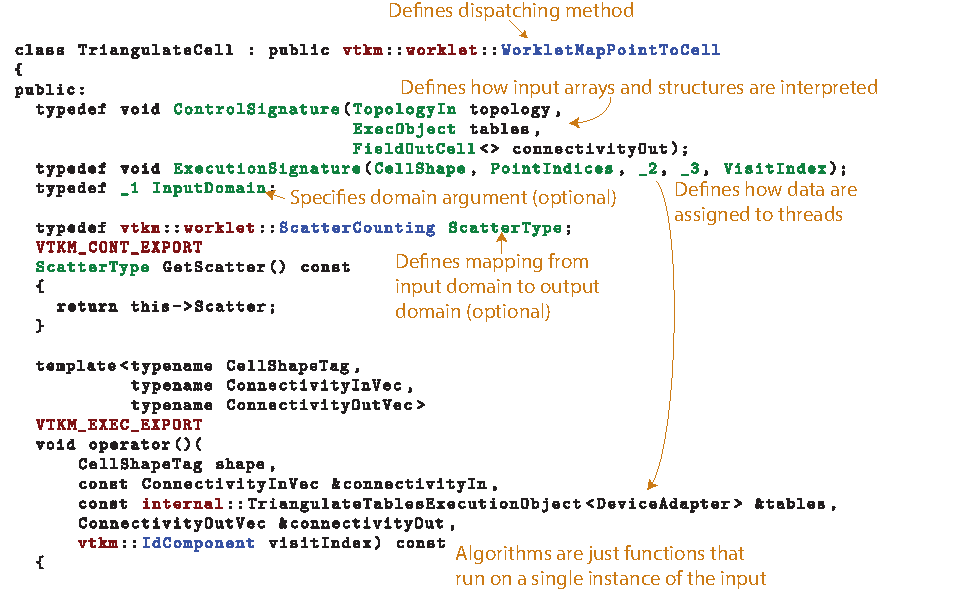
\includegraphics[width=\linewidth]{images/WorkletExampleAnnotated}
  \caption{Annotated example of a worklet declaration.}
  \label{fig:WorkletExampleAnnotated}
\end{figure}

\subsection{Control Signature}
\label{sec:ControlSignature}

\index{control~signature|(}
\index{signature!control|(}
\index{worklet!control~signature|(}

The control signature of a worklet is the \textcode{typedef} of a function
prototype named \controlsignature. The function prototype matches the
calling specification used with the dispatcher \textcode{Invoke} function.

\vtkmlisting{A \protect\controlsignature.}{ControlSignature.cxx}

The return type of the function prototype is always \textcode{void} because
the dispatcher \textcode{Invoke} functions do not return values. The
parameters of the function prototype are \index{signature tags}\keyterm{tags}
that identify the type of data that is expected to be passed to invoke.
\controlsignature tags are defined by the worklet type and the various tags
are documented more fully in Section~\ref{sec:WorkletTypeReference}.

By convention, \controlsignature tag names start with the base concept
(e.g. \textsignature{Field} or \textsignature{Topology}) followed by the
domain (e.g. \textsignature{Point} or \textsignature{Cell}) followed by
\textsignature{In} or \textsignature{Out}. For example,
\sigtag{FieldPointIn} would specify values for a field on the points of a
mesh that are used as input (read only). Although they should be there in
most cases, some tag names might leave out the domain or in/out parts if
they are obvious or ambiguous.

\subsubsection{Type List Tags}
\label{sec:TypeListTags}

\index{type~list~tags|(}
\index{control~signature!type~list~tags|(}

Some tags are templated to have modifiers. For example,
\textsignature{Field} tags have a template argument that is set to a type
list tag defining what types of field data are supported. (See
Section~\ref{sec:TypeLists} for a description of type lists.) In fact, this
type list modifier is so common that the following convenience subtags used
with \textsignature{Field} tags are defined for all worklet types.

\begin{didyouknow}
  Any type list will work as modifiers for \controlsignature tags. However,
  these common type lists are provided for convenience and to make the
  \controlsignature shorter and more readable.
\end{didyouknow}

\begin{description}
  \label{TypeTagList}
\item[\sigtag{AllTypes}] All possible types.
\item[\sigtag{CommonTypes}] The most used types in visualization. This
  includes signed integers and floats that are 32 or 64 bit. It also
  includes 3 dimensional vectors of floats. The same as
  \vtkm{TypeListTagCommon}.
\item[\sigtag{IdType}] Contains the single item \vtkm{Id}. The same as
  \vtkm{TypeListTagId}.
\item[\sigtag{Id2Type}] Contains the single item \vtkm{Id2}. The same as
  \vtkm{TypeListTagId2}.
\item[\sigtag{Id3Type}] Contains the single item \vtkm{Id3}. The same as
  \vtkm{TypeListTagId3}.
\item[\sigtag{Index}] All types used to index arrays. Contains \vtkm{Id},
  \vtkm{Id2}, and \vtkm{Id3}. The same as \vtkm{TypeListTagIndex}.
\item[\sigtag{FieldCommon}] A list containing all the types generally
  used for fields. It is the combination of \sigtag{Scalar}, \sigtag{Vec2},
  \sigtag{Vec3}, and \sigtag{Vec4}. The same as \vtkm{TypeListTagField}.
\item[\sigtag{Scalar}] Types used for scalar fields. Specifically, it
  contains floating point numbers of different widths (i.e. \vtkm{Float32}
  and \vtkm{Float64}). The same as \vtkm{TypeListTagFieldScalar}.
\item[\sigtag{ScalarAll}] All scalar types. It contains signed and unsigned
  integers of widths from 8 to 64 bits. It also contains floats of 32 and
  64 bit widths. The same as \vtkm{TypeListTagScalarAll}.
\item[\sigtag{Vec2}] Types for values of fields with 2 dimensional
  vectors. All these vectors use floating point numbers. The same as
  \vtkm{TypeListTagFieldVec2}.
\item[\sigtag{Vec3}] Types for values of fields with 3 dimensional
  vectors. All these vectors use floating point numbers. The same as
  \vtkm{TypeListTagFieldVec3}.
\item[\sigtag{Vec4}] Types for values of fields with 4 dimensional
  vectors. All these vectors use floating point numbers. The same as
  \vtkm{TypeListTagFieldVec4}.
\item[\sigtag{VecAll}] All \vtkm{Vec} classes with standard integers or
  floating points as components and lengths between 2 and 4. The same as
  \vtkm{TypeListTagVecAll}.
\item[\sigtag{VecCommon}] The most common vector types. It contains all
  \vtkm{Vec} class of size 2 through 4 containing components of unsigned
  bytes, signed 32-bit integers, signed 64-bit integers, 32-bit floats, or
  64-bit floats. The same as \vtkm{TypeListTagVecCommon}.
\end{description}

\index{control~signature!type~list~tags|)}
\index{type~list~tags|)}

\index{worklet!control~signature|)}
\index{signature!control|)}
\index{control~signature|)}

\subsection{Execution Signature}
\label{sec:ExecutionSignature}

\index{execution~signature|(}
\index{signature!execution|(}
\index{worklet!execution~signature|(}

Like the control signature, the execution signature of a worklet is the
\textcode{typedef} of a function prototype named \executionsignature. The
function prototype must match the parenthesis operator (described in
Section~\ref{sec:WorkletOperator}) in terms of arity and argument
semantics.

\vtkmlisting{An \protect\executionsignature.}{ExecutionSignature.cxx}

The arguments of the \executionsignature's function prototype are tags that
define where the data come from. The most common tags are an underscore
followed by a number, such as \sigtagnum{1}, \sigtagnum{2}, etc. These
numbers refer back to the corresponding argument in the
\controlsignature. For example, \sigtagnum{1} means data from the first
control signature argument, \sigtagnum{2} means data from the second
control signature argument, etc.

Unlike the control signature, the execution signature optionally can
declare a return type if the parenthesis operator returns a value. If this
is the case, the return value should be one of the numeric tags
(i.e. \sigtagnum{1}, \sigtagnum{2}, etc.) to refer to one of the data
structures of the control signature. If the parenthesis operator does not
return a value, then \executionsignature should declare the return type as
\textcode{void}.

In addition to the numeric tags, there are other execution signature tags
to represent other types of data. For example, the \sigtag{WorkIndex} tag
identifies the instance of the worklet invocation. Each call to the worklet
function will have a unique \sigtag{WorkIndex}. Other such tags exist and
are described in the following section on worklet types where appropriate.

\index{worklet!execution~signature|)}
\index{signature!execution|)}
\index{execution~signature|)}

\subsection{Input Domain}
\label{sec:InputDomain}

\index{input domain|(}
\index{worklet!input~domain|(}

All worklets represent data parallel operations that are executed over
independent elements in some domain. The type of domain is inherent from
the worklet type, but the size of the domain is dependent on the data being
operated on. One of the arguments given to the dispatcher's
\textcode{Invoke} in the control environment must specify the domain.

A worklet identifies the argument specifying the domain with a
\textcode{typedef} named \inputdomain. The \inputdomain must be
\textcode{typedef}ed to one of the execution signature numeric tags
(i.e. \sigtagnum{1}, \sigtagnum{2}, etc.). By default, the \inputdomain
points to the first argument, but a worklet can override that to point to
any argument.

\vtkmlisting{An \protect\inputdomain declaration.}{InputDomain.cxx}

Different types of worklets can have different types of domain. For example
a simple field map worklet has a \sigtag{FieldIn} argument as its input
domain, and the size of the input domain is taken from the size of the
associated field array. Likewise, a worklet that maps topology has a
\sigtag{CellSetIn} argument as its input domain, and the size of the input
domain is taken from the cell set.

Specifying the \inputdomain is optional. If it is not specified, the first
argument is assumed to be the input domain.

\index{worklet!input~domain|)}
\index{input domain|)}

\subsection{Worklet Operator}
\label{sec:WorkletOperator}

A worklet is fundamentally a functor that operates on an element of data.
Thus, the algorithm that the worklet represents is contained in or called
from the parenthesis operator method.

\vtkmlisting{An overloaded parenthesis operator of a worklet.}{WorkletOperator.cxx}

There are some constraints on the parenthesis operator. First, it must have
the same arity as the \executionsignature, and the types of the parameters
and return must be compatible. Second, because it runs in the execution
environment, it must be declared with the \vtkmexecmodifier (or
\vtkmexeccontmodifier) modifier. Third, the method must be declared
\textcode{const} to help preserve thread safety.

\section{Worklet Type Reference}
\label{sec:WorkletTypeReference}

\index{worklet~types|(}

There are multiple worklet types provided by VTK-m, each designed to
support a particular type of operation. Section~\ref{sec:WorkletTypes} gave
a brief overview of each type of worklet. This section gives a much more
detailed reference for each of the worklet types including identifying the
generic superclass that a worklet instance should derive, listing the
signature tags and their meanings, and giving an example of the worklet in
use.

\newcommand{\commoncontrolsignaturetags}{
\item[\sigtag{WholeArrayIn}] This tag represents an array where all entries
  can be read by every worklet invocation. A \sigtag{WholeArrayIn} argument
  expects an \textidentifier{ArrayHandle} in the associated parameter of
  the dispatcher's \textcode{Invoke}. An array portal capable of reading
  from any place in the array is given to the worklet. Whole arrays are
  discussed in detail in Section~\ref{sec:WholeArrays} starting on
  page~\pageref{sec:WholeArrays}.

  \sigtag{WholeArrayIn} has a single template parameter that specifies what
  data types are acceptable for the array. The type tags are described in
  Section~\ref{sec:TypeListTags} starting on page~\pageref{TypeTagList}.

\item[\sigtag{WholeArrayOut}] This tag represents an array where any entry
  can be written by any worklet invocation. A \sigtag{WholeArrayOut}
  argument expects an \textidentifier{ArrayHandle} in the associated
  parameter of the dispatcher's \textcode{Invoke}. An array portal capable
  of writing to any place in the array is given to the worklet. Developers
  should take care when using writable whole arrays as introducing race
  conditions is possible. Whole arrays are discussed in detail in
  Section~\ref{sec:WholeArrays} starting on page~\pageref{sec:WholeArrays}.

  \sigtag{WholeArrayOut} has a single template parameter that specifies
  what data types are acceptable for the array. The type tags are described
  in Section~\ref{sec:TypeListTags} starting on page~\pageref{TypeTagList}.

\item[\sigtag{WholeArrayInOut}] This tag represents an array where any
  entry can be read or written by any worklet invocation. A
  \sigtag{WholeArrayInOut} argument expects an \textidentifier{ArrayHandle}
  in the associated parameter of the dispatcher's \textcode{Invoke}. An
  array portal capable of reading from or writing to any place in the array
  is given to the worklet. Developers should take care when using writable
  whole arrays as introducing race conditions is possible. Whole arrays are
  discussed in detail in Section~\ref{sec:WholeArrays} starting on
  page~\pageref{sec:WholeArrays}.

  \sigtag{WholeArrayInOut} has a single template parameter that specifies
  what data types are acceptable for the array. The type tags are described
  in Section~\ref{sec:TypeListTags} starting on page~\pageref{TypeTagList}.

\item[\sigtag{AtomicArrayInOut}]
  This tag represents an array where any entry can be read or written by any worklet invocation.
  A \sigtag{AtomicArrayInOut} argument expects an \textidentifier{ArrayHandle} in the associated parameter of the dispatcher's \textcode{Invoke}.
  A \vtkmexec{AtomicArray} object capable of performing atomic operations to the entries in the array is given to the worklet.
  Atomic arrays can help avoid race conditions but can slow down the running of a parallel algorithm.
  Atomic arrays are discussed in detail in Section~\ref{sec:AtomicArrays} starting on page~\pageref{sec:AtomicArrays}.

\item[\sigtag{ExecObject}] This tag represents an execution object that is
  passed directly from the control environment to the worklet. A
  \sigtag{ExecObject} argument expects a subclass of
  \vtkmexec{ExecutionObjectBase}, and this same object is given to the
  worklet. Execution objects are discussed in detail in
  Section~\ref{sec:ExecutionObjects} starting on
  page~\pageref{sec:ExecutionObjects}.
}

\newcommand{\numericexecutionsignaturetags}{
\item[\sigtagnum{1}, \sigtagnum{2},$\ldots$] These reference the
  corresponding parameter in the \controlsignature.
}

\newcommand{\commonexecutionsignaturetags}{
\item[\sigtag{WorkIndex}]
  This tag produces a \vtkm{Id} that uniquely identifies the invocation of the worklet.
\item[\sigtag{VisitIndex}]
  This tag produces a \vtkm{IdComponent} that uniquely identifies when multiple worklet invocations operate on the same input item, which can happen when defining a worklet with scatter (as described in Section~\ref{sec:WorkletScatter}).
\item[\sigtag{InputIndex}]
  This tag produces a \vtkm{Id} that identifies the index of the input element, which can differ from the \sigtag{WorkIndex} in a worklet with a scatter (as described in Section~\ref{sec:WorkletScatter}).
\item[\sigtag{OutputIndex}]
  This tag produces a \vtkm{Id} that identifies the index of the output element. (This is generally the same as \sigtag{WorkIndex}.)
}

\subsection{Field Map}

\index{worklet~types!field~map|(}
\index{field~map~worklet|(}
\index{map~field|(}

A worklet deriving \vtkmworklet{WorkletMapField} performs a basic mapping
operation that applies a function (the operator in the worklet) on all the
field values at a single point or cell and creates a new field value at
that same location. Although the intention is to operate on some variable
over the mesh, a \textidentifier{WorkletMapField} can actually be applied
to any array.

A \textidentifier{WorkletMapField} subclass is invoked with a
\vtkmworklet{DispatcherMapField}. This dispatcher has two template
arguments. The first argument is the type of the worklet subclass. The
second argument, which is optional, is a device adapter tag.

A field map worklet supports the following tags in the parameters of its
\controlsignature.

\begin{description}
\item[\sigtag{FieldIn}] This tag represents an input field. A
  \sigtag{FieldIn} argument expects an \textidentifier{ArrayHandle} or a
  \textidentifier{DynamicArrayHandle} in the associated parameter of the
  dispatcher's \textcode{Invoke}. Each invocation of the worklet gets a
  single value out of this array.

  \sigtag{FieldIn} has a single template parameter that specifies what data
  types are acceptable for the array. The type tags are described in
  Section~\ref{sec:TypeListTags} starting on
  page~\pageref{TypeTagList}.

  The worklet's \inputdomain can be set to a \sigtag{FieldIn} argument. In
  this case, the input domain will be the size of the array.

\item[\sigtag{FieldOut}] This tag represents an output field. A
  \sigtag{FieldOut} argument expects an \textidentifier{ArrayHandle} or a
  \textidentifier{DynamicArrayHandle} in the associated parameter of the
  dispatcher's \textcode{Invoke}. The array is resized before scheduling
  begins, and each invocation of the worklet sets a single value in the
  array.

  \sigtag{FieldOut} has a single template parameter that specifies what
  data types are acceptable for the array. The type tags are described in
  Section~\ref{sec:TypeListTags} starting on
  page~\pageref{TypeTagList}.

\item[\sigtag{FieldInOut}] This tag represents field that is both an input
  and an output. A \sigtag{FieldInOut} argument expects an
  \textidentifier{ArrayHandle} or a \textidentifier{DynamicArrayHandle} in
  the associated parameter of the dispatcher's \textcode{Invoke}. Each
  invocation of the worklet gets a single value out of this array, which is
  replaced by the resulting value after the worklet completes.

  \sigtag{FieldInOut} has a single template parameter that specifies what
  data types are acceptable for the array. The type tags are described in
  Section~\ref{sec:TypeListTags} starting on
  page~\pageref{TypeTagList}.

  The worklet's \inputdomain can be set to a \sigtag{FieldInOut} argument. In
  this case, the input domain will be the size of the array.

  \commoncontrolsignaturetags
\end{description}

A field map worklet supports the following tags in the parameters of its
\executionsignature.

\begin{description}
  \numericexecutionsignaturetags

  \commonexecutionsignaturetags
\end{description}

Field maps most commonly perform basic calculator arithmetic, as
demonstrated in the following example.

\vtkmlisting[ex:UseWorkletMapField]{Implementation and use of a field map worklet.}{UseWorkletMapField.cxx}

Although simple, the \textidentifier{WorkletMapField} worklet type can be
used (and abused) as a general parallel-for/scheduling mechanism. In
particular, the \sigtag{WorkIndex} execution signature tag can be used to
get a unique index, the \textsignature{WholeArray}* tags can be used to get
random access to arrays, and the \sigtag{ExecObject} control signature tag
can be used to pass execution objects directly to the worklet. Whole arrays
and execution objects are talked about in more detail in Sections
\ref{sec:WholeArrays} and \ref{sec:ExecutionObjects}, respectively, in more
detail, but here is a simple example that uses the random access of
\sigtag{WholeArrayOut} to make a worklet that copies an array
in reverse order.

\vtkmlisting[ex:WholeArray]{Leveraging field maps and field maps for general processing.}{RandomArrayAccess.cxx}

\index{map~field|)}
\index{field~map~worklet|)}
\index{worklet~types!field~map|)}

\subsection{Topology Map}
\label{sec:TopologyMaps}

A topology map performs a mapping that it applies a function (the
operator in the worklet) on all the elements of a \textidentifier{DataSet}
of a particular type (i.e. point, edge, face, or cell). While operating on
the element, the worklet has access to data from all incident elements of
another type.

There are several versions of topology maps that differ in what type of
element being mapped from and what type of element being mapped to. The
subsequent sections describe these different variations of the topology
maps. Regardless of their names, they are all defined in
\vtkmheader{vtkm/worklet}{WorkletMapTopology.h} and are all invoked with
\vtkmworklet{DispatcherMapTopology}.

\subsubsection{Point to Cell Map}
\label{sec:WorkletMapPointToCell}

\index{worklet~types!point~to~cell~map|(}
\index{point~to~cell~map~worklet|(}
\index{map~point~to~cell|(}

A worklet deriving \vtkmworklet{WorkletMapPointToCell} performs a mapping
operation that applies a function (the operator in the worklet) on all the
cells of a \textidentifier{DataSet}. While operating on the cell, the
worklet has access to fields associated both with the cell and with all
incident points. Additionally, the worklet can get information about the
structure of the cell and can perform operations like interpolation on it.

A \textidentifier{WorkletMapPointToCell} subclass is invoked with a
\vtkmworklet{DispatcherMapTopology}. This dispatcher has two template
arguments. The first argument is the type of the worklet subclass. The
second argument, which is optional, is a device adapter tag.

A point to cell map worklet supports the following tags in the parameters
of its \controlsignature.

\begin{description}
\item[\sigtag{CellSetIn}] This tag represents the cell set that defines
  the collection of cells the map will operate on. A \sigtag{CellSetIn}
  argument expects a \textidentifier{CellSet} subclass or a
  \textidentifier{DynamicCellSet} in the associated parameter of the
  dispatcher's \textcode{Invoke}. Each invocation of the worklet gets a
  cell shape tag. (Cell shapes and the operations you can do with cells are
  discussed in Chapter~\ref{chap:WorkingWithCells}.)

  There must be exactly one \sigtag{CellSetIn} argument, and the worklet's
  \inputdomain must be set to this argument.

\item[\sigtag{FieldInPoint}] This tag represents an input field that is
  associated with the points. A \sigtag{FieldInPoint} argument expects an
  \textidentifier{ArrayHandle} or a \textidentifier{DynamicArrayHandle} in
  the associated parameter of the dispatcher's \textcode{Invoke}. The size
  of the array must be exactly the number of points.

  Each invocation of the worklet gets a Vec-like object containing the
  field values for all the points incident with the cell being visited. The
  order of the entries is consistent with the defined order of the vertices
  for the visited cell's shape. If the field is a vector field, then the
  provided object is a Vec of Vecs.

  \sigtag{FieldInPoint} has a single template parameter that specifies what
  data types are acceptable for the array. The type tags are described in
  Section~\ref{sec:TypeListTags} starting on page~\pageref{TypeTagList}.

\item[\sigtag{FieldInCell}] This tag represents an input field that is
  associated with the cells. A \sigtag{FieldInCell} argument expects an
  \textidentifier{ArrayHandle} or a \textidentifier{DynamicArrayHandle} in
  the associated parameter of the dispatcher's \textcode{Invoke}. The size
  of the array must be exactly the number of cells. Each invocation of the
  worklet gets a single value out of this array.

  \sigtag{FieldInCell} has a single template parameter that specifies what
  data types are acceptable for the array. The type tags are described in
  Section~\ref{sec:TypeListTags} starting on page~\pageref{TypeTagList}.

\item[\sigtag{FieldOutCell}] This tag represents an output field, which is
  necessarily associated with cells. A \sigtag{FieldOutCell} argument
  expects an \textidentifier{ArrayHandle} or a
  \textidentifier{DynamicArrayHandle} in the associated parameter of the
  dispatcher's \textcode{Invoke}. The array is resized before scheduling
  begins, and each invocation of the worklet sets a single value in the
  array.

  \sigtag{FieldOutCell} has a single template parameter that specifies what
  data types are acceptable for the array. The type tags are described in
  Section~\ref{sec:TypeListTags} starting on page~\pageref{TypeTagList}.

  \sigtag{FieldOut} is an alias for \sigtag{FieldOutCell} (since output
  arrays can only be defined on cells).

\item[\sigtag{FieldInOutCell}] This tag represents field that is both an
  input and an output, which is necessarily associated with cells. A
  \sigtag{FieldInOutCell} argument expects an \textidentifier{ArrayHandle}
  or a \textidentifier{DynamicArrayHandle} in the associated parameter of
  the dispatcher's \textcode{Invoke}. Each invocation of the worklet gets a
  single value out of this array, which is replaced by the resulting value
  after the worklet completes.

  \sigtag{FieldInOutCell} has a single template parameter that specifies
  what data types are acceptable for the array. The type tags are described
  in Section~\ref{sec:TypeListTags} starting on page~\pageref{TypeTagList}.

  \sigtag{FieldInOut} is an alias for \sigtag{FieldInOutCell} (since output
  arrays can only be defined on cells).

  \commoncontrolsignaturetags
\end{description}

A field map worklet supports the following tags in the parameters of its
\executionsignature.

\begin{description}
  \numericexecutionsignaturetags

\item[\sigtag{CellShape}] This tag produces a shape tag corresponding to
  the shape of the visited cell. (Cell shapes and the operations you can do
  with cells are discussed in
  Chapter~\ref{chap:WorkingWithCells}.) This is the
  same value that gets provided if you reference the
  \textsignature{CellSetIn} parameter.

\item[\sigtag{PointCount}] This tag produces a \vtkm{IdComponent} equal to
  the number of points incident on the cell being visited. The Vecs
  provided from a \textsignature{FieldInPoint} parameter will be the same
  size as \sigtag{PointCount}.

\item[\sigtag{PointIndices}] This tag produces a Vec-like object of
  \vtkm{Id}s giving the indices for all incident points. Like values from a
  \textsignature{FieldInPoint} parameter, the order of the entries is
  consistent with the defined order of the vertices for the visited cell's
  shape.

  \commonexecutionsignaturetags
\end{description}

Point to cell field maps are a powerful construct that allow you to interpolate point fields throughout the space of the data set.
See Chapter~\ref{chap:WorkingWithCells} for a description on how to work with the cell information provided to the worklet.
The following example provides a simple demonstration that finds the geometric center of each cell by interpolating the point coordinates to the cell centers.

\vtkmlisting[ex:UseWorkletMapPointToCell]{Implementation and use of a map point to cell worklet.}{UseWorkletMapPointToCell.cxx}

\index{map~point~to~cell|)}
\index{point~to~cell~map~worklet|)}
\index{worklet~types!point~to~cell~map|)}

\subsubsection{Cell To Point Map}
\label{sec:WorkletMapCellToPoint}

\index{worklet~types!cell~to~point~map|(}
\index{cell~to~point~map~worklet|(}
\index{map~cell~to~point|(}

A worklet deriving \vtkmworklet{WorkletMapCellToPoint} performs a mapping
operation that applies a function (the operator in the worklet) on all the
points of a \textidentifier{DataSet}. While operating on the point, the
worklet has access to fields associated both with the point and with all
incident cells.

A \textidentifier{WorkletMapCellToPoint} subclass is invoked with a
\vtkmworklet{DispatcherMapTopology}. This dispatcher has two template
arguments. The first argument is the type of the worklet subclass. The
second argument, which is optional, is a device adapter tag.

A cell to point map worklet supports the following tags in the parameters
of its \controlsignature.

\begin{description}
\item[\sigtag{CellSetIn}] This tag represents the cell set that defines
  the collection of points the map will operate on. A \sigtag{CellSetIn}
  argument expects a \textidentifier{CellSet} subclass or a
  \textidentifier{DynamicCellSet} in the associated parameter of the
  dispatcher's \textcode{Invoke}.

  There must be exactly one \sigtag{CellSetIn} argument, and the worklet's
  \inputdomain must be set to this argument.

\item[\sigtag{FieldInCell}] This tag represents an input field that is
  associated with the cells. A \sigtag{FieldInCell} argument expects an
  \textidentifier{ArrayHandle} or a \textidentifier{DynamicArrayHandle} in
  the associated parameter of the dispatcher's \textcode{Invoke}. The size
  of the array must be exactly the number of cells.

  Each invocation of the worklet gets a Vec-like object containing the
  field values for all the cells incident with the point being visited. The
  order of the entries is arbitrary but will be consistent with the values
  of all other \sigtag{FieldInCell} arguments for the same worklet
  invocation. If the field is a vector field, then the provided object is a
  Vec of Vecs.

  \sigtag{FieldInCell} has a single template parameter that specifies what
  data types are acceptable for the array. The type tags are described in
  Section~\ref{sec:TypeListTags} starting on page~\pageref{TypeTagList}.

\item[\sigtag{FieldInPoint}] This tag represents an input field that is
  associated with the points. A \sigtag{FieldInPoint} argument expects an
  \textidentifier{ArrayHandle} or a \textidentifier{DynamicArrayHandle} in
  the associated parameter of the dispatcher's \textcode{Invoke}. The size
  of the array must be exactly the number of points. Each invocation of the
  worklet gets a single value out of this array.

  \sigtag{FieldInPoint} has a single template parameter that specifies what
  data types are acceptable for the array. The type tags are described in
  Section~\ref{sec:TypeListTags} starting on page~\pageref{TypeTagList}.

\item[\sigtag{FieldOutPoint}] This tag represents an output field, which is
  necessarily associated with points. A \sigtag{FieldOutPoint} argument
  expects an \textidentifier{ArrayHandle} or a
  \textidentifier{DynamicArrayHandle} in the associated parameter of the
  dispatcher's \textcode{Invoke}. The array is resized before scheduling
  begins, and each invocation of the worklet sets a single value in the
  array.

  \sigtag{FieldOutPoint} has a single template parameter that specifies what
  data types are acceptable for the array. The type tags are described in
  Section~\ref{sec:TypeListTags} starting on page~\pageref{TypeTagList}.

  \sigtag{FieldOut} is an alias for \sigtag{FieldOutPoint} (since output
  arrays can only be defined on points).

\item[\sigtag{FieldInOutPoint}] This tag represents field that is both an
  input and an output, which is necessarily associated with points. A
  \sigtag{FieldInOutPoint} argument expects an \textidentifier{ArrayHandle}
  or a \textidentifier{DynamicArrayHandle} in the associated parameter of
  the dispatcher's \textcode{Invoke}. Each invocation of the worklet gets a
  single value out of this array, which is replaced by the resulting value
  after the worklet completes.

  \sigtag{FieldInOutPoint} has a single template parameter that specifies
  what data types are acceptable for the array. The type tags are described
  in Section~\ref{sec:TypeListTags} starting on page~\pageref{TypeTagList}.

  \sigtag{FieldInOut} is an alias for \sigtag{FieldInOutPoint} (since output
  arrays can only be defined on points).

  \commoncontrolsignaturetags
\end{description}

A field map worklet supports the following tags in the parameters of its
\executionsignature.

\begin{description}
  \numericexecutionsignaturetags

\item[\sigtag{CellCount}] This tag produces a \vtkm{IdComponent} equal to
  the number of cells incident on the point being visited. The Vecs
  provided from a \textsignature{FieldInCell} parameter will be the same
  size as \sigtag{CellCount}.

\item[\sigtag{CellIndices}] This tag produces a Vec-like object of
  \vtkm{Id}s giving the indices for all incident cells. The
  order of the entries is arbitrary but will be consistent with the values
  of all other \textsignature{FieldInCell} arguments for the same worklet
  invocation.

  \commonexecutionsignaturetags
\end{description}

Cell to point field maps are typically used for converting fields
associated with cells to points so that they can be interpolated. The
following example does a simple averaging, but you can also implement other
strategies such as a volume weighted average.

\vtkmlisting{Implementation and use of a map cell to point worklet.}{UseWorkletMapCellToPoint.cxx}

\index{map~cell~to~point|)}
\index{cell~to~point~map~worklet|)}
\index{worklet~types!cell~to~point~map|)}

\subsubsection{General Topology Maps}
\label{sec:WorkletMapTopology}

\index{worklet~types!topology~map|(}
\index{topology~map~worklet|(}
\index{map~topology|(}

A worklet deriving \vtkmworklet{WorkletMapTopology} performs a mapping
operation that applies a function (the operator in the worklet) on all the
elements of a specified type from a \textidentifier{DataSet}. While
operating on each element, the worklet has access to fields associated both
with that element and with all incident elements of a different specified
type.

The \textidentifier{WorkletMapTopology} class is a template with two
template parameters. The first template parameter specifies the ``from''
topology element, and the second template parameter specifies the ``to''
topology element. The worklet is scheduled such that each instance is
associated with a particular ``to'' topology element and has access to
incident ``from'' topology elements.

\index{topology~element~tag|(}
\index{tag!topology~element|(}

These from and to topology elements are specified with topology element
tags, which are defined in the \vtkmheader{vtkm}{TopologyElementTag.h}
header file. The available topology element tags are
\vtkm{TopologyElementTagCell}, \vtkm{TopologyElementTagPoint},
\vtkm{TopologyElementTagEdge}, and \vtkm{TopologyElementTagFace}, which
represent the cell, point, edge, and face elements, respectively.

\index{topology~element~tag|)}
\index{tag!topology~element|)}

\textidentifier{WorkletMapTopology} is a generic form of a topology map,
and it can perform identically to the aforementioned forms of topology map
with the correct template parameters. For example,
\begin{quote}
  \vtkmworklet{WorkletMapTopology}\textcode{<}%
  \vtkm{TopologyElementTagPoint}\textcode{, }%
  \vtkm{TopologyElementTagCell}\textcode{>}
\end{quote}
is equivalent to the \vtkmworklet{WorkletMapPointToCell} class except the
signature tags have different names. The names used in the specific
topology map superclasses (such as \textidentifier{WorkletMapPointToCell})
tend to be easier to read and are thus preferable. However, the generic
\textidentifier{WorkletMapTopology} is available for topology combinations
without a specific superclass or to support more general mappings in a
worklet.

The general topology map worklet supports the following tags in the
parameters of its \controlsignature, which are equivalent to tags in the
other topology maps but with different (more general) names.

\begin{description}
\item[\sigtag{CellSetIn}] This tag represents the cell set that defines
  the collection of elements the map will operate on. A \sigtag{CellSetIn}
  argument expects a \textidentifier{CellSet} subclass or a
  \textidentifier{DynamicCellSet} in the associated parameter of the
  dispatcher's \textcode{Invoke}. Each invocation of the worklet gets a
  cell shape tag. (Cell shapes and the operations you can do with cells are
  discussed in Chapter~\ref{chap:WorkingWithCells}.)

  There must be exactly one \sigtag{CellSetIn} argument, and the worklet's
  \inputdomain must be set to this argument.

\item[\sigtag{FieldInFrom}] This tag represents an input field that is
  associated with the ``from'' elements. A \sigtag{FieldInFrom} argument
  expects an \textidentifier{ArrayHandle} or a
  \textidentifier{DynamicArrayHandle} in the associated parameter of the
  dispatcher's \textcode{Invoke}. The size of the array must be exactly the
  number of ``from'' elements.

  Each invocation of the worklet gets a Vec-like object containing the
  field values for all the ``from'' elements incident with the ``to''
  element being visited. If the field is a vector field, then the provided
  object is a Vec of Vecs.

  \sigtag{FieldInFrom} has a single template parameter that specifies what
  data types are acceptable for the array. The type tags are described in
  Section~\ref{sec:TypeListTags} starting on page~\pageref{TypeTagList}.

\item[\sigtag{FieldInTo}] This tag represents an input field that is
  associated with the ``to'' element. A \sigtag{FieldInTo} argument expects
  an \textidentifier{ArrayHandle} or a \textidentifier{DynamicArrayHandle}
  in the associated parameter of the dispatcher's \textcode{Invoke}. The
  size of the array must be exactly the number of cells. Each invocation of
  the worklet gets a single value out of this array.

  \sigtag{FieldInTo} has a single template parameter that specifies what
  data types are acceptable for the array. The type tags are described in
  Section~\ref{sec:TypeListTags} starting on page~\pageref{TypeTagList}.

\item[\sigtag{FieldOut}] This tag represents an output field, which is
  necessarily associated with ``to'' elements. A \sigtag{FieldOut} argument
  expects an \textidentifier{ArrayHandle} or a
  \textidentifier{DynamicArrayHandle} in the associated parameter of the
  dispatcher's \textcode{Invoke}. The array is resized before scheduling
  begins, and each invocation of the worklet sets a single value in the
  array.

  \sigtag{FieldOut} has a single template parameter that specifies what
  data types are acceptable for the array. The type tags are described in
  Section~\ref{sec:TypeListTags} starting on page~\pageref{TypeTagList}.

\item[\sigtag{FieldInOut}] This tag represents field that is both an input
  and an output, which is necessarily associated with ``to'' elements. A
  \sigtag{FieldInOut} argument expects an \textidentifier{ArrayHandle} or a
  \textidentifier{DynamicArrayHandle} in the associated parameter of the
  dispatcher's \textcode{Invoke}. Each invocation of the worklet gets a
  single value out of this array, which is replaced by the resulting value
  after the worklet completes.

  \sigtag{FieldInOut} has a single template parameter that specifies what
  data types are acceptable for the array. The type tags are described in
  Section~\ref{sec:TypeListTags} starting on page~\pageref{TypeTagList}.

  \commoncontrolsignaturetags
\end{description}

A general topology map worklet supports the following tags in the
parameters of its \executionsignature.

\begin{description}
  \numericexecutionsignaturetags

\item[\sigtag{CellShape}] This tag produces a shape tag corresponding to
  the shape of the visited ``to'' element. (Cell shapes and the operations
  you can do with cells are discussed in
  Chapter~\ref{chap:WorkingWithCells}.) This is the
  same value that gets provided if you reference the
  \textsignature{CellSetIn} parameter.

  If the ``to'' element is cells, the \sigtag{CellShape} clearly will match
  the shape of each cell. Other elements will have shapes to match their
  structures. Points have vertex shapes, edges have line shapes, and faces
  have some type of polygonal shape.

\item[\sigtag{FromCount}] This tag produces a \vtkm{IdComponent} equal to
  the number of ``from'' elements incident on the ``to'' element being
  visited. The Vecs provided from a \textsignature{FieldInFrom} parameter
  will be the same size as \sigtag{FromCount}.

\item[\sigtag{FromIndices}] This tag produces a Vec-like object of
  \vtkm{Id}s giving the indices for all incident ``from'' elements. The
  order of the entries is consistent with the values of all other
  \textsignature{FieldInFrom} arguments for the same worklet invocation.

  \commonexecutionsignaturetags
\end{description}

\index{map~topology|)}
\index{topology~map~worklet|)}
\index{worklet~types!topology~map|)}


%% \subsubsection{Generate Topology}

%% \index{worklet~types!generate~topology|(}
%% \index{generate~topology~worklet|(}

%% A worklet deriving from \daxexec{WorkletGenerateTopology} generates a cell
%% connectivity. When invoked, the dispatcher is given an array containing the
%% number of output cells derived from each input cell. Each invocation of a
%% \daxexec{WorkletGenerateTopology} produces exactly one cell, so the
%% dispatcher then invokes the generate topology worklet multiple times per
%% cell if multiple cells are derived.

%% A \textidentifier{WorkletGenerateTopology} subclass is invoked with a
%% \daxcont{DispatcherGenerateTopology}. This dispatcher has three template
%% arguments. The first argument is the type of the worklet subclass. The
%% second argument is a type of array handle (defaults to
%% \daxcont{ArrayHandle}\textcode{<}\dax{Id}\textcode{>}) that holds the count
%% of cells to be generated per input value. The third argument, which is
%% optional, is a device adapter tag.

%% Generate topology operations are used when one topology is derived from
%% another's points. A generate topology is often proceeded by a field map or
%% cell map that counts how many cells will be derived from each input
%% cell. These counts are stored in an array and passed to the
%% \daxcont{DispatcherGenerateTopology} that invokes the worklet.

%% A generate topology worklet supports the following tags in the parameters
%% of its \controlsignature.
%% \begin{description}
%% \item[\sigtag{Topology}] This tag corresponds to one of the grid structures
%%   described in Section~\ref{sec:GridStructures} passed to invoke that holds
%%   the topology on which to derive a new topology or to write the new
%%   topology into. The \sigtag{Topology} tag can be modified to be either
%%   \sigtag{In} (the default) or \sigtag{Out}.

%%   If the \sigtag{Topology} argument is referenced with a numeric tag in the
%%   \executionsignature (e.g. with \sigtagnum{1}), then the worklet operator
%%   receives the cell-type tag (such as \dax{CellTagTriangle} or
%%   \dax{CellTagVoxel}). This is sometimes useful for specializing   based
%%   on the cell type, but usually unnecessary.

%%   If the \sigtag{Topology} argument is referenced by a \sigtag{Vertices}
%%   tag wrapping a numeric tag (e.g. with \sigtagmodnum{Vertices}{1}), then
%%   the worklet function is passed a \daxexec{CellVertices} object that
%%   contains the point indices for all the vertices of the cell.
%% \item[\sigtag{Field}] This tag corresponds to a \daxcont{ArrayHandle}
%%   passed to invoke that holds the sample values for a field at all points
%%   or all cells. All fields for generate topology worklets are input. The
%%   \sigtag{Field} tag can be modified to be attached to \sigtag{Point}s or
%%   \sigtag{Cell}s. The size of the \daxcont{ArrayHandle} must match the
%%   number of points or cells in the grid structure passed in as a
%%   \sigtag{Topology} argument.

%%   A cell field has a one-to-one mapping between \daxcont{ArrayHandle}
%%   entries and worklet function parameters. Thus, when the
%%   \executionsignature references a \controlsignature \sigtag{Field}
%%   parameter (e.g. with \sigtagnum{2}), the parameter is the same as the
%%   basic type as the values in the array (typically something like
%%   \dax{Scalar} or \dax{Vector3}).

%%   A point field has a many-to-one mapping between \daxcont{ArrayHandle}
%%   entries and worklet function parameters because each cell can touch
%%   multiple points. So when a \daxcont{ArrayHandle} is translated to the
%%   worklet invocation, its values get passed in a \daxexec{CellField}
%%   object, which behaves like a \dax{Tuple} with a size matching the number
%%   of vertices in a cell.
%% \end{description}

%% A generate topology worklet supports the following tags in the parameters
%% of its \executionsignature.
%% \begin{description}
%% \item[\sigtagnum{1}, \sigtagnum{2},$\ldots$] These reference the
%%   corresponding parameter in the \controlsignature.
%% \item[\sigtag{Vertices}] When modified by one of the numeric tags
%%   (e.g. \sigtagmodnum{Vertices}{1}), passes a \daxexec{CellVertices} to the
%%   worklet representing the point indices for each vertex of the cell. The
%%   numeric tag must point to a \controlsignature parameter of type
%%   \sigtag{Topology}.
%% \item[\sigtag{VisitId}] Produces a \dax{Id} that uniquely identifies the
%%   invocation instance for the particular cell being visited. For example,
%%   if dividing hexahedra into tetrahedra, each hexahedra produces 5 or 6
%%   tetrahedra, but each invocation of the generate topology worklet
%%   generates just one of this. The \sigtag{VisitId} identifies which of the
%%   tetrahedra to produce.
%% \item[\sigtag{WorkId}] Produces a \dax{Id} that uniquely identifies the
%%   invocation instance of the worklet.
%% \end{description}

%% The following example converts a uniform grid of voxels into the a
%% collection of quadrilaterals that make up the faces. The worklet leverages
%% the implicit topology of a uniform grid to ensure that each face is
%% represented exactly once.

%% \begin{daxexample}{Declaration and use of a generate topology worklet.}
%% #include <dax/exec/WorkletGenerateTopology.h>

%% #include <dax/Extent.h>

%% #include <dax/exec/CellVertices.h>
%% #include <dax/exec/WorkletMapCell.h>

%% #include <dax/cont/ArrayHandle.h>
%% #include <dax/cont/DispatcherGenerateTopology.h>
%% #include <dax/cont/DispatcherMapCell.h>
%% #include <dax/cont/UniformGrid.h>
%% #include <dax/cont/UnstructuredGrid.h>

%% DAX_EXEC_CONSTANT
%% const unsigned char VoxelFaces[6][4] = {
%%   { 0, 3, 7, 4 },
%%   { 0, 4, 5, 1 },
%%   { 0, 1, 2, 3 },
%%   { 1, 2, 6, 5 },
%%   { 2, 3, 7, 6 },
%%   { 4, 5, 6, 7 }
%% };

%% class CountFaceOut : public dax::exec::WorkletMapCell
%% {
%% public:
%%   typedef void ControlSignature(Topology, Field(Out), Field(Out));
%%   typedef _3 ExecutionSignature(WorkId, _2);

%%   DAX_CONT
%%   CountFaceOut(dax::Id3 dimensions) : Dimensions(dimensions) {  }

%%   DAX_EXEC
%%   dax::Id operator()(dax::Id workId, dax::Tuple<unsigned char,6> &faceToOutput) const
%%   {
%%     dax::Id3 index3D;
%%     dax::Id flatIndex = workId;
%%     for (i = 0; i < 3; i++)
%%       {
%%       index3D[i] = flatIndex % this->Dimensions[i];
%%       flatIndex /= this->Dimensions[i];
%%       }

%%     dax::Id count = 0;
%%     // First three faces output on all cells.
%%     faceToOutput[count] = 0;  count++;
%%     faceToOutput[count] = 1;  count++;
%%     faceToOutput[count] = 2;  count++;

%%     // Second three faces output only on cells at maximum boundary.
%%     if (flatIndex[0] == this->Dimensions[0]-1) { faceToOutput[count] = 3;  count++; }
%%     if (flatIndex[1] == this->Dimensions[1]-1) { faceToOutput[count] = 4;  count++; }
%%     if (flatIndex[2] == this->Dimensions[2]-1) { faceToOutput[count] = 5;  count++; }

%%     return count;
%%   }

%% private:
%%   dax::Id3 Dimensions;
%% };

%% class ExtractFace : public dax::exec::WorkletGenerateTopology
%% {
%% public:
%%   typedef void ControlSignature(Topology, Topology(Out), Field);
%%   typedef void ExecutionSignature(Vertices(_1), Vertices(_2), _3, VisitIndex);

%%   DAX_EXEC
%%   void operator()(const dax::exec::CellVertices<dax::CellTagVoxel> &inVertices,
%%                   dax::exec::CellVertices<dax::CellTagQuadrilateral> &outVertices,
%%                   const dax::Tuple<unsigned char,6> outputFaces,
%%                   dax::Id visitIndex) const
%%   {
%%     unsigned char faceId = outputFaces[visitIndex];
%%     outVertices[0] = inVertices[VoxelFaces[faceId][0]];
%%     outVertices[1] = inVertices[VoxelFaces[faceId][1]];
%%     outVertices[2] = inVertices[VoxelFaces[faceId][2]];
%%     outVertices[3] = inVertices[VoxelFaces[faceId][3]];
%%   }
%% };

%% DAX_CONT
%% dax::cont::UnstructuredGrid<dax::CellTagQuadrilateral>
%% InvokeExtraceFaces(const dax::cont::UniformGrid<> &inputGrid)
%% {
%%   dax::Id3 dimensions = dax::extentCellDimensions(inputGrid.GetExtent());

%%   dax::cont::ArrayHandle<dax::Tuple<unsigned char,6> > faces;
%%   dax::cont::ArrayHandle<dax::Id> counts;

%%   dax::cont::DispatcherMapCell<CountFaceOut> countDispatcher(CountFaceOut(dimensions));
%%   countDispatcher.Invoke(inputGrid, faces, counts);

%%   dax::cont::UnstructuredGrid<dax::CellTagQuadrilateral> outputGrid;

%%   dax::cont::DispatcherGenerateTopology<ExtractFace> extractFaceDispatcher(counts);
%%   extractFaceDispatcher.SetRemoveDuplicatePoints(false); // All points will be used.
%%   extractFaceDispatcher.Invoke(inputGrid, outputGrid, faces);

%%   return outputGrid;
%% }
%% \end{daxexample}

%% \index{generate~topology~worklet|)}
%% \index{worklet~types!generate~topology|)}

%% \subsubsection{Interpolated Cell}

%% \index{worklet~types!interpolated~cell|(}
%% \index{interpolated~cell~worklet|(}

%% A worklet deriving from \daxexec{WorkletInterpolatedCell} generates a new
%% geometry comprising both new points at new coordinates and cell connections
%% among those points. When invoked, the dispatcher is given an array
%% containing the number of cells produced. (The cell type must be
%% homogeneous.) Each invocation of a \daxexec{WorkletInterpolatedCell}
%% produces exactly one cell and its associated points, so the dispatcher then
%% invokes the interpolated cell worklet multiple times per cell if multiple
%% cells are derived.

%% A \textidentifier{WorkletInterpolatedCell} subclass is invoked with a
%% \daxcont{DispatcherInterpolatedCell}. This dispatcher has three template
%% arguments. The first argument is the type of the worklet subclass. The
%% second argument is a type of array handle (defaults to
%% \daxcont{ArrayHandle}\textcode{<}\dax{Id}\textcode{>}) that holds the count
%% of cells to be generated per input value. The third argument, which is
%% optional, is a device adapter tag.

%% Interpolated cell operations are used when one topology is derived from
%% another, but the new topology can build cells in unconstrained ways. An
%% interpolated cell is often proceeded by a field map or cell map that counts
%% how many cells will be derived from each input cell. These counts are
%% stored in an array and passed to the \daxcont{DispatcherInterpolatedCell}
%% that invokes the worklet.

%% An interpolated cell worklet supports the following tags in the parameters
%% of its \controlsignature.
%% \begin{description}
%% \item[\sigtag{Topology}] This tag corresponds to one of the grid structures
%%   described in Section~\ref{sec:GridStructures} passed to invoke that holds
%%   the topology on which to derive a new topology.

%%   If the \sigtag{Topology} argument is referenced with a numeric tag in the
%%   \executionsignature (e.g. with \sigtagnum{1}), then the worklet operator
%%   receives the cell-type tag (such as \dax{CellTagTriangle} or
%%   \dax{CellTagVoxel}). This is sometimes useful for specializing   based
%%   on the cell type, but usually unnecessary.

%%   If the \sigtag{Topology} argument is referenced by a \sigtag{Vertices}
%%   tag wrapping a numeric tag (e.g. with \sigtagmodnum{Vertices}{1}), then
%%   the worklet function is passed a \daxexec{CellVertices} object that
%%   contains the point indices for all the vertices of the cell.
%% \item[\sigtag{Geometry}] This tag corresponds to one of the grid structures
%%   described in Section~\ref{sec:GridStructures} passed to
%%   invoke. Parameters of this type access the full geometry of the grid
%%   including both point locations and cell connections. The
%%   \sigtag{Geometry} tag is always used in the output of an interpolated
%%   cell worklet, and so should be modified with \sigtag{Out}.

%%   When the \executionsignature references a \controlsignature
%%   \sigtag{Geometry} parameter (e.g. with \sigtagnum{2}), the parameter is a
%%   \daxexec{InterpolatedCellPoints} object. The worklet operator should pass
%%   this parameter by reference so that it may be filled and the results
%%   returned.
%% \item[\sigtag{Field}] This tag corresponds to a \daxcont{ArrayHandle}
%%   passed to invoke that holds the sample values for a field at all points
%%   or all cells. All fields for generate topology worklets are input. The
%%   \sigtag{Field} tag can be modified to be attached to \sigtag{Point}s or
%%   \sigtag{Cell}s. The size of the \daxcont{ArrayHandle} must match the
%%   number of points or cells in the grid structure passed in as a
%%   \sigtag{Topology} argument.

%%   A cell field has a one-to-one mapping between \daxcont{ArrayHandle}
%%   entries and worklet function parameters. Thus, when the
%%   \executionsignature references a \controlsignature \sigtag{Field}
%%   parameter (e.g. with \sigtagnum{2}), the parameter is the same as the
%%   basic type as the values in the array (typically something like
%%   \dax{Scalar} or \dax{Vector3}).

%%   A point field has a many-to-one mapping between \daxcont{ArrayHandle}
%%   entries and worklet function parameters because each cell can touch
%%   multiple points. So when a \daxcont{ArrayHandle} is translated to the
%%   worklet invocation, its values get passed in a \daxexec{CellField}
%%   object, which behaves like a \dax{Tuple} with a size matching the number
%%   of vertices in a cell.
%% \end{description}

%% An interpolated cell worklet supports the following tags in the parameters
%% of its \executionsignature.
%% \begin{description}
%% \item[\sigtagnum{1}, \sigtagnum{2},$\ldots$] These reference the
%%   corresponding parameter in the \controlsignature.
%% \item[\sigtag{Vertices}] When modified by one of the numeric tags
%%   (e.g. \sigtagmodnum{Vertices}{1}), passes a \daxexec{CellVertices} to the
%%   worklet representing the point indices for each vertex of the cell. The
%%   numeric tag must point to a \controlsignature parameter of type
%%   \sigtag{Topology}.
%% \item[\sigtag{VisitId}] Produces a \dax{Id} that uniquely identifies the
%%   invocation instance for the particular cell being visited. For example,
%%   if dividing hexahedra into tetrahedra, each hexahedra produces 5 or 6
%%   tetrahedra, but each invocation of the generate topology worklet
%%   generates just one of this. The \sigtag{VisitId} identifies which of the
%%   tetrahedra to produce.
%% \item[\sigtag{WorkId}] Produces a \dax{Id} that uniquely identifies the
%%   invocation instance of the worklet.
%% \end{description}

%% The following example performs a slice on a uniform grid using a plane that
%% is aligned with the x axis (parallel with the y-z plane). With these
%% constraints, we know that the intersection of every cell will be a
%% quadrilateral.

%% \begin{daxexample}{Declaration and use of an interpolated cell worklet.}
%% #include <dax/exec/WorkletInterpolatedCell.h>

%% #include <dax/exec/CellField.h>
%% #include <dax/exec/CellVertices.h>
%% #include <dax/exec/InterpolatedCellPoints.h>
%% #include <dax/exec/WorkletMapCell.h>

%% #include <dax/cont/ArrayHandle.h>
%% #include <dax/cont/DispatcherInterpolatedCell.h>
%% #include <dax/cont/DispatcherMapCell.h>
%% #include <dax/cont/UniformGrid.h>
%% #include <dax/cont/UnstructuredGrid.h>

%% class CountXSliceOut : public dax::exec::WorkletMapCell
%% {
%% public:
%%   typedef void ControlSignature(Topology, Field(Point), Field(Out));
%%   typedef _3 ExecutionSignature(_2);

%%   DAX_CONT
%%   CountXSliceOut(dax::Scalar xIntercept) : XIntercept(xIntercept) {  }

%%   DAX_EXEC
%%   dax::Id operator()(
%%       const dax::exec::CellField<dax::Vector3, dax::CellTagVoxel> &pointCoordinates) const
%%   {
%%     dax::Scalar minX = pointCoordinates[0][0];
%%     dax::Scalar maxX = pointCoordinates[6][0];

%%     return ((minX <= this->XIntercept) && (this->XIntercept < maxX)) ? 1 : 0;
%%   }

%% private:
%%   dax::Scalar XIntercept;
%% };

%% class XSlice : public dax::exec::WorkletInterpolatedCell
%% {
%% public:
%%   typedef void ControlSignature(Topology, Geometry(Out), Field(Point));
%%   typedef void ExecutionSignature(Vertices(_1), _2, _3);

%%   DAX_CONT
%%   XSlice(dax::Scalar xIntercept) : XIntercept(xIntercept) {  }

%%   DAX_EXEC
%%   void operator()(
%%       const dax::exec::CellVertices<dax::CellTagVoxel> &inVertices,
%%       dax::exec::InterpolatedCellPoints<dax::CellTagQuadrilateral> &outVertices,
%%       const dax::exec::CellField<dax::Vector3, dax::CellTagVoxel> &pointCoordinates) const
%%   {
%%     dax::Scalar minX = pointCoordinates[0][0];
%%     dax::Scalar maxX = pointCoordinates[6][0];
%%     dax::Scalar interpolant = (this->XIntercept - minX)/(maxX - minX);

%%     outVertices.SetInterpolationPoint(0, inVertices[0], inVertices[1], interpolant);
%%     outVertices.SetInterpolationPoint(1, inVertices[3], inVertices[2], interpolant);
%%     outVertices.SetInterpolationPoint(2, inVertices[4], inVertices[5], interpolant);
%%     outVertices.SetInterpolationPoint(3, inVertices[7], inVertices[6], interpolant);
%%   }

%% private:
%%   dax::Scalar XIntercept;
%% };

%% DAX_CONT
%% dax::cont::UnstructuredGrid<dax::CellTagQuadrilateral>
%% InvokeXSlice(const dax::cont::UniformGrid<> &inputGrid, dax::Scalar xIntercept)
%% {
%%   dax::cont::ArrayHandle<dax::Id> counts;

%%   dax::cont::DispatcherMapCell<CountXSliceOut> countDispatcher(CountXSliceOut(xIntercept));
%%   countDispatcher.Invoke(inputGrid, inputGrid.GetPointCoordinates(), counts);

%%   dax::cont::UnstructuredGrid<dax::CellTagQuadrilateral> outputGrid;

%%   dax::cont::DispatcherInterpolatedCell<XSlice> sliceDispatcher(count, XSlice(xIntercept));
%%   sliceDispatcher.SetRemoveDuplicatePoints(true);
%%   sliceDispatcher.Invoke(inputGrid, outputGrid, inputGrid.GetPointCoordinates());

%%   return outputGrid;
%% }
%% \end{daxexample}

%% \index{interpolated~cell~worklet|)}
%% \index{worklet~types!interpolated~cell|)}

%% \subsubsection{Generate Keys and Values}

%% \index{worklet~types!generate~keys~and~values|(}
%% \index{generate~keys~and~values~worklet|(}

%% A worklet deriving from \daxexec{WorkletGenerateKeysValues}, which is
%% designed to be used in conjunction with the reduce keys and values worklet,
%% is an experimental type of worklet that can be applied to a variety of
%% visualization algorithms. They allow an algorithm with a lot of
%% interdependence to operate with lots of concurrency by storing and
%% deferring the interdependent operation.

%% In operation the generate keys and values worklet works very much like a
%% cell map worklet except that it is able to produce a variable amount of
%% field values per cell. Each invocation of a
%% \daxexec{WorkletGenerateKeysValues} generates one set of keys and values,
%% so the dispatcher then invokes the worklet multiple times per cell if
%% multiple key-value sets are needed.

%% A \textidentifier{WorkletGenerateKeysValues} subclass is invoked with a
%% \daxcont{DispatcherGenerateKeysValues}. This dispatcher has three template
%% arguments. The first argument is the type of the worklet subclass. The
%% second argument is a type of array handle (defaults to
%% \daxcont{ArrayHandle}\textcode{<}\dax{Id}\textcode{>}) that holds the count
%% of cells to be generated per input value. The third argument, which is
%% optional, is a device adapter tag.

%% When invoking, the dispatcher needs to know how many key-values to produce
%% per cell. These counts are stored in an array and passed to the
%% \daxcont{DispatcherGenerateKeysValues} that invokes the worklet. If all
%% cells produced the same number of key-values, then the implicit
%% \daxcont{ArrayHandleConstant} can be used.

%% Although the \daxexec{WorkletGenerateKeysValues} worklet is expected to
%% generate keys and values which have distinct semantics, the worklet itself
%% does not distinguish between them. Instead, both keys and values are simply
%% considered output fields.

%% A generate keys and values worklet supports the following tags in the
%% parameters of its \controlsignature.
%% \begin{description}
%% \item[\sigtag{Topology}] This tag corresponds to one of the grid structures
%%   described in Section~\ref{sec:GridStructures} passed to invoke that holds
%%   the topology on which to apply the map.

%%   If the \sigtag{Topology} argument is referenced with a numeric tag in the
%%   \executionsignature (e.g. with \sigtagnum{1}), then the worklet operator
%%   receives the cell-type tag (such as \dax{CellTagTriangle} or
%%   \dax{CellTagVoxel}). This is sometimes useful for specializing   based
%%   on the cell type, but usually unnecessary.

%%   If the \sigtag{Topology} argument is referenced by a \sigtag{Vertices}
%%   tag wrapping a numeric tag (e.g. with \sigtagmodnum{Vertices}{1}), then
%%   the worklet function is passed a \daxexec{CellVertices} object that
%%   contains the point indices for all the vertices of the cell.
%% \item[\sigtag{Field}] This tag corresponds to a \daxcont{ArrayHandle}
%%   passed to invoke that holds the sample values for a field at all points
%%   or all cells. The \sigtag{Field} tag can be modified to be either
%%   \sigtag{In} (the default) or \sigtag{Out}. Input \sigtag{Field} tags can
%%   be further modified to be attached to \sigtag{Point}s or
%%   \sigtag{Cell}s. The size of the input \daxcont{ArrayHandle} must match
%%   the number of points or cells in the grid structure passed in as a
%%   \sigtag{Topology} argument.  Output fields are always attached to the
%%   cells, and the corresponding \daxcont{ArrayHandle} will be resized as
%%   necessary.

%%   A cell field has a one-to-one mapping between \daxcont{ArrayHandle}
%%   entries and worklet function parameters. Thus, when the
%%   \executionsignature references a \controlsignature \sigtag{Field}
%%   parameter (e.g. with \sigtagnum{2}), the parameter is the same as the
%%   basic type as the values in the array (typically something like
%%   \dax{Scalar} or \dax{Vector3}).

%%   A point field has a many-to-one mapping between \daxcont{ArrayHandle}
%%   entries and worklet function parameters because each cell can touch
%%   multiple points. So when a \daxcont{ArrayHandle} is translated to the
%%   worklet invocation, its values get passed in a \daxexec{CellField}
%%   object, which behaves like a \dax{Tuple} with a size matching the number
%%   of vertices in a cell.
%% \end{description}

%% A generate keys and values worklet supports the following tags in the
%% parameters of its \executionsignature.
%% \begin{description}
%% \item[\sigtagnum{1}, \sigtagnum{2},$\ldots$] These reference the
%%   corresponding parameter in the \controlsignature.
%% \item[\sigtag{Vertices}] When modified by one of the numeric tags
%%   (e.g. \sigtagmodnum{Vertices}{1}), passes a \daxexec{CellVertices} to the
%%   worklet representing the point indices for each vertex of the cell.
%% \item[\sigtag{VisitId}] Produces a \dax{Id} that uniquely identifies the
%%   invocation instance for the particular cell being visited. For example,
%%   if performing an operation on all cell values incident to a point, these
%%   values can be collected by generating keys on the point index. Each cell
%%   will generate one key-value per vertex, and the \sigtag{VisitId}
%%   identifies which of the vertices to key on.
%% \item[\sigtag{WorkId}] Produces a \dax{Id} that uniquely identifies the
%%   invocation instance of the worklet.
%% \end{description}

%% An example of defining and using a generate keys and values worklet is
%% given in the next section in conjunction with a reduce keys and values
%% worklet.

%% \index{generate~keys~and~values~worklet|)}
%% \index{worklet~types!generate~keys~and~values|)}

%% \subsubsection{Reduce Keys and Values}

%% \index{worklet~types!reduce~keys~and~values|(}
%% \index{reduce~keys~and~values~worklet|(}

%% A worklet deriving from \daxexec{WorkletReduceKeysValues} is an
%% experimental type of worklet that can be applied to a variety of
%% visualization algorithms. They allow an algorithm with a lot of
%% interdependence to operate with lots of concurrency by storing and
%% deferring the interdependent operation.

%% A \textidentifier{WorkletReduceKeysValues} subclass is invoked with a
%% \daxcont{DispatcherReduceKeysValues}. This dispatcher has three template
%% arguments. The first argument is the type of the worklet subclass. The
%% second argument is a type of array handle (defaults to
%% \daxcont{ArrayHandle}\textcode{<}\dax{Id}\textcode{>}) that holds the count
%% of cells to be generated per input value. The third argument, which is
%% optional, is a device adapter tag.

%% When invoking a \daxexec{WorkletReduceKeysValues}, the dispatcher groups
%% values based on their associated keys and calls a single instance of the
%% worklet for every unique key given. The keys are given to the
%% dispatcher. The values are passed as parameters and are automatically
%% grouped by key before being passed to the worklet.

%% A reduce keys and values worklet supports only one tags in the parameters
%% of its \controlsignature: \sigtag{Value}. A \sigtag{Value} corresponds to a
%% \daxcont{ArrayHandle} passed into the invoke method. The \sigtag{Value} tag
%% can be modified to be either \sigtag{In} or \sigtag{Out}. The semantics of
%% the input and output values are a bit different.

%% A \sigtagmod{Value}{In} corresponds to an input \daxcont{ArrayHandle} with
%% the same number of entries as there are keys. This type of parameter must
%% be referenced in the \executionsignature using the \sigtag{KeyGroup} tag
%% modified by the numeric tag (for example, \sigtagmodnum{KeyGroup}{1}). The
%% values of the group are passed in through a \daxexec{KeyGroup} object. A
%% \textidentifier{KeyGroup} object has a \textcode{GetNumberOfValues} method
%% that returns the number of values in the group and a \textcode{Get} method
%% that retrieves the value with a given group
%% index. \textidentifier{KeyGroup} objects also have an overloaded bracket
%% operator so that they can be referenced like an array or tuple.

%% A \sigtagmod{Value}{Out} corresponds to an output
%% \daxcont{ArrayHandle}. The dispatcher will resize this array to the number
%% of unique keys, and each instance of the worklet produces one entry into
%% this array. This type of parameter is referenced in the \executionsignature
%% simply with a numeric tag (such as \sigtagnum{2}).

%% The following example shows a pair of generate keys-values and reduce
%% keys-values worklets that, for each point, simply averages all the cell
%% values it touches.

%% \begin{daxexample}{Declaration and use of generation and reduction of keys and values.}
%% #include <dax/exec/WorkletGenerateKeysValues.h>
%% #include <dax/exec/WorkletReduceKeysValues.h>

%% #include <dax/CellTraits.h>

%% #include <dax/exec/CellVertices.h>

%% #include <dax/cont/ArrayHandle.h>
%% #include <dax/cont/ArrayHandleConstant.h>
%% #include <dax/cont/DispatcherGenerateKeysValues.h>
%% #include <dax/cont/DispatcherReduceKeysValues.h>
%% #include <dax/cont/UnstructuredGrid.h>

%% class PointAverageGenerateKeys : public dax::exec::WorkletGenerateKeysValues
%% {
%% public:
%%   typedef void ControlSignature(Topology, Field(Cell), Field(Out), Field(Out));
%%   typedef void ExecutionSignature(Vertices(_1), _2, _3, _4, VisitIndex);

%%   template<typename CellTag>
%%   DAX_EXEC
%%   void operator()(const dax::exec::CellVertices<CellTag> &cellVertices,
%%                   dax::Scalar fieldValue,
%%                   dax::Id &outKey,
%%                   dax::Scalar &outValue,
%%                   dax::Id visitIndex) const
%%   {
%%     outKey = cellVertices[visitIndex];
%%     outValue = fieldValue;
%%   }
%% };

%% class PointAverageReduceKeys : public dax::exec::WorkletReduceKeysValues
%% {
%% public:
%%   typedef void ControlSignature(Values(In), Values(Out));
%%   typedef _2 ExecutionSignature(KeyGroup(_1));

%%   template<typename KeyGroupType>
%%   DAX_EXEC
%%   dax::Scalar operator()(KeyGroupType keyGroup) const
%%   {
%%     dax::Scalar sum = keyGroup[0];
%%     for (dax::Id index = 1; index < keyGroup.GetNumberOfValues(); index++)
%%       {
%%       sum += keyGroup[index];
%%       }
%%     return sum/keyGroup.GetNumberOfValues();
%%   }
%% };

%% template<typename CellTag>
%% DAX_CONT
%% dax::cont::ArrayHandle<dax::Scalar>
%% InvokePointAverage(dax::cont::UnstructuredGrid<CellTag> grid,
%%                    dax::cont::ArrayHandle<dax::Scalar> inputCellField)
%% {
%%   typedef dax::cont::ArrayHandleConstant<dax::Id> CountArrayType;
%%   CountArrayType counts(dax::CellTraits<CellTag>::NUM_VERTICES, grid.GetNumberOfCells());

%%   dax::cont::ArrayHandle<dax::Id> keys;
%%   dax::cont::ArrayHandle<dax::Scalar> values;

%%   dax::cont::DispatcherGenerateKeysValues<PointAverageGenerateKeys,CountArrayType>
%%       generateKeysDispatcher(counts);
%%   generateKeysDispatcher.Invoke(grid, inputCellField, keys, values);

%%   dax::cont::ArrayHandle<dax::Scalar> outputPointField;

%%   dax::cont::DispatcherReduceKeysValues<
%%       PointAverageReduceKeys,dax::cont::ArrayHandle<dax::Scalar> >
%%         reduceKeysDispatcher(keys);
%%   reduceKeysDispatcher.Invoke(values, outputPointField);

%%   return outputPointField;
%% }
%% \end{daxexample}

%% \index{reduce~keys~and~values~worklet|)}
%% \index{worklet~types!reduce~keys~and~values|)}


\index{worklet~types|)}


\section{Whole Arrays}
\label{sec:WholeArrays}

\index{whole~array|(}
\index{worklet!whole~array|(}
\index{control~signature!whole~array|(}

As documented in Section~\ref{sec:WorkletTypeReference}, each worklet type
has a set of parameter types that can be used to pass data to and from the
worklet invocation. But what happens if you want to pass data that cannot
be expressed in these predefined mechanisms.
Chapter~\ref{chap:AdvancedWorklets} describes how to create completely new
worklet types and parameter tags. However, designing such a system for a
one-time use is overkill.

Instead, all VTK-m worklets provide a trio of mechanisms that allow you to pass arbitrary data to a worklet.
In this section, we will explore a \keyterm{whole array} argument that provides random access to an entire array.
In a later section we describe an even more general mechanism to describe any execution object.

\begin{commonerrors}
  The \VTKm worklet dispatching mechanism performs many safety checks to prevent race conditions across concurrently running worklets.
  Using a whole array within a worklet circumvents this guarantee of safety, so be careful when using whole arrays, especially when writing to whole arrays.
\end{commonerrors}

A whole array is declared by adding a \sigtag{WholeArrayIn}, a \sigtag{WholeArrayInOut}, or a \sigtag{WholeArrayOut} to the \controlsignature.
The corresponding argument to the dispatcher's \textcode{Invoke} should be an \textidentifier{ArrayHandle}.
The \textidentifier{ArrayHandle} must already be allocated in all cases, including when using \sigtag{WholeArrayOut}.
When the data are passed to the operator of the worklet, it is passed as an array portal object.
This means that the worklet can access any entry in the array with \textcode{Get} and/or \textcode{Set} methods.

We have already seen a demonstration of using a whole array in
Example~\ref{ex:WholeArray} to perform a simple array copy. Here we will
construct a more thorough example of building functionality that requires
random array access.

Let's say we want to measure the quality of triangles in a mesh. A
common method for doing this is using the equation
\begin{equation*}
  q = \frac{4a\sqrt{3}}{h_1^2 + h_2^2 + h_3^2}
\end{equation*}
where $a$ is the area of the triangle and $h_1$, $h_2$, and $h_3$ are the
lengths of the sides. We can easily compute this in a cell to point map,
but what if we want to speed up the computations by reducing precision?
After all, we probably only care if the triangle is good, reasonable, or
bad. So instead, let's build a lookup table and then retrieve the triangle
quality from that lookup table based on its sides.

The following example demonstrates creating such a table lookup in an array
and using a worklet argument tagged with \sigtag{WholeArrayIn} to make it
accessible.

\vtkmlisting[ex:TriQualityWholeArray]{Using \protect\sigtag{WholeArrayIn} to access a lookup table in a worklet.}{TriangleQualityWholeArray.cxx}


\index{control~signature!whole~array|)}
\index{worklet!whole~array|)}
\index{whole~array|)}

\section{Atomic Arrays}
\label{sec:AtomicArrays}

\index{atomic array|(}
\index{worklet!atomic array|(}
\index{control~signature!atomic array|(}

One of the problems with writing to whole arrays is that it is difficult to coordinate the access to an array from multiple threads.
If multiple threads are going to write to a common index of an array, then you will probably need to use an \keyterm{atomic array}.

An atomic array allows random access into an array of data, similar to a whole array.
However, the operations on the values in the atomic array allow you to perform an operation that modifies its value that is guaranteed complete without being interrupted and potentially corrupted.

\begin{commonerrors}
  Due to limitations in available atomic operations, atomic arrays can currently only contain \vtkm{Float32} or \vtkm{Float64} values.
\end{commonerrors}

To use an array as an atomic array, first add the \sigtag{AtomicArrayInOut} tag to the worklet's \controlsignature.
The corresponding argument to the dispatcher's \textcode{Invoke} should be an \textidentifier{ArrayHandle}, which must already be allocated and initialized with values.

When the data are passed to the operator of the worklet, it is passed in a \vtkmexec{AtomicArray} structure.
\textidentifier{AtomicArray} has two important methods:
\begin{description}
\item[\textcode{Add}]
  Takes as arguments an index and a value.
  The entry in the array corresponding to the index will have the value added to it.
  If multiple threads attempt to add to the same index in the array, the requests will be serialized so that the final result is the sum of all the additions.
\item[\textcode{CompareAndSwap}]
  Takes as arguments an index, a new value, and an old value.
  If the entry in the array corresponding to the index has the same value as the ``old value,'' then it is changed to the ``new value'' and the original value is return from the method.
  If the entry in the array is not the same as the ``old value,'' then nothing happens to the array and the value that is actually stored in the array is returned.
  If multiple threads attempt to compare and swap to the same index in the array, the requests are serialized.
\end{description}

\begin{commonerrors}
  Atomic arrays help resolve hazards in parallel algorithms, but they come at a cost.
  Atomic operations are more costly than non-thread-safe ones, and they can slow a parallel program immensely if used incorrectly.
\end{commonerrors}

The following example uses an atomic array to count the bins in a histogram.
It does this by making the array of histogram bins an atomic array and then using an atomic add.
Note that this is not the fastest way to create a histogram.
In fact, \VTKm comes with a histogram worklet that is faster.

\vtkmlisting{Using \protect\sigtag{AtomicArrayInOut} to count histogram bins in a worklet.}{SimpleHistogram.cxx}

\index{control~signature!atomic array|)}
\index{worklet!atomic array|)}
\index{atomic array|)}

\section{Whole Cell Sets}
\label{sec:WholeCellSets}

\index{whole cell set|(}
\index{cell~set!whole|(}
\index{worklet!whole cell set|(}
\index{control~signature!whole cell set|(}

Section~\ref{sec:TopologyMaps} describes how to make a topology map filter that performs an operation on cell sets.
The worklet has access to a single cell element (such as point or cell) and its immediate connections.
But there are cases when you need more general queries on a topology.
For example, you might need more detailed information than the topology map gives or you might need to trace connections from one cell to the next.
To do this \VTKm allows you to provide a \keyterm{whole cell set} argument to a worklet that provides random access to the entire topology.

A whole cell set is declared by adding a \sigtag{WholeCellSetIn} to the worklet's \controlsignature.
The corresponding argument to the dispatcher's \textcode{Invoke} should be a \textidentifier{CellSet} subclass or a \textidentifier{DynamicCellSet} (both of which are described in Section~\ref{sec:DataSets:CellSets}).

The \sigtag{WholeCellSetIn} is templated and takes two arguments: the ``from'' topology type and the ``to'' topology type, respectively.
These template arguments must be one of the topology element tags, but for convenience you can use \sigtag{Point} and \sigtag{Cell} in lieu of \vtkm{TopologyElementTagPoint} and \vtkm{TopologyElementTagCell}, respectively.
The ``from'' and ``to'' topology types define which topological elements can be queried and which incident elements are returned.
The semantics of the ``from'' and ``to'' topology is the same as that for the general topology maps described in Section~\ref{sec:WorkletMapTopology}.
You can look up an element of the ``to'' topology by index and then get all of the ``from'' elements that are incident from it.

For example, a \sigtag{WholeCellSetIn}\tparams{\sigtag{Point}, \sigtag{Cell}} allows you to find all the points that are incident on each cell (as well as querying the cell shape). Likewise, a \sigtag{WholeCellSetIn}\tparams{\sigtag{Cell}, \sigtag{Point}} allows you to find all the cells that are incident on each point.
The default parameters of \sigtag{WholeCellSetIn} are from point to cell.
That is, \sigtag{WholeCellSetIn}\tparams{} is equivalent to \sigtag{WholeCellSetIn}\tparams{\sigtag{Point}, \sigtag{Cell}}.

When the cell set is passed to the operator of the worklet, it is passed in a special connectivity object.
The actual object type depends on the cell set, but \vtkmexec{CellSetStructured} and are two common examples \vtkmexec{CellSetExplicit}.
All these connectivity objects share a common interface.
First, they all declare the following public types.

\begin{description}
\item[\textcode{CellShapeTag}]
  The tag for the cell shapes of the cell set.
  (Cell shape tags are described in Section~\ref{sec:CellShapeTagsIds}.)
  If the connectivity potentially contains more than one type of cell shape, then this type will be \vtkm{CellShapeTagGeneric}.
\item[\textcode{IndicesType}]
  A \Veclike type that stores all the incident indices.
\end{description}

Second they all provide the following methods.

\begin{description}
\item[\textcode{GetNumberOfElements}]
  Get the number of ``to'' topology elements in the cell set.
  All the other methods require an element index, and this represents the range of valid indices.
  The return type is \vtkm{Id}.
\item[\textcode{GetCellShape}]
  Takes an index for an element and returns a \textcode{CellShapeTag} object of the corresponding cell shape.
  If the ``to'' topology elements are not strictly cell, then a reasonably close shape is returned.
  For example, if the ``to'' topology elements are points, then the shape is returned as a vertex.
\item[\textcode{GetNumberOfIndices}]
  Takes an index for an element and returns the number of incident ``from'' elements are connected to it.
  The returned type is \vtkm{IdComponent}.
\item[\textcode{GetIndices}]
  Takes an index for an element and returns a \Veclike object of type \textcode{IndicesType} containing the indices of all incident ``from'' elements.
  The size of the \Veclike object is the same as that returned from \textcode{GetNumberOfIndicices}.
\end{description}

\VTKm comes with several functions to work with the shape and index information returned from these connectivity objects.
Most of these methods are documented in Chapter~\ref{chap:WorkingWithCells}.

Let us use the whole cell set feature to help us determine the ``flatness'' of a polygonal mesh.
We will do this by summing up all the angles incident on each on each point.
That is, for each point, we will find each incident polygon, then find the part of that polygon using the given point, then computing the angle at that point, and then summing for all such angles.
So, for example, in the mesh fragment shown here one of the angles attached to the middle point is labeled $\theta_{j}$.

~\hfill
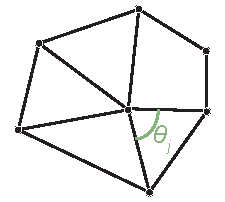
\includegraphics{images/PointIncidentAngles}
\hfill~

\noindent
We want a worklet to compute $\sum_{j} \theta$ for all such attached angles.
This measure is related (but not the same as) the curvature of the surface.
A flat surface will have a sum of $2\pi$.
Convex and concave surfaces have a value less than $2\pi$, and saddle surfaces have a value greater than $2\pi$.

To do this, we create a map cell to point worklet (Section~\ref{sec:WorkletMapCellToPoint}) that visits every point and gives the index of every incident cell.
The worklet then uses a whole cell set to inspect each incident cell to measure the attached angle and sum them together.

\vtkmlisting{Using \protect\sigtag{WholeCellSetIn} to sum the angles around each point.}{SumOfAngles.cxx}

\index{control~signature!whole cell set|)}
\index{worklet!whole cell set|)}
\index{cell~set!whole|)}
\index{whole cell set|)}

\section{Execution Objects}
\label{sec:ExecutionObjects}

\index{execution~object|(}
\index{worklet!execution~object|(}
\index{control~signature!execution~object|(}

Although passing whole arrays and cell sets into a worklet is a convenient way to provide data to a worklet that is not divided by the input or output domain, they is sometimes not the best structures to represent data.
Thus, all worklets support a another type of argument called an \keyterm{execution object}, or exec object for short, that passes the given object directly to each invocation of the worklet.
This is defined by an \sigtag{ExecObject} tag in the \controlsignature.

The execution object must be a subclass of \vtkmexec{ExecutionObjectBase}.
Also, it must be possible to copy the object from the control environment
to the execution environment and be usable in the execution environment,
and any method of the execution object used within the worklet must be
declared with \vtkmexecmodifier or \vtkmexeccontmodifier.

An execution object can refer to an array, but the array reference must be
through an array portal for the execution environment. This can be
retrieved from the \textcode{PrepareForInput} method in
\vtkmcont{ArrayHandle} as described in
Section~\ref{sec:ArrayHandle:InterfaceToExecutionEnvironment}. Other VTK-m
data objects, such as the subclasses of \vtkmcont{CellSet}, have similar
methods.

Returning to the example we have in Section~\ref{sec:WholeArrays}, we are
computing triangle quality quickly by looking up the value in a table. In
Example~\ref{ex:TriQualityWholeArray} the table is passed directly to the
worklet as a whole array. However, there is some additional code involved
to get the appropriate index into the table for a given triangle. Let us
say that we want to have the ability to compute triangle quality in many
different worklets. Rather than pass in a raw array, it would be better to
encapsulate the functionality in an object.

We can do that by creating an execution object that has the table stored
inside and methods to compute the triangle quality. The following example
uses the table built in Example~\ref{ex:TriQualityWholeArray} to create
such an object.

\vtkmlisting[ex:TriQualityExecObject]{Using \protect\sigtag{ExecObject} to access a lookup table in a worklet.}{TriangleQualityExecObject.cxx}

\index{control~signature!execution~object|)}
\index{worklet!execution~object|)}
\index{execution~object|)}

\section{Scatter}
\label{sec:WorkletScatter}

\index{scatter|(}
\index{worklet!scatter|(}

The default scheduling of a worklet provides a 1 to 1 mapping from the
input domain to the output domain. For example, a
\vtkmworklet{WorkletMapField} gets run once for every item of the input
array and produces one item for the output array. Likewise,
\vtkmworklet{WorkletMapPointToCell} gets run once for every cell in the
input topology and produces one associated item for the output field.

However, there are many operations that do not fall well into this 1 to 1
mapping procedure. The operation might need to pass over elements that
produce no value or the operation might need to produce multiple values for
a single input element.

Such non 1 to 1 mappings can be achieved by defining a \keyterm{scatter}
for a worklet. The following types of scatter are provided by VTK-m.

\begin{description}
\item[\vtkmworklet{ScatterIdentity}] Provides a basic 1 to 1 mapping from
  input to output. This is the default scatter used if none is specified.
\item[\vtkmworklet{ScatterUniform}] Provides a 1 to many mapping from input
  to output with the same number of outputs for each input. The worklet
  provides a number at runtime that defines the number of output values to
  produce per input.
\item[\vtkmworklet{ScatterCounting}] Provides a 1 to any mapping from input
  to output with different numbers of outputs for each input. The worklet
  provides an \textidentifier{ArrayHandle} that is the same size as the
  input containing the count of output values to produce for each input.
  Values can be zero, in which case that input will be skipped.
\end{description}

To define a scatter procedure, the worklet must provide two items. The
first item is a type definition named \scattertype. The \scattertype
must be set to one of the aforementioned
\textidentifier{Scatter*} classes. The second item is a \textcode{const}
method named \textcode{GetScatter} that returns an object of type
\scattertype.

\vtkmlisting{Declaration of a scatter type in a worklet.}{DeclareScatter.cxx}

When using a scatter that produces multiple outputs for a single input, the worklet is invoked multiple times with the same input values.
In such an event the worklet operator needs to distinguish these calls to produce the correct associated output.
This is done by declaring one of the \executionsignature arguments as \index{visit~index} \sigtag{VisitIndex}.
This tag will pass a \vtkm{IdComponent} to the worklet that identifies which invocation is being called.

It is also the case that the when a scatter can produce multiple outputs for some input that the index of the input element is not the same as the \sigtag{WorkIndex}.
If the index to the input element is needed, you can use the \index{input index} \sigtag{InputIndex} tag in the \executionsignature.
It is also good practice to use the \index{output index} \sigtag{OutputIndex} tag if the index to the output element is needed.

To demonstrate using scatters with worklets, we provide some contrived but
illustrative examples. The first example is a worklet that takes a pair of
input arrays and interleaves them so that the first, third, fifth, and so
on entries come from the first array and the second, fourth, sixth, and so
on entries come from the second array. We achieve this by using a
\vtkmcont{ScatterUniform} of size 2 and using the \sigtag{VisitIndex} to
determine from which array to pull a value.

\vtkmlisting{Using \textidentifier{ScatterUniform}.}{ScatterUniform.cxx}

The second example takes a collection of point coordinates and clips them
by an axis-aligned bounding box. It does this using a
\vtkmcont{ScatterCounting} with an array containing 0 for all points
outside the bounds and 1 for all points inside the bounds. As is typical
with this type of operation, we use another worklet with a default identity
scatter to build the count array.

\vtkmlisting{Using \textidentifier{ScatterCounting}.}{ScatterCounting.cxx}

\index{worklet!scatter|)}
\index{scatter|)}


\section{Error Handling}
\label{sec:ExecutionEnvironment:ErrorHandling}
\label{sec:Worklet:ErrorHandling}

\index{errors|(}

\index{errors!execution~environment|(}
\index{errors!worklet|(}
\index{worklet!error~handling|(}

It is sometimes the case during the execution of an algorithm that an error
condition can occur that causes the computation to become invalid. At such
a time, it is important to raise an error to alert the calling code of the
problem. Since VTK-m uses an exception mechanism to raise errors, we want
an error in the execution environment to throw an exception.

However, throwing exceptions in a parallel algorithm is problematic. Some
accelerator architectures, like CUDA, do not even support throwing
exceptions. Even on architectures that do support exceptions, throwing them
in a thread block can cause problems. An exception raised in one thread may
or may not be thrown in another, which increases the potential for
deadlocks, and it is unclear how uncaught exceptions progress through
thread blocks.

VTK-m handles this problem by using a flag and check mechanism. When a
worklet (or other subclass of \vtkmexec{FunctorBase}) encounters an error,
it can call its \textcode{RaiseError} method to flag the problem and record
a message for the error. Once all the threads terminate, the scheduler
checks for the error, and if one exists it throws a
\vtkmcont{ErrorExecution} exception in the control environment. Thus,
calling \textcode{RaiseError} looks like an exception was thrown from the
perspective of the control environment code that invoked it.

\vtkmlisting{Raising an error in the execution environment.}{ExecutionErrors.cxx}

\index{worklet!error~handling|)}
\index{errors!worklet|)}
\index{errors!execution~environment|)}

\index{errors!assert|(}
\index{assert|(}

It is also worth noting that the \vtkmmacro{VTKM\_ASSERT} macro described
in Section~\ref{sec:ErrorHandlingControl} also works within worklets and
other code running in the execution environment. Of course, a failed assert
will terminate execution rather than just raise an error so is best for
checking invalid conditions for debugging purposes.

\index{assert|)}
\index{errors!assert|)}

\index{errors|)}

\index{worklet!creating|)}
\index{worklet|)}


% -*- latex -*-

\chapter{Advanced Worklet Customization}
\label{chap:AdvancedWorklets}

\fix{This chapter should be split up.}

Chapter~\ref{chap:Worklets} describes the basics of creating and using
worklets. Many visualization algorithms can be implemented using VTK-m's
existing worklet types and features. However, new algorithms and designs
may require features not provided by VTK-m's current worklet set. In such
cases it is possible to directly design filters using the lower level
device adapter operations \fix{as described in section bla}. But by adding
features to the worklet mechanisms, new designs can be integrated better
with the other VTK-m features and can be repurposed in interesting ways for
other algorithms.

This chapter provides the information necessary to create new mechanisms
for worklets. It first describes the interface for getting data from the
control environment objects to the data passed to a worklet invocation and
back. It then describes how to modify these mechanisms to create new data
movement structures and new worklet types.

\section{Transferring Arguments from Control to Execution}
\label{sec:TransferringArguments}

From the \controlsignature and \executionsignature defined in worklets,
VTK-m uses template meta-programming to build the code required to manage
data from control to execution environment. This management is handled by
three classes that provide type checking, transportation, and fetching.

\fix{I've been thinking that one more feature that these classes should
  provide is the ability to return the size of the domain. That would make
  things simpler and safer for getting the input domain size and checking
  the remaining domain sizes.}

\subsection{Type Checks}
\label{sec:TypeChecks}

\index{type~check|(}

Before attempting to move data from the control to the execution
environment, the VTK-m dispatchers check the input types to ensure that
they are compatible with the associated \controlsignature concept. This is
done with the \vtkmcontarg{TypeCheck} \textcode{struct}.

The \textidentifier{TypeCheck} \textcode{struct} is templated with two
parameters. The first parameter is a tag that identifies which check to
perform. The second parameter is the type of the control argument (after any
dynamic casts). The \textidentifier{TypeCheck} class contains a static
constant Boolean named \textcode{value} that is \textcode{true} if the type
in the second parameter is compatible with the tag in the first or
\textcode{false} otherwise.

Type checks are implemented with a defined type check tag (which, by
convention, is defined in the \vtkmcontarg{} namespace and starts with
\textcode{TypeCheckTag}) and a partial specialization of the
\vtkmcontarg{TypeCheck} structure. The following type checks (identified by
their tags) are provided in VTK-m.

\begin{description}
\item[\vtkmcontarg{TypeCheckTagArray}] \index{type~check!array} True if the
  type is a \vtkmcont{ArrayHandle}. \textidentifier{TypeCheckTagArray} also
  has a template parameter that is a type list. The
  \textidentifier{ArrayHandle} must also have a value type contained in
  this type list.
\item[\vtkmcontarg{TypeCheckTagExecObject}]
  \index{type~check!execution~object} True if the type is an execution
  object. All execution objects must derive from
  \vtkmexec{ExecutionObjectBase} and must be copyable through
  \textcode{memcpy} or similar mechanism.
\end{description}

Here are some trivial examples of using
\textidentifier{TypeCheck}. Typically these checks are done internally in
the base VTK-m dispatcher code, so these examples are for demonstration
only.

\vtkmlisting{Behavior of \protect\vtkmcontarg{TypeCheck}.}{TypeCheck.cxx}

\index{type~check|)}

\subsection{Transport}
\label{sec:Transport}

\index{transport|(}

After all the argument types are checked, the base dispatcher must load the
data into the execution environment before scheduling a job to run
there. This is done with the \vtkmcontarg{Transport} \textcode{struct}.

The \textidentifier{Transport} \textcode{struct} is templated with three
parameters. The first parameter is a tag that identifies which transport to
perform. The second parameter is the type of the control parameter (after any
dynamic casts). The third parameter is a device adapter tag for the device
on which the data will be loaded.

A \textidentifier{Transport} contains a \textcode{typedef} named \textcode{ExecObjectType} that is the type used after data is moved to the execution environment.
A \textidentifier{Transport} also has a \textcode{const} parenthesis operator that takes the control-side object that is to be transported to the execution environment, the control-side object that represents the input domain, and the size of the output domain and returns an execution-side object.
This operator is called in the control environment, and the returned object must be ready to be passed to the execution environment.

Transports are implemented with a defined transport tag (which, by
convention, is defined in the \vtkmcontarg{} namespace and starts with
\textcode{TransportTag}) and a partial specialization of the
\vtkmcontarg{Transport} structure. The following transports (identified by
their tags) are provided in VTK-m.

\begin{description}
\item[\vtkmcontarg{TransportTagArrayIn}] \index{transport!input~array}
  Loads data from a \vtkmcont{ArrayHandle} onto the specified device using
  the array handle's \textcode{PrepareForInput} method. The returned
  execution object is an array portal.
\item[\vtkmcontarg{TransportTagArrayOut}] \index{transport!output~array}
  Allocates data onto the specified device for a \vtkmcont{ArrayHandle}
  using the array handle's \textcode{PrepareForOutput} method. The returned
  execution object is an array portal.
\item[\vtkmcontarg{TransportTagExecObject}]
  \index{transport!execution~object} Simply returns the given execution
  object, which should be ready to load onto the device.
\end{description}

Here are some trivial examples of using
\textidentifier{Transport}. Typically this movement is done internally in
the base VTK-m dispatcher code, so these examples are for demonstration
only.

\vtkmlisting{Behavior of \protect\vtkmcontarg{Transport}.}{Transport.cxx}

\index{transport|)}

\subsection{Fetch}
\label{sec:Fetch}

\index{fetch|(}

Before the function of a worklet is invoked, the VTK-m internals pull the
appropriate data out of the execution object and pass it to the worklet
function. A class named \vtkmexecarg{Fetch} is responsible for pulling this
data out and putting computed data in to the execution objects.

The \textidentifier{Fetch} \textcode{struct} is templated with four
parameters. The first parameter is a tag that identifies which type of
fetch to perform. The second parameter is a different tag that identifies
the aspect of the data to fetch. The third parameter is an
\textidentifier{Invocation} type that provides details about how the
worklet is being dispatched including a list of execution object parameters
passed to the invocation. The fourth parameter is a \vtkm{IdComponent} that
points to the invocation parameter that the data should be fetched from.

A \textidentifier{Fetch} contains a \textcode{typedef} named
\textcode{ValueType} that is the type of data that is passed to and from
the worklet function. A \textidentifier{Fetch} also has a pair of methods
named \textcode{Load} and \textcode{Store} that get data from and add data
to the execution object at a given domain or thread index.

\index{aspect|(}
\index{fetch!aspect|see{aspect}}

Fetches are specified with a pair of fetch and aspect tags. Fetch tags are by
convention defined in the \vtkmexecarg{} namespace and start with
\textcode{FetchTag}. Likewise, aspect tags are also defined in the
\vtkmexecarg{} namespace and start with \textcode{AspectTag}. The
\textidentifier{Fetch} \textcode{typedef} is partially specialized on these
two tags.

\index{aspect!default} The most common aspect tag is
\vtkmexecarg{AspectTagDefault}, and all fetch tags should have a
specialization of \vtkmexecarg{Fetch} with this tag. The following list of
fetch tags describes the execution objects they work with and the data they
pull for each aspect tag they support.

\fix{Don't forget to add index entries for both fetch and aspect where
  appropriate.}

\begin{description}
\item[\vtkmexecarg{FetchTagArrayDirectIn}] \index{fetch!direct input array}
  Loads data from an array portal. This fetch only supports the
  \textidentifier{AspectTagDefault} aspect. The \textcode{Load} gets data
  directly from the domain (thread) index. The \textcode{Store} does
  nothing.
\item[\vtkmexecarg{FetchTagArrayDirectOut}] \index{fetch!direct output array}
  Stores data to an array portal. This fetch only supports the
  \textidentifier{AspectTagDefault} aspect. The \textcode{Store} sets data
  directly to the domain (thread) index. The \textcode{Load} does nothing.
\item[\vtkmexecarg{FetchTagExecObject}] \index{fetch!execution object}
  Simply returns an execution object. This fetch only supports the
  \textidentifier{AspectTagDefault} aspect. The \textcode{Load} returns the
  executive object in the associated parameter. The \textcode{Store} does
  nothing.
\end{description}

In addition to the aforementioned aspect tags that are explicitly paired
with fetch tags, VTK-m also provides some aspect tags that either modify
the behavior of a general fetch or simply ignore the type of fetch.

\begin{description}
\item[\vtkmexecarg{AspectTagWorkIndex}] \index{aspect!work index} Simply
  returns the domain (or thread) index ignoring any associated data. This
  aspect is used to implement the \sigtag{WorkIndex} execution signature
  tag.
\end{description}

\index{aspect|)}
\index{fetch|)}


\section{Function Interface Objects}
\label{sec:FunctionInterfaceObjects}

\index{function~interface|(}

For flexibility's sake a worklet is free to declare a \controlsignature
with whatever number of arguments are sensible for its operation. The
\textcode{Invoke} method of the dispatcher is expected to support arguments
that match these arguments, and part of the dispatching operation may
require these arguments to be augmented before the worklet is
scheduled. This leaves dispatchers with the tricky task of managing some
collection of arguments of unknown size and unknown types.

\fix{\textidentifier{FunctionInterface} is in the \vtkminternal{}
  interface. I still can't decide if it should be moved to the \vtkm{}
  interface.}

To simplify this management, VTK-m has the \vtkminternal{FunctionInterface}
class. \textidentifier{FunctionInterface} is a templated class that manages
a generic set of arguments and return value from a function. An instance of
\textidentifier{FunctionInterface} holds an instance of each argument. You
can apply the arguments in a \textidentifier{FunctionInterface} object to a
functor of a compatible prototype, and the resulting value of the function
call is saved in the \textidentifier{FunctionInterface}.

\subsection{Declaring and Creating}

\vtkminternal{FunctionInterface} is a templated class with a single
parameter. The parameter is the \index{function~signature}
\index{signature} \keyterm{signature} of the function. A signature is a
function type. The syntax in C++ is the return type followed by the
argument types encased in parentheses.

\vtkmlisting{Declaring \protect\vtkminternal{FunctionInterface}.}{DefineFunctionInterface.cxx}

The \vtkminternal{make\_FunctionInterface} function provies an easy way to
create a \textidentifier{FunctionInterface} and initialize the state of all
the parameters. \textidentifier{make\_FunctionInterface} takes a variable
number of arguments, one for each parameter. Since the return type is not
specified as an argument, you must always specify it as a template
parameter.

\vtkmlisting{Using \protect\vtkminternal{make\_FunctionInterface}.}{UseMakeFunctionInterface.cxx}

\subsection{Parameters}

One created, \textidentifier{FunctionInterface} contains methods to query
and manage the parameters and objects associated with them. The number of
parameters can be retrieved either with the constant field \index{arity}
\textcode{ARITY} or with the \textcode{GetArity} method.

\vtkmlisting{Getting the arity of a \textidentifier{FunctionInterface}.}{FunctionInterfaceArity.cxx}

To get a particular parameter, \textidentifier{FunctionInterface} has the
templated method \textcode{GetParameter}. The template parameter is the
index of the parameter. Note that the parameters in
\textidentifier{FunctionInterface} start at index 1. Although this is
uncommon in C++, it is customary to number function arguments starting at
1.

There are two ways to specify the index for \textcode{GetParameter}. The
first is to directly specify the template parameter (e.g.
\textcode{GetParameter<1>()}). However, note that in a templated function
or method where the type is not fully resolved the compiler will not
register \textcode{GetParameter} as a templated method and will fail to
parse the template argument without a \textcode{template} keyword. The
second way to specify the index is to provide a \vtkminternal{IndexTag}
object as an argument to \textcode{GetParameter}. Although this syntax is
more verbose, it works the same whether the
\textidentifier{FunctionInterface} is fully resolved or not. The following
example shows both methods in action.

\vtkmlisting{Using \textidentifier{FunctionInterface}\textcode{::GetParameter().}}{FunctionInterfaceGetParameter.cxx}

Likewise, there is a \textcode{SetParmeter} method for changing parameters.
The same rules for indexing and template specification apply.

\vtkmlisting{Using \textidentifier{FunctionInterface}\textcode{::SetParameter().}}{FunctionInterfaceSetParameter.cxx}

\subsection{Invoking}

\index{function~interface!invoke|(}

\textidentifier{FunctionInterface} can invoke a functor of a matching
signature using the parameters stored within. If the functor returns a
value, that return value will be stored in the
\textidentifier{FunctionInterface} object for later retrieval. There are
several versions of the invoke method. There are always seperate versions
of invoke methods for the control and execution environments so that
functors for either environment can be executed. The basic version of
invoke passes the parameters directly to the function and directly stores
the result.

\vtkmlisting{Invoking a \textidentifier{FunctionInterface}.}{FunctionInterfaceBasicInvoke.cxx}

Another form of the invoke methods takes a second transform functor that is
applied to each argument before passed to the main function. If the main
function returns a value, the transform is applied to that as well before
being stored back in the \textidentifier{FunctionInterface}.

\vtkmlisting{Invoking a \textidentifier{FunctionInterface} with a transform.}{FunctionInterfaceTransformInvoke.cxx}

\index{function~interface!invoke|)}

As demonstrated in the previous examples,
\textidentifier{FunctionInterface} has a method named
\textcode{GetReturnValue} that returns the value from the last invoke. Care
should be taken to only use \textcode{GetReturnValue} when the function
specification has a return value. If the function signature has a
\textcode{void} return type, using \textcode{GetReturnValue} will cause a
compile error.

\textidentifier{FunctionInterface} has an alternate method named
\textcode{GetReturnValueSafe} that returns the value wrapped in a templated
structure named \vtkminternal{FunctionInterfaceReturnContainer}. This
structure always has a static constant Boolean named \textcode{VALID} that
is \textcode{false} if there is no return type and \textcode{true}
otherwise. If the container is valid, it also has an entry named
\textcode{Value} containing the result.

\vtkmlisting{Getting return value from \textidentifier{FunctionInterface} safely.}{FunctionInterfaceReturnContainer.cxx}

\subsection{Modifying Parameters}

In addition to storing and querying parameters and invoking functions,
\textidentifier{FunctionInterface} also contains multiple ways to modify
the parameters to augment the function calls. This can be used in the same
use case as a chain of function calls that generally pass their parameters
but also augment the data along the way.

\index{function~interface!append parameter|(}

The \textcode{Append} method returns a new
\textidentifier{FunctionInterface} object with the same parameters plus a
new parameter (the argument to \textcode{Append}) to the end of the
parameters. There is also a matching \textcode{AppendType} templated
structure that can return the type of an augmented
\textidentifier{FunctionInterface} with a new type appended.

\vtkmlisting{Appending parameters to a \textidentifier{FunctionInterface}.}{FunctionInterfaceAppend.cxx}

\index{function~interface!append parameter|)}

\index{function~interface!replace parameter|(}

\textcode{Replace} is a similar method that returns a new
\textidentifier{FunctionInterface} object with the same paraemters except
with a specified parameter replaced with a new parameter (the argument to
\textcode{Replace}). There is also a matching \textcode{ReplaceType}
templated structure that can return the type of an augmented
\textidentifier{FunctionInterface} with one of the parameters replaced.

\vtkmlisting{Replacing parameters in a \textidentifier{FunctionInterface}.}{FunctionInterfaceReplace.cxx}

\index{function~interface!replace parameter|)}

It is sometimes desirable to make multiple modifications at a time. This
can be achieved by chaining modifications by calling \textcode{Append} or
\textcode{Replace} on the result of a previous call.

\vtkmlisting{Chaining \textcode{Replace} and \textcode{Append} with a \textidentifier{FunctionInterface}.}{FunctionInterfaceAppendAndReplace.cxx}

\subsection{Transformations}

Rather than replace a single item in a \textidentifier{FunctionInterface},
it is sometimes desirable to change them all in a similar
way. \textidentifier{FunctionInterface} supports two basic transform
operations on its parameters: a static transform and a dynamic
transform. The static transform determines its types at compile-time
whereas the dynamic transform happens at run-time.

\index{function~interface!static transform|(}

The static transform methods (named \textcode{StaticTransformCont} and
\textcode{StaticTransformExec}) operate by accepting a functor that defines
a function with two arguments. The first argument is the
\textidentifier{FunctionInterface} parameter to transform. The second
argument is an instance of the \vtkminternal{IndexTag} templated class that
statically identifies the parameter index being transformed. An
\textidentifier{IndexTag} object has no state, but the class contains a
static integer named \textidentifier{INDEX}. The function returns the
transformed argument.

The functor must also contain a templated class named \textcode{ReturnType}
with an internal type named \textcode{type} that defines the return type of
the transform for a given parameter type. \textcode{ReturnType} must have
two template parameters. The first template parameter is the type of the
\textidentifier{FunctionInterface} parameter to transform. It is the same
type as passed to the operator. The second template parameter is a
\vtkm{IdComponent} specifying the index.

The transformation is only applied to the parameters of the function. The
return argument is unaffected.

The return type can be determined with the \textcode{StaticTransformType}
template in the \textidentifier{FunctionInterface}
class. \textcode{StaticTransformType} has a single parameter that is the
transform functor and contains a type named \textcode{type} that is the
transformed \textidentifier{FunctionInterface}.

In the following example, a static transform is used to convert a
\textidentifier{FunctionInterface} to a new object that has the pointers to
the parameters rather than the values themselves. The parameter index is
always ignored as all parameters are uniformly transformed.

\vtkmlisting{Using a static transform of function interface class.}{FunctionInterfaceStaticTransform.cxx}

\index{function~interface!static transform|)}

\index{function~interface!dynamic transform|(}

There are cases where one set of parameters must be transformed to another
set, but the types of the new set are not known until run-time. That is,
the transformed type depends on the contents of the data. The
\textcode{DynamicTransformCont} method achieves this using a templated
callback that gets called with the correct type at run-time.

The dynamic transform works with two functors provided by the user code (as
opposed to the one functor in static transform). These functors are called
the transform functor and the finish functor. The transform functor accepts
three arguments. The first argument is a parameter to transform. The second
argument is a continue function. Rather than return the transformed value,
the transform functor calls the continue function, passing the transformed
value as an argument. The third argument is a \vtkminternal{IndexTag} for
the index of the argument being transformed.

Unlike its static counterpart, the dynamic transform method does not return
the transformed \textidentifier{FunctionInterface}. Instead, it passes the
transformed \textidentifier{FunctionInterface} to the finish functor passed
into \textcode{DynamicTransformCont}.

In the following contrived but illustrative example, a dynamic transform is
used to convert strings containing numbers into number arguments. Strings
that do not have numbers and all other arguments are passed through. Note
that because the types for strings are not determined till run-time, this
transform cannot be determined at compile time with meta-template
programming. The index argument is ignored because all arguments are
transformed the same way.


\vtkmlisting{Using a dynamic transform of a function interface.}{FunctionInterfaceDynamicTransform.cxx}

One common use for the \textidentifier{FunctionInterface} dynamic transform
is to convert parameters of virtual polymorphic type like
\vtkmcont{DynamicArrayHandle} and \vtkmcont{DynamicPointCoordinates}. This
use case is handled with a functor named
\vtkmcontinternal{DynamicTransform}. When used as the dynamic transform
functor, it will convert all of these dynamic types to their static
counterparts.

\vtkmlisting{Using \textidentifier{DynamicTransform} to cast dynamic arrays in a function interface.}{DynamicTransform.cxx}

\index{function~interface!dynamic transform|)}

\subsection{For Each}
\label{sec:FunctionInterface:ForEach}

\index{function~interface!for~each|(}

The invoke methods (principally) make a single function call passing all of
the parameters to this function. The transform methods call a function on
each parameter to convert it to some other data type. It is also sometimes
helpful to be able to call a unary function on each parameter that is not
expected to return a value. Typically the use case is for the function to
have some sort of side effect. For example, the function might print out
some value (such as in the following example) or perform some check on the
data and throw an exception on failure.

This feature is implemented in the for each methods of
\textidentifier{FunctionInterface}.  As with all the
\textidentifier{FunctionInterface} methods that take functors, there are
separate implementations for the control environment and the execution
environment. There are also separate implementations taking
\textcode{const} and non-\textcode{const} references to functors to
simplify making functors with side effects.

\vtkmlisting{Using the \textcode{ForEach} feature of \textidentifier{FunctionInterface}.}{FunctionInterfaceForEach.cxx}

\index{function~interface!for~each|)}

\index{function~interface|)}


\section{Invocation Objects}
\label{sec:InvocationObjects}


\section{Creating New \protect\controlsignature Tags}
\label{sec:NewControlSignatureTags}


\section{Creating New \protect\executionsignature Tags}
\label{sec:NewExecutionSignatureTags}


\section{Creating New Worklet Types}
\label{sec:NewWorkletTypes}

\subsection{New Worklet Superclasses}
\label{sec:NewWorkletSuperclasses}

\subsection{Dispatch Workflow}
\label{sec:DispatchWorkflow}

\subsection{New Dispatch Classes}
\label{sec:NewDispatchClasses}


\chapter{OpenGL Interoperability}
\label{chap:OpenGLInteroperability}

% -*- latex -*-

\chapter{Coding Conventions}
\label{chap:CodingConventions}

Several developers contribute to VTK-m and we welcome others who are
interested to also contribute to the project. To ensure readability and
consistency in the code, we have adopted the following coding
conventions. Many of these conventions are adapted from the coding
conventions of the VTK project. This is because many of the developers are
familiar with VTK coding and because we expect VTK-m to have continual
interaction with VTK.

\begin{itemize}
\item All code contributed to VTK-m must be compatible with VTK-m's BSD
  license.
\item Copyright notices should appear at the top of all source,
  configuration, and text files. The statement should have the following
  form (with the year replaced with the year the file was created):
\small\begin{verbatim}
//============================================================================
//  Copyright (c) Kitware, Inc.
//  All rights reserved.
//  See LICENSE.txt for details.
//  This software is distributed WITHOUT ANY WARRANTY; without even
//  the implied warranty of MERCHANTABILITY or FITNESS FOR A PARTICULAR
//  PURPOSE.  See the above copyright notice for more information.
//
//  Copyright 2014 Sandia Corporation.
//  Copyright 2014 UT-Battelle, LLC.
//  Copyright 2014. Los Alamos National Security
//
//  Under the terms of Contract DE-AC04-94AL85000 with Sandia Corporation,
//  the U.S. Government retains certain rights in this software.
//
//  Under the terms of Contract DE-AC52-06NA25396 with Los Alamos National
//  Laboratory (LANL), the U.S. Government retains certain rights in
//  this software.
//============================================================================
\end{verbatim}
  The \textfilename{CopyrightStatement} test checks all files for a similar
  statement. The test will print out a suggested text that can be copied
  and pasted to any file that has a missing copyright statement (with
  appropriate replacement of comment prefix). Exceptions to this copyright
  statement (for example, third-party files with different but compatible
  statements) can be added to \textfilename{LICENSE.txt}.
\item All include files should use include guards. starting right after the
  copyright statement. The naming convention of the include guard macro is
  that it should start with \textcode{vtk\_m} be followed with the path
  name, starting from the top-level source code directory under
  \textfilename{vtkm}, with non alphanumeric characters, such as
  \textcode{/} and \textcode{.} replaced with underscores. The
  \textcode{\#endif} part of the guard at the bottom of the file should
  include the guard name in a comment. For example, the
  \vtkmheader{vtkm/cont}{ArrayHandle.h} header contains the guard
\begin{verbatim}
#ifndef vtk_m_cont_ArrayHandle_h
#define vtk_m_cont_ArrayHandle_h
\end{verbatim}
  at the top and
\begin{verbatim}
#endif //vtk_m_cont_ArrayHandle_h
\end{verbatim}
\item VTK-m has several nested namespaces. The declaration of each
  namespace should be on its own line, and the code inside the namespace
  bracket should not be indented. The closing brace at the bottom of the
  namespace should be documented with a comment identifying the
  namespace. Namespaces can be grouped as desired. The following is a valid
  use of namespaces.
\begin{verbatim}
namespace vtkm {
namespace cont {

namespace detail {

class InternalClass;

} // namespace detail

class ExposedClass;

}
} // namespace vtkm::cont
\end{verbatim}
\item Multiple inheritance is not allowed in VTK-m classes.
\item Any functional public class should be in its own header file with the
  same name as the class. The file should be in a directory that
  corresponds to the namespace the class is in. There are several
  exceptions to this rule.
  \begin{itemize}
  \item Templated classes and template specialization often require the
    implementation of the class to be broken into pieces. Sometimes a
    specialization is placed in a header with a different name.
  \item Many VTK-m toolkit features are not encapsulated in
    classes. Functions may be collected by purpose or co-located with
    associated class.
  \item Although tags are technically classes, they behave as an
    enumeration for the compiler. Multiple tags that make up this
    enumeration are collected together.
  \item Some classes, such as \vtkm{Vec} are meant to behave as basic
    types. These are sometimes collected together as if they were related
    \textcode{typedef}s. The \vtkmheader{vtkm}{Types.h} header is a good
    example of this.
  \end{itemize}
\item The indentation follows the Allman style. The curly brace (scope
  delimiter) for a block is placed on the line following the prototype or
  control statement and is indented with the outer scope (i.e. the curly
  brace does not line up with the code in the block). This differs from VTK
  style, but was agreed on by the developers as the more common
  style. Indentations are two spaces.
\item Conditional clauses (including loop conditionals such as
  \textcode{for} and \textcode{while}) must be in braces below the
  conditional. That is, instead of
\begin{verbatim}
if (test) { clause; }
\end{verbatim}
  use
\begin{verbatim}
if (test)
{
  clause;
}
\end{verbatim}
  The rational for this requirement is to make it obvious whether the
  clause is executed when stepping through the code with the debugger. The
  one exception to this rule is when the clause contains a control-flow
  statement with obvious side effects such as \textcode{return} or
  \textcode{break}. However, even if the clause contains a single statement
  and is on the same line, the clause should be surrounded by braces.
\item Use two space indentation.
\item Tabs are not allowed. Only use spaces for indentation. No one can
  agree on what the size of a tab stop is, so it is better to not use them
  at all.
\item There should be no trailing whitespace in any line.
\item Use only alphanumeric characters in names. Use capitalization to
  demarcate words within a name (camel case). The exception is preprocessor
  macros and constant numbers that are, by convention, represented in all
  caps and a single underscore to demarcate words.
\item Namespace names are in all lowercase. They should be a single word
  that designates its meaning.
\item All class, method, member variable, and functions should start with a
  capital letter. Local variables should start in lower case and then use
  camel case. Exceptions can be made when such naming would conflict with
  previously established conventions in other library. (For example,
  \textcode{make\_ArrayHandle} corresponds to \textcode{make\_pair} in the
  standard template library.)
\item All class, function, and member names that have multiple words in
  their descriptions should be listed from general to specific. For
  example, if a class is a k-d tree that is used to locate points, the
  preferred name would be \textcode{LocatorPointKDTree}. This naming
  convention makes it easier to find both known and unknown classes in
  alphabetic lists.
\item Always spell out words in names; do not use abbreviations except in
  cases where the shortened form is widely understood and a name in its own
  right (e.g. OpenMP).
\item Always use descriptive names in all identifiers, including local
  variable names. Particularly avoid meaningless names of a few characters
  (e.g. \textcode{x}, \textcode{foo}, or \textcode{tmp}) or numbered names
  with no meaning to the number or order (e.g. \textcode{value1},
  \textcode{value2},\ldots). Also avoid the meaningless for loop variable
  names \textcode{i}, \textcode{j}, \textcode{k}, etc. Instead, use a name
  that identifies what type of index is being referenced such as
  \textcode{pointIndex}, \textcode{vertexIndex}, \textcode{componentIndex},
  etc.
\item Classes are documented with Doxygen-style comments before classes,
  methods, and functions.
\item Exposed classes should not have public instance variables outside of
  exceptional situations. Access is given by convention through methods
  with names starting with \textcode{Set} and \textcode{Get} or through
  overloaded operators.
\item References to classes and functions should be fully qualified with
  the namespace. This makes it easier to establish classes and functions
  from different packages and to find source and documentation for the
  referenced class. As an exception, if one class references an internal or
  detail class clearly associated with it, the reference can be shortened
  to \textcode{internal::} or \textcode{detail::}.
\item use \textcode{this->} inside of methods when accessing class methods
  and instance variables to distinguish between local variables and
  instance variables.
\item Include statements should generally be in alphabetical order. They
  can be grouped by package and type.
\item Namespaces should not be brought into global scope or the scope of
  any VTK-m package namespace with the ``using'' keyword. It should also be
  avoided in class, method, and function scopes (fully qualified namespace
  references are preferred).
\item All code must be valid by the C++11 specification.
\item Limit all lines to 80 characters whenever possible.
\item New code must include regression tests that will run on the
  dashboards. Generally a new class will have an associated ``UnitTest''
  that will test the operation of the test directly. There may be other
  tests necessary that exercise the operation with different components or
  on different architectures.
\item All code must compile and run without error or warning messages on
  the nightly dashboards, which should include Windows, Mac, and Linux.
\item Use \vtkm{Id} in lieu of \textcode{int} or \textcode{long} for data
  structure indices and \vtkm{IdComponent} for component indices of
  \vtkm{Vec} and related classes (like \vtkm{VecVariable} and
  \vtkm{Matrix}).
\item Whenever possible, use templates to resolve data types like
  \textcode{float}, \textcode{double}, or vectors to make code as flexible
  as possible. If a specific data type is required, prefer the
  VTK-m--provided types like \vtkm{Float32} and \vtkm{Float64} over the
  standard C types like \textcode{float} or
  \textcode{double}. \vtkm{FloatDefault} can be used in cases where there
  is no reasonable way to specify data precision (for example, when
  generating coordinates for uniform grids), but should be use sparingly.
\item All functions and methods defined within \VTKm should be
  declared with \vtkmcontmodifier, \vtkmexecmodifier, or \vtkmexeccontmodifier.
\end{itemize}

We should note that although these conventions impose a strict statute on
VTK-m coding, these rules (other than those involving licensing and
copyright) are not meant to be dogmatic. Examples can be found in the
existing code that break these conventions, particularly when the
conventions stand in the way of readability (which is the point in having
them in the first place). For example, it is often the case that it is more
readable for a complicated \textcode{typedef} to stretch a few characters
past 80 even if it pushes past the end of a display.



\begin{flushleft}
  \clearpage
  \lhead[]{}
  \rhead[]{}
  \phantomsection
  \addcontentsline{toc}{chapter}{Index}
  \printindex
\end{flushleft}

% -*- latex -*-

\begin{SANDdistribution}[NM]
  % External Addresses
  %% \SANDdistExternal{1}{Lucy Nowell\\ U.S. Department of Energy\\ SC-21\\ 19901 Germantown Road\\ Germantown, MD 20874-1290}
  %% \SANDdistExternal{1}{Teresa Beachley\\ U.S. Department of Energy\\ SC-21\\ 19901 Germantown Road\\ Germantown, MD 20874-1290}
  %% \SANDdistExternal{1}{Berk Geveci\\ Kitware, Inc.\\ 28 Corporate Drive\\ Clifton Park, NY 12065}
  %% \SANDdistExternal{1}{Robert Maynard\\ Kitware, Inc.\\ 28 Corporate Drive\\ Clifton Park, NY 12065}
  %% \SANDdistExternal{1}{Kwan-Liu Ma\\ Department of Computer Science\\ 2063 Kemper Hall\\ University of California-Davis\\ One Shields Avenue\\ Davis, CA 95616-8562}

  \bigskip

  % Internal Addresses
  \SANDdistInternal{1}{1326}{Kenneth Moreland}{1461}
  \SANDdistInternal{1}{1327}{Ron Oldfield}{01461}
\end{SANDdistribution}


\end{document}
